\newpage\setcounter{dang}{0}
\section{TÍCH MỘT SỐ VỚI MỘT VECTƠ}
\subsection{Tóm tắt lý thuyết}
\begin{tomtat}
\subsubsection{Khái niệm}
\begin{itemize}
    \item Tích của một véc tơ $\vec{a} \neq \vec{0}$ với số thực $k>0$ là một vectơ, kí hiệu là $k\vec{a}$, cùng hướng với vectơ  $\vec{a}$ và có độ dài bằng $k |\vec{a}|$.
    \item  Tích của một véc tơ  $\vec{a} \neq \vec{0}$ với số thực $k<0$ là một véc tơ , kí hiệu là $k\vec{a}$, ngược hướng với véc tơ  $\vec{a}$ và có độ dài bằng $(-k) |\vec{a}|$.
\end{itemize}
\begin{note}
	Ta quy ước $k\vec{a}=\vec{0}$ nếu $\vec{a}=\vec{0}$ hoặc $k=0$.
\end{note}
\begin{nx}
	\textbf{}
\begin{itemize}
	\item 	véc tơ  $k\vec{a}$ có độ dài bằng $|k||\vec{a}|$ và cùng hướng với $\vec{a}$ nếu $k\ge 0 $, ngược hướng với $\vec{a}$ nếu $\vec{a}\ne \vec{0}$ và $k<0$.
	\item Hai véc tơ   $\vec{a}$ và $\vec{b} (\vec{b}\ne \vec{0})$ cùng phương khi và chỉ khi tồn tại số $k$ để $\vec{a}=k\vec{b}$.
	\item Để chứng minh ba điểm thẳng hàng ta cần chỉ ra hai véc tơ  tạo bởi các cặp điểm trong ba điểm đó cùng phương.
\end{itemize}
\end{nx}
\subsubsection{Tính chất }
\begin{tc}
	 Với hai véc tơ  $\vec{a}, \vec{b}$ và hai số thực $k, t$, ta luôn có
	 \begin{itemize}
	 	\item $k\left(t\vec{a}\right)=(kt)\vec{a}$;
	 	\item $(k+t)\vec{a}=k\vec{a}+t\vec{a}$;
	 	\item $k\left(\vec{a}+\vec{b}\right)=k\vec{a}+k\vec{b} ; k(\vec{a}-\vec{b})=k\vec{a}-k\vec{b}$;
	 	\item $1\vec{a}=\vec{a}; (-1)\vec{a}=-\vec{a}$.

	 \end{itemize}
\end{tc}
\begin{vd}%[0H1B3-2]
	Cho tam giác $ABC$. Gọi $M$ là điểm trên cạnh $BC$ sao cho $MB=2MC$. Chứng minh rằng $\vec {AM}=\dfrac{1}{3}\vec {AB}  +  \dfrac{2}{3}\vec {AC}$.
	\loigiai{
		\immini{
			Ta có
			\allowdisplaybreaks
			\begin{align*}
				\vec {AM} & =  \vec {AB}  +  \vec {BM} \\
				&=  \vec {AB}  +  \dfrac{2}{3}\vec {BC}\\&=  \vec {AB}  +  \dfrac{2}{3}\left(\vec {AC}  -  \vec {AB}\right) \\
				&=  \dfrac{1}{3}\vec {AB}  +  \dfrac{2}{3}\vec {AC}.
			\end{align*}
		}
		{
			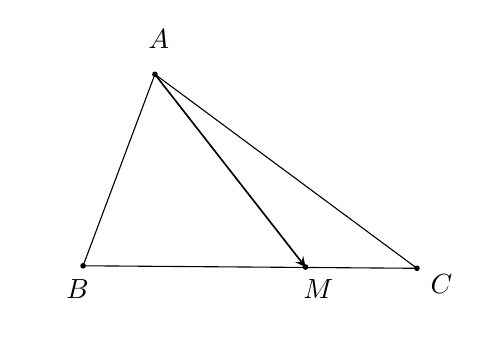
\begin{tikzpicture}[line cap=round,line join=round,>=stealth,x=1.0cm,y=1.0cm,scale=0.8]
				\clip(-0.14,0.12) rectangle (6.66,4.7);
				\draw (1.88,3.96)-- (0.74,0.92);
				\draw (0.74,0.92)-- (6.04,0.88);
				\draw (6.04,0.88)-- (1.88,3.96);
				\draw [->,line width=0.6pt] (1.88,3.96) -- (4.27,0.9);
				\draw (1.62,4.82) node[anchor=north west] {$A$};
				\draw (6.1,0.94) node[anchor=north west] {$C$};
				\draw (4.08,0.86) node[anchor=north west] {$M$};
				\draw (0.32,0.86) node[anchor=north west] {$B$};
				\begin{scriptsize}
					\draw [fill=black] (1.88,3.96) circle (1pt);
					\draw [fill=black] (0.74,0.92) circle (1pt);
					\draw [fill=black] (6.04,0.88) circle (1pt);
					\draw [fill=black] (4.27,0.9) circle (1pt);
				\end{scriptsize}
			\end{tikzpicture}
		}
	}
\end{vd}
\begin{nx}
		\textbf{}
\begin{itemize}
	\item 	Điểm $I$ là trung điểm của đoạn thẳng $AB$ khi và chỉ khi $\vec{IA}+\vec{IB}=\vec{0}$.
	\item Điểm $G$ là trọng tâm của tam giác $ABC$ khi và chỉ khi $\vec{GA}+\vec{GB}+\vec{GC}=\vec{0}$.
\end{itemize}
\end{nx}

\begin{note}
	 Cho hai véc tơ  không cùng phương $\vec{a}, \vec{b}$. Khi đó, mọi véc tơ  $\vec{u}$ đều biểu thị (phân tích) được một cách duy nhất theo hai véc tơ  $\vec{a}, \vec{b}$, nghĩa là có duy nhất cặp số $(x;y)$ sao cho $\vec{u}=x\vec{a}+y\vec{b}$.
 \end{note}
\begin{vd}%[0H1K3-3]
	Cho hình bình hành $ABCD$. Tìm $K$ thoả mãn
	$3\vec{KA}+\vec{KB}+\vec{KC}=\vec{0}$.
	\loigiai{
		\immini{
			Ta có\\
			\allowdisplaybreaks
			\begin{eqnarray*}
			&&	3\vec{KA}+\vec{KB}+\vec{KC}=\vec{0} \\
			&\Leftrightarrow& 3\vec{KC}+3\vec{CA}+\vec{KC}+\vec{CB}+\vec{KC}=\vec{0}\\
			&\Leftrightarrow& 5\vec{KC}+\vec{CA}+\vec{CB}=\vec{0}\\
			&\Leftrightarrow& 5\vec{KC}+2\vec{CN}=\vec{0} (\text{Với $N$ là trung điểm của $AB$ })\\
			&\Leftrightarrow& \vec{CK}=\dfrac{2}{5}\vec{CN}.
			\end{eqnarray*}
}
		{\begin{tikzpicture}[line cap=round,line join=round]
				\coordinate[label=below:$A$] (A)at(-2,0);
				\coordinate[label=below:$B$] (B)at(1,0);
				\coordinate[label=above:$D$] (D)at(-0.3,2);
				\coordinate[label=below:$N$] (N) at ($(A)!0.5!(B)$);
				\coordinate[label=above:$C$,shift={(0:3)}] (C) at (D);
				\coordinate[label=below:$K$] (K) at ($(N)!0.6!(C)$);
				\draw (A)--(B)--(C)--(D)--cycle (N)--(C);
 				 \foreach \x in {A,B,C,D,N,K}
 				\draw[fill=black] (\x) circle (1pt);


		\end{tikzpicture} }
			\noindent	Vậy $K$ nằm trên đoạn $CN$ và cách $C$ một đoạn là $\dfrac{2}{5}CN$ với $N$ là trung điểm $AB$.}
\end{vd}
\end{tomtat}

\subsection{Các ví dụ}

\setcounter{vd}{0}
\begin{vd}%[0H1Y3-1]
	Cho đoạn thẳng $AB$ và $M$ là một điểm nằm trên đoạn $AB$ sao cho $AM=\dfrac{1}{5}AB$. Tìm $k$ trong các đẳng thức sau
	\begin{multicols}{3}
		\begin{enumerate}[a)]
			\item $\overrightarrow{AM}=k\overrightarrow{AB}$.
			\item $\overrightarrow{MA}=k\overrightarrow{MB}$.
			\item $\overrightarrow{MA}=k\overrightarrow{AB}$.
		\end{enumerate}
	\end{multicols}
	\loigiai{
		\begin{center}
			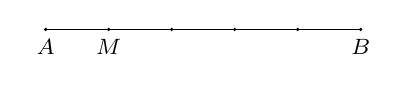
\begin{tikzpicture}[scale=0.8,>=stealth, font=\footnotesize, line join=round, line cap=round]
				\path
					(0,0) coordinate (A) (5,0) coordinate (B)
					(1,0) coordinate (M) (4,0) coordinate (F)
					(3,0) coordinate (P) (2,0) coordinate (T)
				;
				\draw (A)--(B);
				\foreach \a in {A,B,M,F,P,T} \fill[black] (\a)circle(.8pt);
				\foreach \a in {A,B,M} \draw (\a)node[below]{$\a$};
			\end{tikzpicture}
		\end{center}
		\begin{enumerate} [a)]
			\item Thấy $\overrightarrow{AM}$ và $\overrightarrow{AB}$ cùng hướng nên $k>0$. \\
			Ta có $|k|=\dfrac{|\overrightarrow{AM}|}{|\overrightarrow{AB}|}=\dfrac{AM}{AB}=\dfrac{1}{5}$. Suy ra $k=\dfrac{1}{5}$.
			\item Thấy $\overrightarrow{MA}$ và $\overrightarrow{MB}$ ngược hướng nên $k<0$. \\
			Ta có $|k|=\dfrac{|\overrightarrow{MA}|}{|\overrightarrow{MB}|}=\dfrac{AM}{MB}=\dfrac{1}{4}$. Suy ra $k=-\dfrac{1}{4}$.
			\item Thấy $\overrightarrow{MA}$ và $\overrightarrow{AB}$ ngược hướng nên $k<0$. \\
			Ta có $|k|=\dfrac{|\overrightarrow{MA}|}{|\overrightarrow{AB}|}=\dfrac{AM}{AB}=\dfrac{1}{5}$. Suy ra $k=-\dfrac{1}{5}$.
	\end{enumerate}}
\end{vd}

\begin{vd}%[0H1B3-3]
	Cho hai điểm phân biệt $A,B$. Xác định điểm $M$ biết $2\overrightarrow{MA}-3\overrightarrow{MB}=\overrightarrow{0}$.
	\loigiai{
		Ta có
		$2\overrightarrow{MA}-3\overrightarrow{MB}=\overrightarrow{0}\Leftrightarrow 2\overrightarrow{MA}-3(\overrightarrow{MA}+\overrightarrow{AB})=\overrightarrow{0}\Leftrightarrow-\overrightarrow{MA}-3\overrightarrow{AB}=\overrightarrow{0}\Leftrightarrow\overrightarrow{AM}=3\overrightarrow{AB}$. \\
		$ \Rightarrow\overrightarrow{AM},\overrightarrow{AB} $ cùng hướng và $AM=3AB$.
		\begin{center}
			\begin{tikzpicture}[scale=0.8,>=stealth, font=\footnotesize, line join=round, line cap=round]
				\tkzDefPoints{0/0/A,2/0/B,6/0/M,4/0/H}
				\tkzDrawPoints[fill=black,size=5](A,B,M,H)
				\tkzDrawSegments(A,M)
				\tkzLabelPoints[below](A,B,M)
			\end{tikzpicture}
		\end{center}
	}
\end{vd}


\begin{vd}%[0H1K3-5]
	Cho tam giác $ABC$ có trung tuyến $AM$. Gọi $I$ là trung điểm $AM$ và $K$ là  điểm thuộc $AC$ sao $AK=\dfrac{1}{3}AC$. Chứng minh ba điểm $B, I, K$ thẳng hàng.
	\loigiai{
		\immini
		{
			Ta có $2\overrightarrow{BI}=\overrightarrow{BA}+\overrightarrow{BM}=\overrightarrow{BA}+\dfrac{1}{2}\overrightarrow{BC}$ \\
			$\Rightarrow 4\overrightarrow{BI}=2\overrightarrow{BA}+\overrightarrow{BC}.\quad(1)$\\
			Ta có
			\allowdisplaybreaks
			\begin{eqnarray*}
				\overrightarrow{BK}&=&\overrightarrow{BA}+\overrightarrow{AK} \\
				&=&\overrightarrow{BA}+\dfrac{1}{3}\overrightarrow{AC} \\ &=&\overrightarrow{BA}+\dfrac{1}{3}(\overrightarrow{BC}-\overrightarrow{BA}) \\
				&=&\dfrac{2}{3}\overrightarrow{BA}+\dfrac{1}{3}\overrightarrow{BC}.
			\end{eqnarray*}
			Suy ra $3\overrightarrow{BK}=2\overrightarrow{BA}+\overrightarrow{BC}.\quad(2) $\\
		}
		{
			\begin{tikzpicture}[font=\scriptsize,scale=0.7]
				\path
				(0,0) coordinate (B)
				(1,3)  coordinate (A)
				(5,0) coordinate (C);
				\coordinate (M) at ($(B)!.5!(C)$);
				\coordinate (I) at ($(A)!.5!(M)$);
				\coordinate (K) at (intersection of B--I and A--C);

				\draw (A)--(B)--(C)--cycle	(B)--(K) (A)--(M);
				\foreach \x/\g in {A/90, B/250,C/270,M/270,I/0,K/0}
				\fill[black](\x) circle (1.5pt) ($(\x)+(\g:4mm)$)node{\x};
				\draw (A)--(I)node[midway,rotate=-20]{$||$} (I)--(M)node[midway,rotate=-20]{$||$}; % Đánh dấu kí hiệu || chính giữa đoạn thẳng AB
			\end{tikzpicture}
		}
	\noindent
	Từ $(1)$ và $(2)$ suy ra $3\overrightarrow{BK}=4\overrightarrow{BI}\Rightarrow\overrightarrow{BK}=\dfrac{4}{3}\overrightarrow{BI}\Rightarrow B, I, K$ thẳng hàng.
	}
\end{vd}
\begin{vd}%[0H1K3-5]
	Cho tam giác $ABC$. Hai điểm $M, N$ được xác định bởi hệ thức
	$\overrightarrow{BC}+\overrightarrow{MA}=\overrightarrow{0}$,  $\overrightarrow{AB}-\overrightarrow{NA}-3\overrightarrow{AC}=\overrightarrow{0}$. Chứng minh $MN\parallel AC$.
	\loigiai{
		Ta có $\overrightarrow{BC}+\overrightarrow{MA}+\overrightarrow{AB}-\overrightarrow{NA}-3\overrightarrow{AC}=\overrightarrow{0}$ hay $\overrightarrow{AC}+\overrightarrow{MN}-3\overrightarrow{AC}=\overrightarrow{0}\Leftrightarrow\overrightarrow{MN}=2\overrightarrow{AC}$.\\
		Vậy $\overrightarrow{MN},\overrightarrow{AC}$ cùng phương.\\
		Theo giả thiết $\overrightarrow{BC}=\overrightarrow{AM}$. Mà $A,B,C$ không thẳng hàng nên bốn điểm $A,B,C,M$ là bốn đỉnh của hình bình hành suy ra $M$ không thuộc $AC$.\\
		Vậy $MN\parallel AC$.}
\end{vd}


\begin{vd}%[0H1K3-4]
	Cho tam giác $ABC$. Gọi $M$ là một điểm trên cạnh $BC$ sao cho $MB=2MC$. Chứng minh rằng $\overrightarrow{AM}=\dfrac{1}{3}\overrightarrow{AB}+\dfrac{2}{3}\overrightarrow{AC}$.
	\loigiai{

		\immini
		{
			Ta có
			\allowdisplaybreaks
			\begin{eqnarray*}
				\overrightarrow{AM}
				&=&\overrightarrow{AC}+\overrightarrow{CM}=\overrightarrow{AC}-\dfrac{1}{3}\overrightarrow{BC}\\&=&\overrightarrow{AC}-\dfrac{1}{3}(\overrightarrow{AC}-\overrightarrow{AB})=\dfrac{1}{3}\overrightarrow{AB}+\dfrac{2}{3}\overrightarrow{AC}\text{ (đpcm)}.
			\end{eqnarray*}
		}
		{
			\begin{tikzpicture}[font=\scriptsize,scale=0.7]
				\path
				(0,0) coordinate (B)
				(1,3)  coordinate (A)
				(6,0) coordinate (C);
				\coordinate (M) at (4,0);
				\draw (B)--(C);
				\foreach \x/\g in{A/B,A/M,A/C}
				\draw[-stealth] (\x)--(\g);
				\foreach \x/\g in {A/90, B/250,C/270,M/270}
				\fill[black](\x) circle (1.5pt) ($(\x)+(\g:4mm)$)node{\x};
			\end{tikzpicture}
		}
	}
\end{vd}

\begin{vd}%[0H1K3-4]
	Cho $\triangle ABC$ có trọng tâm $G$. Cho các điểm $D, E, F$ lần lượt là trung điểm của các cạnh $BC, CA, AB$ và $I$ là giao điểm của $AD$ và $EF$. Đặt $\overrightarrow{u}=\overrightarrow{AE},\overrightarrow{v}=\overrightarrow{AF}$. Hãy phân tích các véc tơ  $\overrightarrow{AI}$, $\overrightarrow{AG}$, $\overrightarrow{DE}$, $\overrightarrow{DC}$ theo hai véc tơ  $\overrightarrow{u}$ và $\overrightarrow{v}$.
	\loigiai{
		\immini
		{
			Ta có $AEDF$ là hình bình hành \\
			$\Rightarrow\overrightarrow{AD}=\overrightarrow{AE}+\overrightarrow{AF}$.\\
			Do đó
			\begin{itemize}
				\item $\overrightarrow{AI}=\dfrac{1}{2}\overrightarrow{AD}=\dfrac{1}{2}(\overrightarrow{AE}+\overrightarrow{AF})=\dfrac{1}{2}(\overrightarrow{u}+\overrightarrow{v})$.
				\item $\overrightarrow{AG}=\dfrac{2}{3}\overrightarrow{AD}=\dfrac{2}{3}(\overrightarrow{AE}+\overrightarrow{AF})=\dfrac{2}{3}(\overrightarrow{u}+\overrightarrow{v})$.
				\item $\overrightarrow{DE}=\overrightarrow{FA}=-\overrightarrow{AF}=0\cdot\overrightarrow{u}+(-1)\overrightarrow{v}$.
				\item $\overrightarrow{DC}=\overrightarrow{FE}=\overrightarrow{AE}-\overrightarrow{AF}=\overrightarrow{u}-\overrightarrow{v}$.
			\end{itemize}
		}
		{
			\begin{tikzpicture}[font=\scriptsize]
				\path
				(0,0) coordinate (B)
				(1,3)  coordinate (A)
				(6,0) coordinate (C);
				\coordinate (F) at ($(A)!.5!(B)$);
				\coordinate (E) at ($(A)!.5!(C)$);
				\coordinate (D) at ($(C)!.5!(B)$);
				\draw (A)--(B)--(C)--cycle (D)--(E)--(F)--cycle;
				\draw (A)--(D)coordinate[pos=2/3](G) ;
				\coordinate (I) at (intersection of A--D and E--F);
				\foreach \x/\g in{A/F,A/E}
				\draw[-stealth] (\x)--(\g);
				\foreach \x/\g in {A/90, B/250,C/270,D/270,E/90,F/180,G/0,I/90}
				\fill[black](\x) circle (1.5pt) ($(\x)+(\g:4mm)$)node{\x};
			\end{tikzpicture}
		}
	}
\end{vd}

\begin{vd}%[0H1K3-4]
	Cho $AK$ và $BM$ là hai trung tuyến của tam giác $ABC$ và  $G$ là trọng tâm. Hãy phân tích các véc tơ  $\overrightarrow{AB}$, $\overrightarrow{BC}$ theo hai véc tơ  $\overrightarrow{u}=\overrightarrow{AK}$, $\overrightarrow{v}=\overrightarrow{BM}$.
	\loigiai{
		\immini
		{ Ta có
			\begin{itemize}
				\item $\overrightarrow{AB}=\overrightarrow{AG}+\overrightarrow{GB}=\dfrac{2}{3}\overrightarrow{AK}-\dfrac{2}{3}\overrightarrow{BM} =\dfrac{2}{3}\overrightarrow{u}-\dfrac{2}{3}\overrightarrow{v}$.
				\item $\overrightarrow{BC}=2\overrightarrow{BK}=2\left(\overrightarrow{BG}+\overrightarrow{GK}\right)=2\cdot\dfrac{2}{3}\overrightarrow{BM}+\dfrac{2}{3}\overrightarrow{AK}$ \\
				\hspace*{0.65cm} $=\dfrac{2}{3}\overrightarrow{AK}+\dfrac{4}{3}\overrightarrow{BM}=\dfrac{2}{3}\overrightarrow{u}+\dfrac{4}{3}\overrightarrow{v}$.
			\end{itemize}
		}
		{
			\begin{tikzpicture}[font=\scriptsize,scale=0.7]
				\path
				(0,0) coordinate (B)
				(1,3)  coordinate (A)
				(6,0) coordinate (C);
				\coordinate (K) at ($(B)!.5!(C)$);
				\coordinate (M) at ($(A)!.5!(C)$);
				\coordinate (G) at (intersection of A--K and B--M);
				\draw (A)--(B)--(C)--cycle (A)--(K) (B)--(M);
				\foreach \x/\g in {A/90, B/250,C/270,M/90,K/260,G/270}
				\fill[black](\x) circle (1.5pt) ($(\x)+(\g:4mm)$)node{\x};
			\end{tikzpicture}
	}}
\end{vd}



\begin{vd}%[0H1B1-3]
	Cho hình thang $ABCD$ có hai đáy là $AB,CD$ với $AB=2CD$. Từ $C$ vẽ $\vec{CI}=\vec{DA}$. Chứng minh:
	\begin{enumEX}{2}
		\item $\overrightarrow{DI}=\overrightarrow{CB}$.
		\item $\overrightarrow{AI}=\overrightarrow{IB}=\overrightarrow{DC}$.
	\end{enumEX}
	\loigiai{
		\begin{center}
			\begin{tikzpicture}
				\path
				(0,0) coordinate (A)
				(8,0) coordinate (B)
				(6,3) coordinate (C)
				(2,3) coordinate (D)
				(4,0) coordinate (I)
				;
				\draw (A)--(B)--(C)--(D)--cycle
				(C)--(I)
				;
				\foreach \i/\j in {A/200,B/-40,C/60,D/120,I/-90} \fill[black](\i)circle(1pt) ($(\i)+(\j:3mm)$)node{\i};
			\end{tikzpicture}
		\end{center}
		\begin{enumerate}[a.]
			\item Ta có $\overrightarrow{DA} = \overrightarrow{CI} \Rightarrow \heva{&AD\parallel CI \\ &AD=CI} \Rightarrow AICD$ là hình bình hành. \\
			Ta có $DC=AI$, $AB=2CD$ do đó $AI=\dfrac{1}{2}AB$ suy ra $I$ là trung điểm $AB$.\\
			Ta có $\heva{&DC=IB\\&DC\parallel IB}\Rightarrow BCDI$ là hình bình hành, suy ra $\overrightarrow{DI}=\overrightarrow{CB}$.
			\item $I$ là trung điểm $AB$ và $BCDI$ là hình bình hành. \\
			Suy ra $\overrightarrow{AI}=\overrightarrow{IB}=\overrightarrow{DC}$.
	\end{enumerate}}
\end{vd}

\begin{vd}%[0H1B1-3]
	Cho tứ giác $ABCD$. Gọi $M,N,P,Q$ lần lượt là trung điểm $AB,BC,CD,DA$. Chứng minh $\overrightarrow{MN}=\overrightarrow{QP}$.
	\loigiai{
		\immini{Ta có $MN$ là đường trung bình của tam giác $ABC$ suy ra $\heva{&MN\parallel AC\\&MN=\dfrac{1}{2}AC}(1)$.\\
			Tương tự $\heva{&QP\parallel AC\\&QB=\dfrac{1}{2}AC}(2)$. \\
			Từ $(1)$ và $(2)$ suy ra tứ giác $MNPQ$ là hình bình hành nên  $\overrightarrow{MN}=\overrightarrow{QP}$.}{\begin{tikzpicture}
				\path
				(0,0) coordinate (A)
				(-2,-3) coordinate (B)
				(5,-3) coordinate (C)
				(3,2) coordinate (D)
				($(A)!.5!(B)$) coordinate (M)
				($(C)!.5!(B)$) coordinate (N)
				($(C)!.5!(D)$) coordinate (P)
				($(A)!.5!(D)$) coordinate (Q)
				;
				\draw (A)--(B)--(C)--(D)--cycle;
					\draw (A)--(C);
				\draw[->] (M)--(N);
				\draw[->] (Q)--(P);
				\foreach \i/\j in {A/180,B/-70,C/40,D/120,M/120,N/-90,P/60,Q/120} \fill[black](\i)circle(1pt) ($(\i)+(\j:3mm)$)node{\i};
		\end{tikzpicture}}
	}
\end{vd}
\begin{vd}%[0H1K1-3]%Ví dụ 5.
	Cho tam giác $ABC$ có trọng tâm $G$. Gọi $I$ là trung điểm $BC$, dựng điểm $B'\colon \overrightarrow{B'B}=\overrightarrow{AG}$. Chứng minh:
	\begin{enumerate}
		\item $\overrightarrow{BI}=\overrightarrow{IC}$.
		\item Gọi $J$ là trung điểm $BB’$, chứng minh $\overrightarrow{BJ}=\overrightarrow{IG}$.
	\end{enumerate}
\loigiai{
		\immini{
			\begin{enumerate}
				\item Vì $I$ là trung điểm $BC$ nên $$\heva{& BI=CI \\ & \vec{BI}\,~\text{cùng hướng với}\,~ \vec{IC}}\Rightarrow \vec{BI}= \vec{IC}.$$
				\item Ta có $\heva{&\overrightarrow{B'B} = 2\overrightarrow{B'J} \\ &\overrightarrow{AG} = 2\overrightarrow{GI}.}$ \\
				Mà $\vec{B'B}=\vec{AG}\Rightarrow \overrightarrow{B'J}=\overrightarrow{GI}$
				hay $\overrightarrow{BJ}=\overrightarrow{IG}$.
			\end{enumerate}
		}{\begin{tikzpicture}
				\path
				(0,0) coordinate (B)
				(4,0) coordinate (C)
				(1,3) coordinate (A)
				($(C)!.5!(B)$) coordinate (I)
				($(A)!2/3!(I)$) coordinate (G)
				($(A)-(G)+(B)$) coordinate (B')
				($(B)!.5!(B')$) coordinate (J)
				;
				\draw (A)--(B)--(C)--cycle
				(A)--(I) (B)--(B')
				;
				\foreach \i/\j in {A/120,B/-70,C/0,I/-90,G/20,B'/90,J/180} \fill[black](\i)circle(1pt) ($(\i)+(\j:3mm)$)node{\i};
		\end{tikzpicture}}
	}
\end{vd}

\begin{vd}%[0H1B2-3]
	Cho $\triangle ABC$, tìm $M$ thỏa $\overrightarrow{MA}-\overrightarrow{MB}+\overrightarrow{MC}=\overrightarrow{0}$.
	\loigiai{
		Ta có $\overrightarrow{MA}-\overrightarrow{MB}+\overrightarrow{MC}=\overrightarrow{0}
		\Leftrightarrow \overrightarrow{BA}+\overrightarrow{MC} = \overrightarrow{0} \Leftrightarrow \overrightarrow{CM}=\overrightarrow{BA}$.\\
		Suy ra $M$ là đỉnh thứ tư của hình bình hành $ABCM$.
	}
\end{vd}

\begin{vd}%[0H1B2-3]
	Cho $\triangle ABC$, tìm $M$ thỏa mãn  $\overrightarrow{MA}+\overrightarrow{MC}+\overrightarrow{AB}=\overrightarrow{MB}$.
	\loigiai{
		$\overrightarrow{MA}+\overrightarrow{MC}+\overrightarrow{AB}=\overrightarrow{MB}\Leftrightarrow\overrightarrow{MA}+\overrightarrow{AB}+\overrightarrow{MC}=\overrightarrow{MB}\Leftrightarrow\overrightarrow{MB}+\overrightarrow{MC}=\overrightarrow{MB}\Leftrightarrow\overrightarrow{CM}=\overrightarrow{0}$.\\
		Suy ra $M$ trùng $C$.}
\end{vd}

\begin{vd}%[0H1B2-3]
	$\triangle ABC$, tìm điểm $M$ thỏa $\overrightarrow{MA}+\overrightarrow{BC}-\overrightarrow{BM}-\overrightarrow{AB}=\overrightarrow{BA}$.
	\loigiai{
		$\overrightarrow{MA}+\overrightarrow{BC}-\overrightarrow{BM}-\overrightarrow{AB}=\overrightarrow{BA}\Leftrightarrow\overrightarrow{MA}+\overrightarrow{MC}=\overrightarrow{BA}+\overrightarrow{AB}\Leftrightarrow\overrightarrow{MA}+\overrightarrow{MC}=\overrightarrow{0}$.\\
		Suy ra $M$ là trung điểm $AC$.}
\end{vd}


\begin{vd}%[0H1B2-5]
	Cho hai lực $\overrightarrow{F_1}=\overrightarrow{MA}$, $\overrightarrow{F_2}=\overrightarrow{MB}$ cùng tác động vào một vật tại điểm $M$ cường độ hai lực $\overrightarrow{F_1}$, $\overrightarrow{F_2}$ lần lượt là $300$ (N) và $400$ (N). Biết $\widehat{AMB}=90^{\circ}$. Tìm cường độ của lực tổng hợp tác động vào vật.
\loigiai{
	\immini
	{
		Gọi $I$ là trung điểm của $AB$.\\
		Cường độ lực tổng hợp $$\left|\overrightarrow{F}\right|=\left|\overrightarrow{F_1}+{\overrightarrow{F}}_2\right|=\left|\overrightarrow{MA}+\overrightarrow{MB}\right|=2\left|\overrightarrow{MI}\right|=AB.$$
		Ta có $AB=\sqrt{MA^2+MB^2}=500$ suy ra $\left|\overrightarrow{F}\right|=500$ (N).
	}
	{
		\begin{tikzpicture}[scale=1, font=\footnotesize, >=stealth]
			\coordinate (M) at (0,0);
			\coordinate (A) at (3,0);
			\coordinate (B) at (0,4);
			\coordinate (I) at ($(A)!0.5!(B)$);
			\draw[->,thick] (M) -- (B) node[pos=.5,left]{$\overrightarrow{F_2}$};
			\draw[->,thick] (M) -- (A) node[pos=.5,below]{$\overrightarrow{F_1}$};
			\draw[->,thick] (M) -- (I);\draw[] (B) -- (A);
			\draw[fill = black] (B) circle(1pt) node[above]{$B$};
			\draw[fill = black] (A) circle(1pt) node[below right]{$A$};
			\draw[fill = black] (I) circle(1pt) node[above right]{$I$};
			\draw[fill = black] (M) circle(1pt) node[below left]{$M$};
			\tkzMarkRightAngle(A,M,B);
		\end{tikzpicture}
	}
}
\end{vd}

\begin{vd}%[0H1B2-5]
	\immini
	{
		Cho ba lực $\overrightarrow{F_1}=\overrightarrow{MA}$, $\overrightarrow{F_2}=\overrightarrow{MB}$, $\overrightarrow{F_3}=~\overrightarrow{MC}$ cùng tác động vào một vật tại điểm $M$ và vật đứng yên. Cho biết cường độ của $\overrightarrow{F_1}$, $\overrightarrow{F_2}$ đều bằng $25$ N và  $\widehat{AMB}=60^{\circ}$. Tính cường độ lực của $\overrightarrow{F_3}$.
	}
	{
\begin{tikzpicture}[scale=0.65, font=\footnotesize, >=stealth]
	\coordinate (M) at (0,0);
	\coordinate (A) at (3.75,2);
	\coordinate (B) at (3.75,-2);
	\coordinate (C) at ($(M) - (A) - (B)$);
%	\coordinate (N) at ($(A) + (B) - (M)$);
	\draw[->,thick] (M) -- (B) node[pos=.5,below]{$\overrightarrow{F_2}$};
	\draw[->,thick] (M) -- (A) node[pos=.5,above]{$\overrightarrow{F_1}$};
	\draw[->,thick] (M) -- (C) node[pos=.5,above]{$\overrightarrow{F_3}$};
%	\draw[->,thick] (M) -- (N);
	%\draw[dashed] (A) -- (N) (B) -- (N);
	\draw[fill = black] (B) circle(1pt) node[below]{$B$};
	\draw[fill = black] (A) circle(1pt) node[above]{$A$};
	\draw[fill = black] (C) circle(1pt) node[left]{$C$};
	\draw[fill = black] (M) circle(1pt) node[above]{$M$};
%	\draw[fill = black] (N) circle(1pt) node[right]{$N$};
	\tkzMarkAngle(B,M,A);
\end{tikzpicture}
}
\loigiai{
	Vật đứng yên nên ba lực đã cho cân bằng Ta được $\overrightarrow{F_3}=-\left(\overrightarrow{F_1}+\overrightarrow{F_2}\right)$.
	\begin{center}
		\begin{tikzpicture}[scale=0.65, font=\footnotesize, >=stealth]
				\coordinate (M) at (0,0);
				\coordinate (A) at (3.75,2);
				\coordinate (B) at (3.75,-2);
				\coordinate (C) at ($(M) - (A) - (B)$);
				\coordinate (N) at ($(A) + (B) - (M)$);
				\draw[->,thick] (M) -- (B) node[pos=.5,below]{$\overrightarrow{F_2}$};
				\draw[->,thick] (M) -- (A) node[pos=.5,above]{$\overrightarrow{F_1}$};
				\draw[->,thick] (M) -- (C) node[pos=.5,above]{$\overrightarrow{F_3}$};
				\draw[->,thick] (M) -- (N);
				\draw[dashed] (A) -- (N) (B) -- (N);
				\draw[fill = black] (B) circle(1pt) node[below]{$B$};
				\draw[fill = black] (A) circle(1pt) node[above]{$A$};
				\draw[fill = black] (C) circle(1pt) node[left]{$C$};
				\draw[fill = black] (M) circle(1pt) node[above]{$M$};
				\draw[fill = black] (N) circle(1pt) node[right]{$N$};
				\tkzMarkAngle(B,M,A);
			\end{tikzpicture}
	\end{center}
	Dựng hình bình hành $AMBN$. \\
	Ta có $-\overrightarrow{F_1}-\overrightarrow{F_2}=-\overrightarrow{MA}-\overrightarrow{MB}=-\overrightarrow{MN}$.\\
	Suy ra $\left|\overrightarrow{F_3}\right|=\left|-\overrightarrow{MN}\right|=MN=\dfrac{2\sqrt{3}MA}{2}=25\sqrt{3}\,~(\text{N})$.
}
\end{vd}

\begin{vd}%[0H1B2-5]
	Có hai lực $\overrightarrow{F_1}$, $\overrightarrow{F_2}$ cùng tác động vào một vật đứng tại điểm $O$, biết hai lực $\overrightarrow{F_1}$, $\overrightarrow{F_2}$ đều có cường độ là $50$ (N) và chúng hợp với nhau một góc $60^{\circ}$. Hỏi vật đó phải chịu một lực tổng hợp có cường độ bằng bao nhiêu?
	\loigiai{
		\immini
		{
			Giả sử $\overrightarrow{F_1}=\overrightarrow{OA}$, $\overrightarrow{F_2}=\overrightarrow{OB}$.\\
			Theo quy tắc hình bình hành ta có $\overrightarrow{F_1}+\overrightarrow{F_2}=\overrightarrow{OC}$, như hình vẽ.\\
			Ta có $\widehat{AOB}=60^{\circ}$, $OA=OB=50$, nên tam giác $OAB$ đều, suy ra $OC=50\sqrt{3}$.\\
			Vậy $\left|\overrightarrow{F_1}+\overrightarrow{F_2}\right|=\left|\overrightarrow{OC}\right|=50\sqrt{3}$ (N).
		}
		{
			\begin{tikzpicture}[scale=0.7, font=\footnotesize, >=stealth]
				\coordinate (O) at (0,0);
				\coordinate (A) at (3.75,2);
				\coordinate (B) at (3.75,-2);
				\coordinate (C) at ($(A) + (B) - (O)$);
				\draw[->,thick] (O) -- (B) node[midway,below]{$\overrightarrow{F_2}$};
				\draw[->,thick] (O) -- (A) node[midway,above]{$\overrightarrow{F_1}$};
				\draw[->,thick] (O) -- (C);
				\draw[dashed] (A) -- (C) (B) -- (C);
				\draw[fill = black] (B) circle(1.5pt) node[below]{$B$};
				\draw[fill = black] (A) circle(1.5pt) node[above]{$A$};
				\draw[fill = black] (C) circle(1.5pt) node[right]{$C$};
				\draw[fill = black] (O) circle(1.5pt) node[left]{$O$};
			\end{tikzpicture}
		}
	}
\end{vd}



\Closesolutionfile{ans}


\subsection{BÀI TẬP TỰ LUẬN}

\begin{dang}{Xác định hai vectơ cùng hướng, ngược hướng}
	Ta có $\overrightarrow{a}=k\overrightarrow{b}$ thì $\left|\overrightarrow{a}\right| =|k| \left|\overrightarrow{b}\right|$ và $\heva{&k>0 \text{ thì } \overrightarrow{a} \, \& \, \overrightarrow{b} \text{ cùng hướng} \\ &k<0 \text{ thì } \overrightarrow{a} \, \& \, \overrightarrow{b} \text{ ngược hướng.}}$
\end{dang}

\begin{bt}%[0H1Y3-1]
	Cho đoạn thẳng $AB$ và $M$ là một điểm nằm trên đoạn $AB$ sao cho $AM=\dfrac{1}{5}AB$. Tìm $k$ trong các đẳng thức sau
	\begin{multicols}{3}
		\begin{enumerate}[a)]
			\item $\overrightarrow{AM}=k\overrightarrow{AB}$.
			\item $\overrightarrow{MA}=k\overrightarrow{MB}$.
			\item $\overrightarrow{MA}=k\overrightarrow{AB}$.
		\end{enumerate}
	\end{multicols}
	\loigiai{
		\begin{center}
			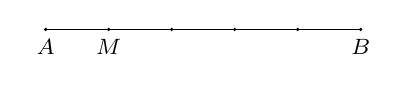
\begin{tikzpicture}[scale=0.8,>=stealth, font=\footnotesize, line join=round, line cap=round]
				\path
					(0,0) coordinate (A) (5,0) coordinate (B)
					(1,0) coordinate (M) (4,0) coordinate (F)
					(3,0) coordinate (P) (2,0) coordinate (T)
				;
				\draw (A)--(B);
				\foreach \a in {A,B,M,F,P,T} \fill[black] (\a)circle(.8pt);
				\foreach \a in {A,B,M} \draw (\a)node[below]{$\a$};
			\end{tikzpicture}
		\end{center}
		\begin{enumerate} [a)]
			\item Thấy $\overrightarrow{AM}$ và $\overrightarrow{AB}$ cùng hướng nên $k>0$. \\
			Ta có $|k|=\dfrac{|\overrightarrow{AM}|}{|\overrightarrow{AB}|}=\dfrac{AM}{AB}=\dfrac{1}{5}$. Suy ra $k=\dfrac{1}{5}$.
			\item Thấy $\overrightarrow{MA}$ và $\overrightarrow{MB}$ ngược hướng nên $k<0$. \\
			Ta có $|k|=\dfrac{|\overrightarrow{MA}|}{|\overrightarrow{MB}|}=\dfrac{AM}{MB}=\dfrac{1}{4}$. Suy ra $k=-\dfrac{1}{4}$.
			\item Thấy $\overrightarrow{MA}$ và $\overrightarrow{AB}$ ngược hướng nên $k<0$. \\
			Ta có $|k|=\dfrac{|\overrightarrow{MA}|}{|\overrightarrow{AB}|}=\dfrac{AM}{AB}=\dfrac{1}{5}$. Suy ra $k=-\dfrac{1}{5}$.
	\end{enumerate}}
\end{bt}

\begin{bt}%[0H1B3-3]
	Cho hai điểm phân biệt $A,B$. Xác định điểm $M$ biết $2\overrightarrow{MA}-3\overrightarrow{MB}=\overrightarrow{0}$.
	\loigiai{
		Ta có
		$2\overrightarrow{MA}-3\overrightarrow{MB}=\overrightarrow{0}\Leftrightarrow 2\overrightarrow{MA}-3(\overrightarrow{MA}+\overrightarrow{AB})=\overrightarrow{0}\Leftrightarrow-\overrightarrow{MA}-3\overrightarrow{AB}=\overrightarrow{0}\Leftrightarrow\overrightarrow{AM}=3\overrightarrow{AB}$ \\
		$ \Rightarrow\overrightarrow{AM},\overrightarrow{AB} $ cùng hướng và $AM=3AB$.
		\begin{center}
			\begin{tikzpicture}[scale=0.8,>=stealth, font=\footnotesize, line join=round, line cap=round]
				\tkzDefPoints{0/0/A,2/0/B,6/0/M,4/0/H}
				\tkzDrawPoints[fill=black,size=5](A,B,M,H)
				\tkzDrawSegments(A,M)
				\tkzLabelPoints[below](A,B,M)
			\end{tikzpicture}
		\end{center}
	}
\end{bt}

\begin{dang}{Tìm mô-đun (độ dài) vectơ}

		\textbf{Phương pháp giải:} Để tính $\left|\overrightarrow{a}\pm \overrightarrow{b}\pm\overrightarrow{c} \pm\overrightarrow{d} \right|$ ta thực hiện theo hai bước sau:
		\begin{enumerate}[Bước 1.]
			\item Biến đổi và rút gọn biểu thức véctơ $\overrightarrow{a}\pm \overrightarrow{b}\pm\overrightarrow{c} \pm\overrightarrow{d}=\overrightarrow{v}$ dựa vào qui tắc ba điểm, tính chất trung điểm, hình bình hành, trọng tâm,.... sao cho $\overrightarrow{v}$ là đơn giản nhất.
			\item Tính độ dài (mô-đun) của $\overrightarrow{v}$ dựa vào tính chất hình học đã cho.
		\end{enumerate}
		\begin{note}
			\centerline{\textbf{Một số kiến thức hình học phẳng thường được sử dụng}}
			\begin{itemize}
				\item Chiều cao tam giác đều $=\text{cạnh}\cdot \dfrac{\sqrt{3}}{2}$.
				\item Đường chéo hình vuông $=\text{cạnh}\cdot \sqrt{2}$.
			\end{itemize}
			Cho tam giác $ABC$ vuông tại $A$, có $AH$ là đường cao, $AM$ là trung tuyến. Khi đó:
			\immini{
				\begin{itemize}
					\item Pitago: $BC^2=AB^2+AC^2\\
					\Rightarrow \heva{&BC=\sqrt{AB^2+AC^2}\\&AB=\sqrt{BC^2-AC^2}\\&AC=\sqrt{BC^2-AB^2.}}$
					\item Trung tuyến $AM=\dfrac{1}{2}BC$.
					\item $AB^2=BH\cdot BC$ và $AC^2=CH\cdot BC$.
				\end{itemize}}
			{\begin{tikzpicture}[scale=0.9, font=\footnotesize,
					line join=round, line cap=round, >=stealth]
					\path
					(0,0) node[left]{$B$} coordinate (B)
					(5,0) node[right]{$C$} coordinate (C)
					($(B)!(C)!(53.13:1cm)$) node[above]{$A$} coordinate (A)
					($(B)!(A)!(C)$) node[below]{$H$} coordinate (H)
					($(B)!0.5!(C)$) node[below]{$M$} coordinate (M);
					\draw (A) -- (B) -- (C) -- cycle;
					\draw (M) -- (A) -- (H);
					\foreach \i in {A,B,C,H,M}
					\fill[black] (\i) circle (1pt);
					\newcommand{\gocv}[4][black]{\draw[#1] ($(#3)!5pt!(#2)$)--($(#3)!2!($($(#3)!5pt!(#2)$)!.5!($(#3)!5pt!(#4)$)$)$)--($(#3)!5pt!(#4)$);}
					\gocv{B}{A}{C}
					\gocv{A}{H}{B}
					\tkzMarkSegments[mark=||](A,M M,B M,C)
					\tkzMarkAngles[size=.4](C,B,A)
			\end{tikzpicture}}
			\begin{itemize}
				\item $\dfrac{1}{HA^2}=\dfrac{1}{AB^2}+\dfrac{1}{AC^2}$ và $AH^2=HB\cdot HC$.
				\item $\sin\widehat {ABC}=\dfrac{\text{đối}}{\text{huyền}}=\dfrac{AC}{BC}$; \qquad
				$\cos\widehat {ABC}=\dfrac{\text{kề}}{\text{huyền}}=\dfrac{AB}{BC}$; \qquad  $\tan\widehat {ABC}=\dfrac{\text{đối}}{\text{kề}}=\dfrac{AC}{AB}$.
			\end{itemize}
		\end{note}

\end{dang}

\begin{bt}%[0H1B3-1]
	Cho tam giác $ABC$ vuông tại $A$, có $AB=3$ cm, $AC=4$ cm. Gọi $I$ là trung điểm $BC$. Xác định và tính độ dài vectơ
		\begin{listEX}[2]
		\item $\overrightarrow{u}=\overrightarrow{BA}+\overrightarrow{BC}$. \dapso{$2\sqrt{3}$ cm.}
		\item $\overrightarrow{v}=\overrightarrow{AB}+\overrightarrow{AC}$. \dapso{$5$ cm.}
		\item $\overrightarrow{w}=\overrightarrow{CA}+\overrightarrow{CB}$. \dapso{$\sqrt{73}$ cm.}
		\item $\overrightarrow{x}=2\overrightarrow{IA}-\overrightarrow{CA}$. \dapso{$3$ cm.}
	\end{listEX}
	\loigiai{
		\begin{enumerate}
			\immini[thm]{
				\item[a)] $\overrightarrow{u}=\overrightarrow{BA}+\overrightarrow{BC}$.\\
				Gọi $M$ là trung điểm của $AC$, ta có\\
				$\overrightarrow{u}=\overrightarrow{BA}+\overrightarrow{BC}=2\overrightarrow{BM}\\
				\Rightarrow \left|\overrightarrow{u}\right|=\left|2\overrightarrow{BM}\right|=2\left|\overrightarrow{BM}\right|=2BM$.\\
				Ta có $MA=2\Rightarrow MB=\sqrt{3^2+2^2}=\sqrt{13}$.\\
				$\Rightarrow \left|\overrightarrow{u}\right|=2BM=2\sqrt{13}$ cm.}
			{\begin{tikzpicture}[scale=1, font=\footnotesize,
					line join=round, line cap=round, >=stealth]
					\tikzset{label style/.style={font=\footnotesize}}
					\tkzDefPoints{0/0/A,3/0/B,0/4/C}
					\coordinate (E) at (-0.5,4);
					\coordinate (F) at (-0.5,0);
					\coordinate (I) at ($(B)!0.5!(C)$);
					\coordinate (M) at ($(A)!0.5!(C)$);
					\coordinate[label=left:{$4$cm}] (K) at ($(E)!0.5!(F)$);
					\draw (A)--(C);
					\draw[->] (B)--(C);
					\draw[->] (B)--(M);
					\draw[->] (B)--(A);
					\draw[<->] (E)--(F);
					\tkzMarkRightAngles[size=0.2](B,A,C)
					\coordinate[label=below:{$J$}] (J) at ($(A)!0.5!(B)$);
					\draw (J)--(C) (A)--(I);
					\tkzDrawPoints[size=2,fill=black](A,B,C,M,I,J)
					\tkzLabelPoints[left](M,A)
					\tkzLabelPoints[above](C)
					\tkzLabelPoints[right](I,B)
					\coordinate[label=above left:{$3$cm}] (K) at ($(A)!0.5!(B)$);
			\end{tikzpicture}}
		\end{enumerate}
			\begin{enumerate}
			\item[b)] $\overrightarrow{w}=\overrightarrow{CA}+\overrightarrow{CB}$. \\
			Gọi $J$ là trung điểm của $AB$, ta có:\\
			$\overrightarrow{w}=\overrightarrow{CA}+\overrightarrow{CB}=2\overrightarrow{CJ}\Rightarrow \left|\overrightarrow{w}\right|=\left|2\overrightarrow{CJ}\right|=2\left|\overrightarrow{CJ}\right|=2CJ$.\\
			Ta có $AJ=\dfrac{3}{2}\Rightarrow CJ=\sqrt{4^2+{\dfrac{3}{2}}^2}=\dfrac{\sqrt{73}}{2}$.\\
			$\Rightarrow \left|\overrightarrow{w}\right|=2CJ=\sqrt{73}$ cm.
			\item[c)] $\overrightarrow{x}=2\overrightarrow{IA}-\overrightarrow{CA}$.\\
			Ta có $\overrightarrow{x}=2\overrightarrow{IA}-\overrightarrow{CA}=2\overrightarrow{IA}+\overrightarrow{AC}=2\overrightarrow{IA}+2\overrightarrow{AM}=2\left(\overrightarrow{IA}+\overrightarrow{AM} \right)=2\overrightarrow{IM}$.\\
			$\Rightarrow \left|\overrightarrow{x}\right|=\left|2\overrightarrow{IM}\right|=2IM=AB=3$ cm.
		\end{enumerate}
	}
\end{bt}
\begin{bt}%[0H1B3-1]
	Cho tam giác $ABC$ đều cạnh $a$, gọi $G$ là trọng tâm tam giác và $H$ là trung điểm $BC$. Tính
	\begin{listEX}[2]
		\item $\left|\overrightarrow{AB}+\overrightarrow{AC}\right|$. \dapso{$a\sqrt{3}$.}
		\item $\left|\overrightarrow{AB}-\overrightarrow{AC}\right|$. \dapso{$a$.}
		\item $\left|\overrightarrow{GA}-\overrightarrow{GC}\right|$. \dapso{$a$.}
		\item $\left|\overrightarrow{GB}+\overrightarrow{GC}\right|$. \dapso{$\dfrac{a\sqrt{3}}{3}$.}
		\item $\left|\overrightarrow{AH}+\overrightarrow{BC}\right|$. \dapso{$\dfrac{a\sqrt{7}}{2}$.}
	\end{listEX}
	\loigiai{
		Ta có tam giác $ABC$ đều cạnh $a$ suy ra $AH=\dfrac{a\sqrt{3}}{2}$, $AG=\dfrac{2}{3}AH=\dfrac{a\sqrt{3}}{3}$, $GH=\dfrac{1}{3}AH=\dfrac{a\sqrt{3}}{6}$.\\
		\begin{listEX}
			\immini[thm]{
				\item[a)] $\left|\overrightarrow{AB}+\overrightarrow{AC}\right|$.\\
				Ta có $\overrightarrow{AB}+\overrightarrow{AC}=2\overrightarrow{AH}$.\\
				$\Rightarrow \left|\overrightarrow{AB}+\overrightarrow{AC}\right|=\left|2\overrightarrow{AH}\right|=2AH=2\cdot\dfrac{a\sqrt{3}}{2}=a\sqrt{3}$.
				\item[b)] $\left|\overrightarrow{AB}-\overrightarrow{AC}\right|$.\\
				Ta có  $\left|\overrightarrow{AB}-\overrightarrow{AC}\right|=\left|\overrightarrow{CB}\right|=a$.
				\item[c)] $\left|\overrightarrow{GA}-\overrightarrow{GC}\right|$.\\
				Ta có $\left|\overrightarrow{GA}-\overrightarrow{GC}\right|=\left|\overrightarrow{CA}\right|=CA=a$.}
			{\begin{tikzpicture}[scale=1, font=\footnotesize,
					line join=round, line cap=round, >=stealth]
					\tikzset{label style/.style={font=\footnotesize}}
					\tkzDefPoints{0/0/B,4/0/C}
					\tkzDefEquilateral(B,C)\tkzGetPoint{A}
					\draw (A)--(B)--(C)--cycle;
					\tkzCentroid(A,B,C)\tkzGetPoint{G}
					\coordinate[label=below:{$H$}] (H) at ($(C)!0.5!(B)$);
					\coordinate[label=left:{$M$}] (M) at ($(H)!0.5!(A)$);
					\coordinate (K) at ($(C)!0.5!(A)$);
					\draw (A)--(H) (C)--(G) (B)--(K) (M)--(C);
					\tkzDrawPoints[size=2,fill=black](A,B,C,H,G,K,M)
					\tkzLabelPoints[left](B,G)
					\tkzLabelPoints[above](A)
					\tkzLabelPoints[right](C)
			\end{tikzpicture}}
			\item[d)] $\left|\overrightarrow{GB}+\overrightarrow{GC}\right|$.\\
			Ta có $\overrightarrow{GB}+\overrightarrow{GC}=2\overrightarrow{GH}$.\\
			$\Rightarrow \left|\overrightarrow{GB}+\overrightarrow{GC}\right|=\left|2\overrightarrow{GH}\right|=2GH=\dfrac{a\sqrt{3}}{3}$.
			\item[e)] $\left|\overrightarrow{AH}+\overrightarrow{BC}\right|$.\\
			Gọi $M$ là trung điểm của $AH$.\\
			Ta có $\overrightarrow{AH}+\overrightarrow{BC}=\overrightarrow{BC}-\overrightarrow{HA}=2\overrightarrow{HC}-2\overrightarrow{HM}=2\left(\overrightarrow{HC}-\overrightarrow{HM}\right)=2\overrightarrow{MC}$.\\
			Ta có $MH=\dfrac{1}{2}AH=\dfrac{a\sqrt{3}}{4}$, $HC=\dfrac{a}{2}\\
			\Rightarrow MC=\sqrt{HM^2+HC^2}=\sqrt{\left(\dfrac{a\sqrt{3}}{4}\right)^2+\left(\dfrac{a}{2}\right)^2}=\dfrac{a\sqrt{7}}{4}$.\\
			$\Rightarrow \left|\overrightarrow{AH}+\overrightarrow{BC}\right|=\left|2\overrightarrow{MC}\right|=2\left|\overrightarrow{MC}\right|=2MC=2\cdot \dfrac{a\sqrt{7}}{4}=\dfrac{a\sqrt{7}}{2}$.
		\end{listEX}
	}
\end{bt}
\begin{bt}%[0H1B3-1]
	Cho hình chữ nhật $ABCD$ có $AB=3$, $BC=4$. Gọi $M$, $N$ lần lượt là trung điểm của $BC$ và $CD$. Tính
	\begin{listEX}[2]
		\item $\left|\overrightarrow{AB}+\overrightarrow{AC}+\overrightarrow{AD}\right|$. \dapso{$10$.}
		\item $\left|\overrightarrow{AM}+\overrightarrow{AN}\right|$. \dapso{$\dfrac{15}{2}$.}
	\end{listEX}
	\loigiai{
		\begin{listEX}
			\immini[thm]{
				\item[a)] Ta có
				\allowdisplaybreaks
				\begin{eqnarray*}
					\left|\overrightarrow{AB}+\overrightarrow{AC}+\overrightarrow{AD}\right|&=&\left|\left(\overrightarrow{AB}+\overrightarrow{AD}\right)+\overrightarrow{AC}\right|\\
					&=&\left|\overrightarrow{AC}+\overrightarrow{AC}\right|	\\
					&=&\left|2\overrightarrow{AC}\right|\\
					&=&2AC=2\cdot\sqrt{3^2+4^2}=10
			\end{eqnarray*}}
			{\begin{tikzpicture}[scale=1, font=\footnotesize,
					line join=round, line cap=round, >=stealth]
					\tikzset{label style/.style={font=\footnotesize}}
					\coordinate[label=left:{$B$}] (B) at (0,0);
					\coordinate[label=left:{$A$}] (A) at (0,3);
					\coordinate[label=right:{$D$}] (D) at (4,3);
					\coordinate[label=right:{$C$}] (C) at (4,0);
					\coordinate[label=below:{$M$}] (M) at ($(C)!0.5!(B)$);
					\coordinate[label=right:{$N$}] (N) at ($(C)!0.5!(D)$);
					\coordinate[label=above:{$4$}] (K) at ($(A)!0.5!(D)$);
					\coordinate[label=left:{$3$}] (H) at ($(A)!0.5!(B)$);
					\coordinate[label=below:{$E$}] (E) at ($(M)!0.5!(N)$);
					\coordinate[label=left:{$O$}] (O) at ($(A)!0.5!(C)$);
					\draw (A)--(B)--(C)--(D)--cycle;
					\draw (A)--(M) (A)--(N) (M)--(N) (B)--(D) (A)--(C) (M)--(O)--(N);
					\tkzDrawPoints[size=2,fill=black](A,B,C,D,M,N,O,E)
					\newcommand{\gocv}[4][black]{\draw[#1] ($(#3)!5pt!(#2)$)--($(#3)!2!($($(#3)!5pt!(#2)$)!.5!($(#3)!5pt!(#4)$)$)$)--($(#3)!5pt!(#4)$);}
					\gocv{B}{A}{D}
					\gocv{A}{D}{C}
					\gocv{B}{C}{D}
					\gocv{A}{B}{C}
			\end{tikzpicture}}
			\item $\left|\overrightarrow{AM}+\overrightarrow{AN}\right|$.\\
			Gọi $O=AC\cap BD$, $E=AC\cap MN$.\\
			Ta có tứ giác $MONC$ là hình chữ nhật, có $E$ là trung điểm của $OC$ (đường trung bình) suy ra $E$ là trung điểm của $MN$.\\
			$\Rightarrow \left|\overrightarrow{AM}+\overrightarrow{AN}\right|=\left|2\overrightarrow{AE}\right|=2AE=2(AC-CE)$.\\
			Do $AC=\sqrt{3^2+4^2}=5$, $CE=\dfrac{1}{2}MN=\dfrac{1}{4}BD=\dfrac{1}{4}AC=\dfrac{5}{4}$.\\
			$\Rightarrow \left|\overrightarrow{AM}+\overrightarrow{AN}\right|=2(AC-CE)=2\left(5-\dfrac{5}{4}\right)=\dfrac{15}{2}$.
		\end{listEX}
	}
\end{bt}



\begin{dang}{Chứng minh ba điểm $M, N, P$ thẳng hàng}
	Để chứng minh ba điểm $M, N, P$ thẳng hàng ta chọn một điểm làm điểm gốc, giả sử chọn điểm $ M $. Sau đó  chứng minh một trong hai đẳng thức sau  $$\overrightarrow{MN}=k\overrightarrow{MP} \text{ với } k\neq 0.$$
	$$\overrightarrow{MP}=k\overrightarrow{MN} \text{ với } k\neq 0.$$
\end{dang}

\begin{bt}%[0H1K3-5]
	Cho tam giác $ABC$ có trung tuyến $AM$. Gọi $I$ là trung điểm $AM$ và $K$ là  điểm thuộc $AC$ sao $AK=\dfrac{1}{3}AC$. Chứng minh ba điểm $B, I, K$ thẳng hàng.
	\loigiai{
		\immini
		{
			Ta có $2\overrightarrow{BI}=\overrightarrow{BA}+\overrightarrow{BM}=\overrightarrow{BA}+\dfrac{1}{2}\overrightarrow{BC}$ \\
			$\Rightarrow 4\overrightarrow{BI}=2\overrightarrow{BA}+\overrightarrow{BC}$. $\quad(1)$\\
			Ta có
			\allowdisplaybreaks
			\begin{eqnarray*}
				\overrightarrow{BK}&=&\overrightarrow{BA}+\overrightarrow{AK} \\
				&=&\overrightarrow{BA}+\dfrac{1}{3}\overrightarrow{AC} \\ &=&\overrightarrow{BA}+\dfrac{1}{3}(\overrightarrow{BC}-\overrightarrow{BA}) \\
				&=&\dfrac{2}{3}\overrightarrow{BA}+\dfrac{1}{3}\overrightarrow{BC}.
			\end{eqnarray*}
			Suy ra $3\overrightarrow{BK}=2\overrightarrow{BA}+\overrightarrow{BC}$. $\quad(2) $
		}
		{
			\begin{tikzpicture}[font=\scriptsize,scale=0.7]
				\path
				(0,0) coordinate (B)
				(1,3)  coordinate (A)
				(5,0) coordinate (C);
				\coordinate (M) at ($(B)!.5!(C)$);
				\coordinate (I) at ($(A)!.5!(M)$);
				\coordinate (K) at (intersection of B--I and A--C);

				\draw (A)--(B)--(C)--cycle	(B)--(K) (A)--(M);
				\foreach \x/\g in {A/90, B/250,C/270,M/270,I/0,K/0}
				\fill[black](\x) circle (1.5pt) ($(\x)+(\g:4mm)$)node{\x};
				\draw (A)--(I)node[midway,rotate=-20]{$||$} (I)--(M)node[midway,rotate=-20]{$||$}; % Đánh dấu kí hiệu || chính giữa đoạn thẳng AB
			\end{tikzpicture}
		}
	\noindent
	Từ $(1)$ và $(2)$ suy ra $3\overrightarrow{BK}=4\overrightarrow{BI}\Rightarrow\overrightarrow{BK}=\dfrac{4}{3}\overrightarrow{BI}\Rightarrow B, I, K$ thẳng hàng.
	}
\end{bt}
\begin{bt}%[0H1K3-5]
	Cho tam giác $ABC$. Hai điểm $M, N$ được xác định bởi hệ thức
	$\overrightarrow{BC}+\overrightarrow{MA}=\overrightarrow{0}$,  $\overrightarrow{AB}-\overrightarrow{NA}-3\overrightarrow{AC}=\overrightarrow{0}$. Chứng minh $MN\parallel AC$.
	\loigiai{
		Ta có $\overrightarrow{BC}+\overrightarrow{MA}+\overrightarrow{AB}-\overrightarrow{NA}-3\overrightarrow{AC}=\overrightarrow{0}$ hay $\overrightarrow{AC}+\overrightarrow{MN}-3\overrightarrow{AC}=\overrightarrow{0}\Leftrightarrow\overrightarrow{MN}=2\overrightarrow{AC}$.\\
		Vậy $\overrightarrow{MN},\overrightarrow{AC}$ cùng phương.\\
		Theo giả thiết $\overrightarrow{BC}=\overrightarrow{AM}$. Mà $A,B,C$ không thẳng hàng nên bốn điểm $A,B,C,M$ là bốn đỉnh của hình bình hành suy ra $M$ không thuộc $AC$.\\
		Vậy $MN\parallel AC$.}
\end{bt}

\begin{dang}{Biểu diễn vectơ qua hai vectơ không cùng phương}
	Cho hai vectơ không cùng phương $\overrightarrow{a}$ và $\overrightarrow{b}$. Khi đó với mọi vectơ $\overrightarrow{c}$ ta có duy nhất một cách biểu diễn sau
		$$\overrightarrow{c} = m\overrightarrow{a} + n\overrightarrow{b}.$$
	Ta thường sử dụng các quy tắc
	\begin{enumerate}[+]
		\item Quy tắc ba điểm $\overrightarrow{MN} = \overrightarrow{MO} + \overrightarrow{ON} = \overrightarrow{ON} - \overrightarrow{OM}$.
		\item Quy tắc trung điểm $\overrightarrow{OM} = \dfrac{1}{2}\left(\overrightarrow{OA}+\overrightarrow{OB}\right)$.
		\item Quy tắc hình bình hành $\overrightarrow{AB}+\overrightarrow{AD} = \overrightarrow{AC} = 2\overrightarrow{AO}$ với $ABCD$ là hình bình hành tâm $O$.
	\end{enumerate}
	\begin{center}
		\begin{tikzpicture}[scale=1, line cap=round, line join=round, font=\footnotesize, >=stealth]
		\path
			(0,0) coordinate (O) (-1,2) coordinate (A) (3,2) coordinate (B)
			($(A)!.5!(B)$) coordinate (M)
		;
		\foreach \a in {A,B,M}{\draw[->] (O)--(\a);}
		\draw (A)--node[pos=.5, rotate=-30]{|}(M)--node[pos=.5, rotate=-30]{|}(B);
		\foreach \a/\b in {O/-90,A/180,B/0,M/90} \fill[black] (\a) circle(.5pt) ($(\a)+(\b:3mm)$)node{$\a$};
	\end{tikzpicture} \quad
	\begin{tikzpicture}[scale=1, line cap=round, line join=round, font=\footnotesize, >=stealth]
		\path
		(0,0) coordinate (A) (4,-1) coordinate (B) (1,1.5) coordinate (D)
		($(D)!.5!(B)$) coordinate (O) ($(O)!-1!(A)$) coordinate (C)
		;
		\foreach \a in {D,B,C,O}{\draw[->] (A)--(\a);}
		\draw (B)--(C)--(D)--cycle;
		\foreach \a/\b in {O/-90,A/180,B/0,C/60,D/90} \fill[black] (\a) circle(.5pt) ($(\a)+(\b:3mm)$)node{$\a$};
	\end{tikzpicture}
	\end{center}
\end{dang}

\begin{bt}%[0H1K3-4]
	Cho tam giác $ABC$. Gọi $M$ là một điểm trên cạnh $BC$ sao cho $MB=2MC$. Chứng minh rằng $\overrightarrow{AM}=\dfrac{1}{3}\overrightarrow{AB}+\dfrac{2}{3}\overrightarrow{AC}$.
	\loigiai{

		\immini
		{
			Ta có
			\allowdisplaybreaks
			\begin{eqnarray*}
				\overrightarrow{AM}
				&=&\overrightarrow{AC}+\overrightarrow{CM}=\overrightarrow{AC}-\dfrac{1}{3}\overrightarrow{BC}\\&=&\overrightarrow{AC}-\dfrac{1}{3}(\overrightarrow{AC}-\overrightarrow{AB})=\dfrac{1}{3}\overrightarrow{AB}+\dfrac{2}{3}\overrightarrow{AC}\text{ (đpcm)}.
			\end{eqnarray*}
		}
		{
			\begin{tikzpicture}[font=\scriptsize,scale=0.7]
				\path
				(0,0) coordinate (B)
				(1,3)  coordinate (A)
				(6,0) coordinate (C);
				\coordinate (M) at (4,0);
				\draw (B)--(C);
				\foreach \x/\g in{A/B,A/M,A/C}
				\draw[-stealth] (\x)--(\g);
				\foreach \x/\g in {A/90, B/250,C/270,M/270}
				\fill[black](\x) circle (1.5pt) ($(\x)+(\g:4mm)$)node{\x};
			\end{tikzpicture}
		}
	}
\end{bt}

\begin{bt}%[0H1K3-4]
	Cho $\triangle ABC$ có trọng tâm $G$. Cho các điểm $D, E, F$ lần lượt là trung điểm của các cạnh $BC, CA, AB$ và $I$ là giao điểm của $AD$ và $EF$. Đặt $\overrightarrow{u}=\overrightarrow{AE},\overrightarrow{v}=\overrightarrow{AF}$. Hãy phân tích các vectơ $\overrightarrow{AI}$, $\overrightarrow{AG}$, $\overrightarrow{DE}$, $\overrightarrow{DC}$ theo hai vectơ $\overrightarrow{u}$ và $\overrightarrow{v}$.
	\loigiai{
		\immini
		{
			Ta có $AEDF$ là hình bình hành \\
			$\Rightarrow\overrightarrow{AD}=\overrightarrow{AE}+\overrightarrow{AF}$.\\
			Do đó
			\begin{itemize}
				\item $\overrightarrow{AI}=\dfrac{1}{2}\overrightarrow{AD}=\dfrac{1}{2}(\overrightarrow{AE}+\overrightarrow{AF})=\dfrac{1}{2}(\overrightarrow{u}+\overrightarrow{v})$.
				\item $\overrightarrow{AG}=\dfrac{2}{3}\overrightarrow{AD}=\dfrac{2}{3}(\overrightarrow{AE}+\overrightarrow{AF})=\dfrac{2}{3}(\overrightarrow{u}+\overrightarrow{v})$.
				\item $\overrightarrow{DE}=\overrightarrow{FA}=-\overrightarrow{AF}=0\cdot\overrightarrow{u}+(-1)\overrightarrow{v}$.
				\item $\overrightarrow{DC}=\overrightarrow{FE}=\overrightarrow{AE}-\overrightarrow{AF}=\overrightarrow{u}-\overrightarrow{v}$.
			\end{itemize}
		}
		{
			\begin{tikzpicture}[font=\scriptsize]
				\path
				(0,0) coordinate (B)
				(1,3)  coordinate (A)
				(6,0) coordinate (C);
				\coordinate (F) at ($(A)!.5!(B)$);
				\coordinate (E) at ($(A)!.5!(C)$);
				\coordinate (D) at ($(C)!.5!(B)$);
				\draw (A)--(B)--(C)--cycle (D)--(E)--(F)--cycle;
				\draw (A)--(D)coordinate[pos=2/3](G) ;
				\coordinate (I) at (intersection of A--D and E--F);
				\foreach \x/\g in{A/F,A/E}
				\draw[-stealth] (\x)--(\g);
				\foreach \x/\g in {A/90, B/250,C/270,D/270,E/90,F/180,G/0,I/90}
				\fill[black](\x) circle (1.5pt) ($(\x)+(\g:4mm)$)node{\x};
			\end{tikzpicture}
		}
	}
\end{bt}

\begin{bt}%[0H1K3-4]
	Cho $AK$ và $BM$ là hai trung tuyến của tam giác $ABC$, trọng tâm $G$. Hãy phân tích các vectơ $\overrightarrow{AB}$, $\overrightarrow{BC}$ theo hai vectơ $\overrightarrow{u}=\overrightarrow{AK}$, $\overrightarrow{v}=\overrightarrow{BM}$.
	\loigiai{
		\immini
		{ Ta có
			\begin{itemize}
				\item $\overrightarrow{AB}=\overrightarrow{AG}+\overrightarrow{GB}=\dfrac{2}{3}\overrightarrow{AK}-\dfrac{2}{3}\overrightarrow{BM} =\dfrac{2}{3}\overrightarrow{u}-\dfrac{2}{3}\overrightarrow{v}$.
				\item $\overrightarrow{BC}=2\overrightarrow{BK}=2\left(\overrightarrow{BG}+\overrightarrow{GK}\right)=2\cdot\dfrac{2}{3}\overrightarrow{BM}+\dfrac{2}{3}\overrightarrow{AK}$ \\
				\hspace*{0.65cm} $=\dfrac{2}{3}\overrightarrow{AK}+\dfrac{4}{3}\overrightarrow{BM}=\dfrac{2}{3}\overrightarrow{u}+\dfrac{4}{3}\overrightarrow{v}$.
			\end{itemize}
		}
		{
			\begin{tikzpicture}[font=\scriptsize,scale=0.7]
				\path
				(0,0) coordinate (B)
				(1,3)  coordinate (A)
				(6,0) coordinate (C);
				\coordinate (K) at ($(B)!.5!(C)$);
				\coordinate (M) at ($(A)!.5!(C)$);
				\coordinate (G) at (intersection of A--K and B--M);
				\draw (A)--(B)--(C)--cycle (A)--(K) (B)--(M);
				\foreach \x/\g in {A/90, B/250,C/270,M/90,K/260,G/270}
				\fill[black](\x) circle (1.5pt) ($(\x)+(\g:4mm)$)node{\x};
			\end{tikzpicture}
	}}
\end{bt}

\begin{dang}{Chứng minh đẳng thức vectơ}
	Để chứng minh đẳng thức vectơ, ta thường thực hiện theo một trong các cách sau.
	\begin{enumerate}[\bfseries Cách 1.]
		\item Biến đổi vế trái sao cho xuất hiện lần lượt các đối tượng ở vế phải.
		\item Biến đổi vế phải sao cho xuất hiện lần lượt các đối tượng ở vế trái.
		\item Xét hiệu $VT-VP=\ldots =\ldots = \overrightarrow{0}$.
		\item Chứng minh hai vế cùng bằng một biểu thức thứ ba.
	\end{enumerate}
	Thường áp dụng các quy tắc: Quy tắc ba điểm; Quy tắc tổng hiệu vectơ; Quy tắc trung điểm; Quy tắc HBH; Quy tắc trọng tâm...
\end{dang}
%Bài tập bổ sung
\begin{bt}%[0H1B1-3]
	Cho 5 điểm $A,B,C,D,E$. Chứng minh rằng
	\begin{enumerate}
		\item $\overrightarrow{AB}+\overrightarrow{CD}+\overrightarrow{EA}=\overrightarrow{CB}+\overrightarrow{ED}$.
		\item $\overrightarrow{CD}+\overrightarrow{EA}=\overrightarrow{CA}+\overrightarrow{ED}$.
	\end{enumerate}
	\loigiai{
		\begin{enumerate}
			\item 	Biến đổi vế trái theo vế phải
			\begin{eqnarray*}
				\text{Vế trái}
				&=&\overrightarrow{AB}+\overrightarrow{CD}+\overrightarrow{EA}\\
				&=&\left(\overrightarrow{AC}+\overrightarrow{CB}\right)+\overrightarrow{CD}+\left(\overrightarrow{ED}+\overrightarrow{DA}\right)\\
				&=&\left(\overrightarrow{CA}+\overrightarrow{ED}\right)+\left(\overrightarrow{AD}+\overrightarrow{DA}\right)\\
				&=&\overrightarrow{CB}+\overrightarrow{ED}+\left(\overrightarrow{AD}+\overrightarrow{DA}\right)\\
				&=&\overrightarrow{CB}+\overrightarrow{ED}+\left(\overrightarrow{AD}-\overrightarrow{AD}\right)\\
				&=&\overrightarrow{CB}+\overrightarrow{ED}=\text{vế phải (đpcm).}
			\end{eqnarray*}
			Cách 2. Biến đổi vế phải theo vế trái.
			\begin{eqnarray*}
				\text{Vế phải}
				&=&\overrightarrow{CB}+\overrightarrow{ED}\\
				&=&\left(\overrightarrow{CA}+\overrightarrow{AB}\right)+\left(\overrightarrow{EA}+\overrightarrow{AD}\right)\\
				&=&\overrightarrow{AB}+\left(\overrightarrow{CA}+\overrightarrow{AD}\right)+\overrightarrow{EA}\\
				&=&\overrightarrow{AB}+\overrightarrow{CD}+\overrightarrow{EA}=\text{vế trái (đpcm).}
			\end{eqnarray*}
			Cách 3. Giả sử ta luôn có:
			\begin{eqnarray*}
				&  &\overrightarrow{AB}+\overrightarrow{CD}+\overrightarrow{EA}=\overrightarrow{CB}+\overrightarrow{ED}\\
				&\Leftrightarrow& \overrightarrow{AB}+\left(\overrightarrow{CD}-\overrightarrow{CB}\right)+\left(\overrightarrow{EA}-\overrightarrow{ED}\right)=\overrightarrow{0}\\
				&\Leftrightarrow& \overrightarrow{AB}+\overrightarrow{BD}+\overrightarrow{DB}=\overrightarrow{0}\\
				&\Leftrightarrow& \overrightarrow{AB}+\overrightarrow{DA}=\overrightarrow{0}\\
				&\Leftrightarrow& \overrightarrow{0}=\overrightarrow{0} (\text{luôn đúng})
			\end{eqnarray*}

			Suy ra  $\overrightarrow{AB}+\overrightarrow{CD}+\overrightarrow{EA}=\overrightarrow{CB}+\overrightarrow{ED}$
			\item Biến đổi vế trái theo vế phải
			\begin{eqnarray*}
				\text{Vế trái}
				&=&\overrightarrow{CD}+\overrightarrow{EA}\\
				&=&\left(\overrightarrow{CA}+\overrightarrow{AD}\right)+\left(\overrightarrow{ED}+\overrightarrow{DA}\right)\\
				&=&\left(\overrightarrow{CA}+\overrightarrow{ED}\right)+\left(\overrightarrow{AD}+\overrightarrow{DA}\right)\\
				&=&\left(\overrightarrow{CA}+\overrightarrow{ED}\right)+\overrightarrow{AA}	\\
				&=&\overrightarrow{CA}+\overrightarrow{ED}=\text{vế phải (đpcm).}
			\end{eqnarray*}
			Cách 2. Biến đổi vế phải theo vế trái.
			\begin{eqnarray*}
				\text{Vế phải}
				&=&\overrightarrow{CA}+\overrightarrow{ED}\\
				&=&\left(\overrightarrow{CD}+\overrightarrow{DA}\right)+\left(\overrightarrow{EA}+\overrightarrow{AD}\right)\\
				&=&\left(\overrightarrow{CD}+\overrightarrow{EA}\right)+\overrightarrow{DA}+\overrightarrow{AD}\\
				&=&\left(\overrightarrow{CD}+\overrightarrow{EA}\right)+\overrightarrow{DD}\\
				&=&\left(\overrightarrow{CD}+\overrightarrow{EA}\right)+\overrightarrow{0}\\
				&=&\overrightarrow{CD}+\overrightarrow{EA}=\text{vế trái (đpcm).}
			\end{eqnarray*}
			Cách 3. Giả sử ta luôn có:
			\begin{eqnarray*}
				& &\overrightarrow{CD}+\overrightarrow{EA}=\overrightarrow{CA}+\overrightarrow{ED}\\
				&\Leftrightarrow& \overrightarrow{CD}-\overrightarrow{CA}+\overrightarrow{EA}-\overrightarrow{ED}=\overrightarrow{0}\\
				&\Leftrightarrow& \overrightarrow{AD}+\overrightarrow{DA}=\overrightarrow{0}\\
				& \Leftrightarrow& \overrightarrow{AA}=\overrightarrow{0}\\
				&\Leftrightarrow &\overrightarrow{0}=\overrightarrow{0} (\text{luôn đúng})
			\end{eqnarray*}
			Suy ra  $\overrightarrow{CD}+\overrightarrow{EA}=\overrightarrow{CA}+\overrightarrow{ED}$
		\end{enumerate}
	}
\end{bt}

\begin{bt}%[0H1B1-3]
	Cho các điểm bất kì. Hãy chứng minh đẳng thức
	\begin{enumerate}
		\item $\overrightarrow{AB}+\overrightarrow{BC}+\overrightarrow{CD}+\overrightarrow{DE}=\overrightarrow{AE}$.
		\item $\overrightarrow{AB}+\overrightarrow{BC}+\overrightarrow{CD}+\overrightarrow{DE}+\overrightarrow{EF}=\overrightarrow{AF}$.
		\item $\overrightarrow{AC}+\overrightarrow{BD}=\overrightarrow{AD}+\overrightarrow{BC}$.
		\item $\overrightarrow{AB}+\overrightarrow{CD}=\overrightarrow{AD}+\overrightarrow{CB}$.
		\item $\overrightarrow{AB}-\overrightarrow{CD}=\overrightarrow{AC}-\overrightarrow{BD}$.
		\item $\overrightarrow{AB}-\overrightarrow{AD}=\overrightarrow{CB}-\overrightarrow{CD}$.
		\item $\overrightarrow{BC}+\overrightarrow{AB}=\overrightarrow{DC}+\overrightarrow{AD}$.
		\item $\overrightarrow{AB}+\overrightarrow{BC}+\overrightarrow{CD}+\overrightarrow{DA}=\overrightarrow{0}$.
		\item $\overrightarrow{AD}+\overrightarrow{BE}+\overrightarrow{CF}=\overrightarrow{AE}+\overrightarrow{BF}+\overrightarrow{CD}$.
		\item $\overrightarrow{AC}+\overrightarrow{DE}-\overrightarrow{DC}-\overrightarrow{CE}+\overrightarrow{CB}=\overrightarrow{AB}$.
	\end{enumerate}
	\loigiai{
		\begin{enumerate}
			\item \begin{eqnarray*}
				\text{Vế trái}
				&=&\overrightarrow{AB}+\overrightarrow{BC}+\overrightarrow{CD}+\overrightarrow{DE}\\
				&=&\overrightarrow{AC}+\overrightarrow{CE}\\
				&=&\overrightarrow{AE}=\text{vế phải}.
			\end{eqnarray*}
			\item \begin{eqnarray*}
				\text{Vế trái}
				&=&\overrightarrow{AB}+\overrightarrow{BC}+\overrightarrow{CD}+\overrightarrow{DE}+\overrightarrow{EF}\\
				&=&\overrightarrow{AC}+\overrightarrow{CE}+\overrightarrow{EF}\\
				&=&\overrightarrow{AE}+\overrightarrow{EF}\\
				&=&\overrightarrow{AF}=\text{vế phải}.
			\end{eqnarray*}
			\item \begin{eqnarray*}
				\text{Vế trái}
				&=&\overrightarrow{AC}+\overrightarrow{BD}\\
				&=&\overrightarrow{AD}+\overrightarrow{DC}+\overrightarrow{BC}+\overrightarrow{CD}\\
				&=&\overrightarrow{AD}+\overrightarrow{BC}+\overrightarrow{DC}+\overrightarrow{CD}\\
				&=&\overrightarrow{AD}+\overrightarrow{BC}+\overrightarrow{DD}\\
				&=&\overrightarrow{AD}+\overrightarrow{BC}=\text{vế phải}.
			\end{eqnarray*}
			\item \begin{eqnarray*}
				\text{Vế trái}
				&=&\overrightarrow{AB}+\overrightarrow{CD}\\
				&=&\overrightarrow{AD}+\overrightarrow{DB}+\overrightarrow{CB}+\overrightarrow{BD}\\
				&=&\overrightarrow{AD}+\overrightarrow{CB}+\overrightarrow{DB}+\overrightarrow{BD}\\
				&=&\overrightarrow{AD}+\overrightarrow{CB}+\overrightarrow{DD}\\
				&=&\overrightarrow{AD}+\overrightarrow{CB}+\overrightarrow{0}\\
				&=&\overrightarrow{AD}+\overrightarrow{CB}=\text{vế phải}.
			\end{eqnarray*}
			\item \begin{eqnarray*}
				\text{Vế trái}
				&=&\overrightarrow{AB}-\overrightarrow{CD}\\
				&=&\overrightarrow{AB}+\overrightarrow{DC}\\
				&=&\overrightarrow{AC}+\overrightarrow{CB}+\overrightarrow{DB}+\overrightarrow{BC}\\
				&=&\overrightarrow{AC}+\overrightarrow{DB}+\overrightarrow{CB}+\overrightarrow{BC}\\
				&=&\overrightarrow{AC}-\overrightarrow{BD}+\overrightarrow{CC}\\
				&=&\overrightarrow{AC}-\overrightarrow{BD}+\overrightarrow{0}\\
				&=&\overrightarrow{AC}-\overrightarrow{BD}=\text{vế phải}.
			\end{eqnarray*}
			\item \begin{eqnarray*}
				& &\overrightarrow{AB}-\overrightarrow{AD}=\overrightarrow{CB}-\overrightarrow{CD}\\
				&\Leftrightarrow& \overrightarrow{DB}=\overrightarrow{DB} (\text{đúng}).\\
				&\text{Vậy}& \overrightarrow{AB}-\overrightarrow{AD}=\overrightarrow{CB}-\overrightarrow{CD}.
			\end{eqnarray*}
			\item \begin{eqnarray*}
				\text{Vế trái}
				&=&\overrightarrow{BC}+\overrightarrow{AB}\\
				&=&\overrightarrow{BD}+\overrightarrow{DC}+\overrightarrow{AD}+\overrightarrow{DB}\\
				&=&\overrightarrow{DC}+\overrightarrow{AD}+\overrightarrow{BD}+\overrightarrow{DB}\\
				&=&\overrightarrow{DC}+\overrightarrow{AD}+\overrightarrow{BB}\\
				&=&\overrightarrow{DC}+\overrightarrow{AD}+\overrightarrow{0}\\
				&=&\overrightarrow{DC}+\overrightarrow{AD}=\text{vế phải}.
			\end{eqnarray*}
			\item \begin{eqnarray*}
				\text{Vế trái}
				&=&\overrightarrow{AB}+\overrightarrow{BC}+\overrightarrow{CD}+\overrightarrow{DA}\\
				&=&\overrightarrow{AC}+\overrightarrow{CA}\\
				&=&\overrightarrow{AA}=\text{vế phải}.
			\end{eqnarray*}
			\item \begin{eqnarray*}
				\text{Vế trái}
				&=&\overrightarrow{AD}+\overrightarrow{BE}+\overrightarrow{CF}\\
				&=&\overrightarrow{AE}+\overrightarrow{ED}+\overrightarrow{BF}+\overrightarrow{FE}+\overrightarrow{CD}+\overrightarrow{DF}\\
				&=&\overrightarrow{AE}+\overrightarrow{BF}+\overrightarrow{CD}+\overrightarrow{ED}+\overrightarrow{FE}+\overrightarrow{DF}\\
				&=&\overrightarrow{AE}+\overrightarrow{BF}+\overrightarrow{CD}+\overrightarrow{ED}+\overrightarrow{DE}\\
				&=&\overrightarrow{AE}+\overrightarrow{BF}+\overrightarrow{CD}+\overrightarrow{EE}\\
				&=&\overrightarrow{AE}+\overrightarrow{BF}+\overrightarrow{CD}=\text{vế phải}.
			\end{eqnarray*}
			\item \begin{eqnarray*}
				\text{Vế trái}
				&=&\overrightarrow{AC}+\overrightarrow{DE}-\overrightarrow{DC}-\overrightarrow{CE}+\overrightarrow{CB}\\
				&=&\overrightarrow{AC}+\overrightarrow{DE}+\overrightarrow{CD}+\overrightarrow{EC}+\overrightarrow{CB}\\
				&=&\overrightarrow{AC}+\overrightarrow{CD}+\overrightarrow{DE}+\overrightarrow{EC}+\overrightarrow{CB}\\
				&=&\overrightarrow{AD}+\overrightarrow{DC}+\overrightarrow{CB}\\
				&=&\overrightarrow{AC}+\overrightarrow{CB}\\
				&=&\overrightarrow{AB}=\text{Vế phải}.
			\end{eqnarray*}
		\end{enumerate}
	}
\end{bt}
%2
\begin{bt}%[0H1B1-3]
	Cho tứ giác lồi $ABCD$. Gọi $I$, $J$ lần lượt là trung điểm của hai đường chéo $AC$, $BD$.
	\begin{listEX}[2]
		\item Chứng minh rằng: $\overrightarrow{AB} + \overrightarrow{CD} = 2\overrightarrow{IJ}$.
		\item Chứng minh rằng: $\overrightarrow{AB} + \overrightarrow{AD} + \overrightarrow{CB} + \overrightarrow{CD}= 4\overrightarrow{IJ}$.
	\end{listEX}
	\loigiai{
		\begin{center}
			\begin{tikzpicture}[line join = round, line cap = round,>=stealth,font=\footnotesize,scale=.8]
				\tkzDefPoints{0/0/D}
				\coordinate (C) at ($(D)+(6,1)$);
				\tkzDefShiftPoint[D](70:3){A}
				\tkzDefShiftPoint[D](45:6){B}
				\coordinate (I) at ($(A)!0.5!(C)$);
				\coordinate (J) at ($(B)!0.5!(D)$);
				\pgfresetboundingbox
				\draw (A)--(B) (A)--(C) (B)--(C) (D)--(C) (A)--(D) (B)--(D);
				\tkzDrawPoints[fill=black](D,C,A,B,I,J)
				\tkzLabelPoints[above](A,B,I)
				\tkzLabelPoints[below](J)
				\tkzLabelPoints[left](D)
				\tkzLabelPoints[right](C)
			\end{tikzpicture}
		\end{center}
		\begin{listEX}
			\item Do $I$, $J$ lần lượt là trung điểm của hai đường chéo $AC$, $BD$ nên ta có:
			\[\overrightarrow{AI} + \overrightarrow{CI} = \overrightarrow{0}; \overrightarrow{JB} + \overrightarrow{JD} = \overrightarrow{0}.\]
			Khi đó:
			{\allowdisplaybreaks
				\begin{eqnarray*}
					VT&=&\overrightarrow{AB} + \overrightarrow{CD}\\
					&=&\left(\overrightarrow{AI} + \overrightarrow{IJ} + \overrightarrow{JB}\right) + \left(\overrightarrow{CI} + \overrightarrow{IJ} + \overrightarrow{JD}\right) \\
					&=&2\overrightarrow{IJ} + \left(\overrightarrow{AI} + \overrightarrow{CI}\right) + \left(\overrightarrow{JB} + \overrightarrow{JD}\right)\\
					&=& 2\overrightarrow{IJ} + \overrightarrow{0} + \overrightarrow{0}  \\
					&=&2\overrightarrow{IJ} \\
					&=& VP.
			\end{eqnarray*}}

			\item Theo ý a) ta có: $2\overrightarrow{IJ} = \overrightarrow{AB} + \overrightarrow{CD}$.\hfill$(1)$\\\\
			Mặt khác
			{\allowdisplaybreaks
				\begin{align*}
					2\overrightarrow{IJ} =& \overrightarrow{AB} + \overrightarrow{CD}\\
					=&\overrightarrow{AD} + \overrightarrow{DB} + \overrightarrow{CD}\\
					=&\overrightarrow{AD} + (\overrightarrow{CD} + \overrightarrow{DB})\\
					=&\overrightarrow{AD} + (\overrightarrow{CD} + \overrightarrow{DB})\\
					=&\overrightarrow{AD} + \overrightarrow{CB}.\tag{2}
			\end{align*}}
			Cộng $(1)$ và $(2)$ theo vế ta được:
			\[\overrightarrow{AB} + \overrightarrow{AD} + \overrightarrow{CB} + \overrightarrow{CD}= 4\overrightarrow{IJ}.\]
		\end{listEX}
	}
\end{bt}

%Bài tập 4
\begin{bt}%[0H1B1-3]
	Cho tứ giác $ABCD$. Gọi $M$, $N$ theo thứ tự là trung điểm các đoạn $AD$, $BC$.
	\begin{listEX}
		\item Chứng minh rằng: $\overrightarrow{AB} + \overrightarrow{DC} = 2\overrightarrow{MN}$.
		\item Chứng minh rằng: $\overrightarrow{AC} + \overrightarrow{DB} = 2\overrightarrow{MN}$.
		\item Gọi $I$ là trung điểm $MN$. Chứng minh rằng: $\overrightarrow{IA} + \overrightarrow{IB} + \overrightarrow{IC} + \overrightarrow{ID}= \overrightarrow{0}$.
	\end{listEX}
	\loigiai{
		\begin{center}
			\begin{tikzpicture}[line join = round, line cap = round,>=stealth,font=\footnotesize,scale=.8]
				\tkzDefPoints{0/0/D}
				\coordinate (C) at ($(D)+(6,1)$);
				\tkzDefShiftPoint[D](70:3){A}
				\tkzDefShiftPoint[D](45:6){B}
				\coordinate (M) at ($(A)!0.5!(D)$);
				\coordinate (N) at ($(B)!0.5!(C)$);
				\coordinate (I) at ($(M)!0.5!(N)$);
				\pgfresetboundingbox
				\draw (A)--(B) (B)--(C) (D)--(C) (A)--(D) (M)--(N);
				\tkzDrawPoints[fill=black](D,C,A,B,I)
				\tkzLabelPoints[above](A,B,I,M,N)
				\tkzLabelPoints[left](D,M)
				\tkzLabelPoints[right](C,N)
			\end{tikzpicture}
		\end{center}
		\begin{listEX}
			\item Ta có:
			{\allowdisplaybreaks
				\begin{eqnarray*}
					2\overrightarrow{MN}&=&\overrightarrow{MN} + \overrightarrow{MN}\\
					&=&(\overrightarrow{MA} + \overrightarrow{AB} + \overrightarrow{BN}) + (\overrightarrow{MD} + \overrightarrow{DC} + \overrightarrow{CN}) \\
					&=& \left(\overrightarrow{MA} + \overrightarrow{MD}\right) + \left(\overrightarrow{BN} + \overrightarrow{CN} \right) + (\overrightarrow{AB} + \overrightarrow{DC})\\
					&=& \overrightarrow{AB} + \overrightarrow{DC}.
			\end{eqnarray*}}

			\item Ta có:
			{\allowdisplaybreaks
				\begin{eqnarray*}
					2\overrightarrow{MN}&=&\overrightarrow{MN} + \overrightarrow{MN}\\
					&=&(\overrightarrow{MA} + \overrightarrow{AC} + \overrightarrow{CN}) + (\overrightarrow{MD} + \overrightarrow{DB} + \overrightarrow{BN}) \\
					&=& \left(\overrightarrow{MA} + \overrightarrow{MD}\right) + \left(\overrightarrow{BN} + \overrightarrow{CN} \right) + (\overrightarrow{AC} + \overrightarrow{DB})\\
					&=& \overrightarrow{AC} + \overrightarrow{DB}.
			\end{eqnarray*}}
			\item Ta có:
			{\allowdisplaybreaks
				\begin{eqnarray*}
					VT&=&\overrightarrow{IA} + \overrightarrow{IB} + \overrightarrow{IC} + \overrightarrow{ID} \\
					&=& \left(\overrightarrow{IA} + \overrightarrow{ID}\right) + \left(\overrightarrow{IB} + \overrightarrow{IC} \right) \\
					&=& 2\overrightarrow{IM} + 2\overrightarrow{IN}\\
					&=& 2(\overrightarrow{IM} + \overrightarrow{IN})\\
					&=& \overrightarrow{0}.
			\end{eqnarray*}}
		\end{listEX}
	}
\end{bt}
%Bài tập 5
\begin{bt}%[0H1B1-3]
	Cho tam giác $ABC$. Gọi $M$ là trung điểm $BC$ và $I$ là trung điểm $AM$.
	\begin{listEX}
		\item Chứng minh rằng: $2\overrightarrow{IA} + \overrightarrow{IB} + \overrightarrow{IC} = \overrightarrow{0}$.
		\item Với điểm $O$ bất kỳ. Chứng minh rằng: $2\overrightarrow{OA} + \overrightarrow{OB} + \overrightarrow{OC} = 4\overrightarrow{OI}$
	\end{listEX}
	\loigiai{
		\begin{center}
			\begin{tikzpicture}[line join = round, line cap = round,scale=.9]
				\coordinate[label = left:$B$] (B) at (0,0);
				\coordinate[label = right:$C$] (C) at ($(B)+(6,0)$);
				\coordinate[label = above:$A$, shift=(70:4cm)] (A) at (B);
				\draw (A)--(B)--(C)--cycle;
				\foreach \x in {A,B,C} \fill[black] (\x) circle (1.5pt);
				\coordinate (M) at ($(B)!0.5!(C)$);
				\coordinate (I) at ($(A)!0.5!(M)$);
				\draw (A)--(M);
				\tkzDrawPoints[fill=black](M,I)
				\tkzLabelPoints[below](M)
				\tkzLabelPoints[left](I)
				%\tkzLabelPoints[right](C,N)
			\end{tikzpicture}
		\end{center}
		\begin{listEX}
			\item Ta có:
			{\allowdisplaybreaks
				\begin{eqnarray*}
					VT&=&2\overrightarrow{IA} + (\overrightarrow{IB} + \overrightarrow{IC}) \\
					&=& 2\overrightarrow{IA} + 2\overrightarrow{IM}\\
					&=& 2\left(\overrightarrow{IA} + \overrightarrow{IM}\right) = \overrightarrow{0} = VP.
			\end{eqnarray*}}

			\item Ta có:
			{\allowdisplaybreaks
				\begin{eqnarray*}
					VT&=&2\left(\overrightarrow{OI} + \overrightarrow{IA}\right) + \overrightarrow{OI} + \overrightarrow{IB} + \overrightarrow{OI} +\overrightarrow{IC} \\
					&=& 4\overrightarrow{OI} + \left(2\overrightarrow{IA} + \overrightarrow{IB} + \overrightarrow{IC}\right)\\
					&=& 4\overrightarrow{OI} + \overrightarrow{0} = 4\overrightarrow{OI} = VP.
			\end{eqnarray*}}
		\end{listEX}
	}
\end{bt}
%Bài tập 6
\begin{bt}%[0H1B1-3]
	Cho hình bình hành $ABCD$ có tâm $O$ và $E$ là trung điểm $AD$. Chứng minh:
	\begin{listEX}
		\item Chứng minh rằng: $\overrightarrow{OA} + \overrightarrow{OB} + \overrightarrow{OC} + \overrightarrow{OD} = \overrightarrow{0}$.
		\item Chứng minh rằng: $\overrightarrow{EA} + \overrightarrow{EB} + 2\overrightarrow{EC} = 3\overrightarrow{AB}$.
		\item Chứng minh rằng: $\overrightarrow{EB} + 2\overrightarrow{EA} + 4\overrightarrow{ED} = \overrightarrow{EC}$.
	\end{listEX}
	\loigiai{
		\begin{center}
			\begin{tikzpicture}[line join = round, line cap = round,>=stealth,font=\footnotesize,scale=1]
				\tkzDefPoints{0/0/D}
				\coordinate (C) at ($(D)+(5,0)$);
				\tkzDefShiftPoint[D](70:3){A}
				\coordinate (B) at ($(A)+(C)-(D)$);
				\pgfresetboundingbox
				\draw (A)--(B) (A)--(C) (B)--(C) (D)--(C) (A)--(D) (B)--(D);
				\coordinate (O) at ($(A)!0.5!(C)$);
				\coordinate (E) at ($(A)!0.5!(D)$);
				\tkzDrawPoints[fill=black](A,B,C,D,O,E)
				\tkzLabelPoints[above](A,B)
				\tkzLabelPoints[left](E)
				\tkzLabelPoints[below](C,D,O)
			\end{tikzpicture}
		\end{center}
		\begin{listEX}
			\item Ta có:
			{\allowdisplaybreaks
				\begin{eqnarray*}
					VT&=&\overrightarrow{OA} + \overrightarrow{OB} + \overrightarrow{OC} + \overrightarrow{OD} \\
					&=& \left(\overrightarrow{OA} + \overrightarrow{OC}\right) + \left(\overrightarrow{OB} + \overrightarrow{OD}\right)\\
					&=& \overrightarrow{0} + \overrightarrow{0} = VP.
			\end{eqnarray*}}

			\item Theo tính chất trung điểm ta có $4\overrightarrow{EO} = 2\overrightarrow{AB}$.\\
			Khi đó
			{\allowdisplaybreaks
				\begin{eqnarray*}
					VT&=&\overrightarrow{EA} + \overrightarrow{EB} + 2\overrightarrow{EC} \\
					&=& \overrightarrow{EA} + \overrightarrow{EA} + \overrightarrow{AB} + 2\overrightarrow{EC}\\
					&=& 2\left(\overrightarrow{EA} + \overrightarrow{EC}\right) + \overrightarrow{AB} \\
					&=& 4\overrightarrow{EO} + \overrightarrow{AB} \\
					&=& 2\overrightarrow{AB} + \overrightarrow{AB} = 3\overrightarrow{AB} = VP.
			\end{eqnarray*}}
			\item Ta có:
			{\allowdisplaybreaks
				\begin{eqnarray*}
					VT&=&\overrightarrow{EB} + 2\overrightarrow{EA} + 4\overrightarrow{ED} \\
					&=& \overrightarrow{EA} + \overrightarrow{AB} + 2\overrightarrow{ED} + 2\left(\overrightarrow{EA} + \overrightarrow{ED}\right)\\
					&=& \left(\overrightarrow{EA} + \overrightarrow{ED}\right) + \overrightarrow{ED} + \overrightarrow{AB} \\
					&=& \overrightarrow{ED} + \overrightarrow{DC} = \overrightarrow{EC} = VP.
			\end{eqnarray*}}
		\end{listEX}
	}
\end{bt}

\begin{bt}%[0H1B1-3]
	Cho hình thang $ABCD$ có hai đáy là $AB,CD$ với $AB=2CD$. Từ $C$ vẽ $\vec{CI}=\vec{DA}$. Chứng minh:
	\begin{enumEX}{2}
		\item $\overrightarrow{DI}=\overrightarrow{CB}$.
		\item $\overrightarrow{AI}=\overrightarrow{IB}=\overrightarrow{DC}$.
	\end{enumEX}
	\loigiai{
		\begin{center}
			\begin{tikzpicture}
				\path
				(0,0) coordinate (A)
				(8,0) coordinate (B)
				(6,3) coordinate (C)
				(2,3) coordinate (D)
				(4,0) coordinate (I)
				;
				\draw (A)--(B)--(C)--(D)--cycle
				(C)--(I)
				;
				\foreach \i/\j in {A/200,B/-40,C/60,D/120,I/-90} \fill[black](\i)circle(1pt) ($(\i)+(\j:3mm)$)node{\i};
			\end{tikzpicture}
		\end{center}
		\begin{enumerate}[a.]
			\item Ta có $\overrightarrow{DA} = \overrightarrow{CI} \Rightarrow \heva{&AD\parallel CI \\ &AD=CI} \Rightarrow AICD$ là hình bình hành. \\
			Ta có $DC=AI$, $AB=2CD$ do đó $AI=\dfrac{1}{2}AB$ suy ra $I$ là trung điểm $AB$.\\
			Ta có $\heva{&DC=IB\\&DC\parallel IB}\Rightarrow BCDI$ là hình bình hành, suy ra $\overrightarrow{DI}=\overrightarrow{CB}$.
			\item $I$ là trung điểm $AB$ và $BCDI$ là hình bình hành. \\
			Suy ra $\overrightarrow{AI}=\overrightarrow{IB}=\overrightarrow{DC}$.
	\end{enumerate}}
\end{bt}

\begin{bt}%[0H1B1-3]
	Cho tứ giác $ABCD$. Gọi $M,N,P,Q$ lần lượt là trung điểm $AB,BC,CD,DA$. Chứng minh $\overrightarrow{MN}=\overrightarrow{QP}$.
	\loigiai{
		\immini{Ta có $MN$ là đường trung bình của tam giác $ABC$ suy ra $\heva{&MN\parallel AC\\&MN=\dfrac{1}{2}AC}(1)$.\\
			Tương tự $\heva{&QP\parallel AC\\&QB=\dfrac{1}{2}AC}(2)$. \\
			Từ $(1)$ và $(2)$ suy ra tứ giác $MNPQ$ là hình bình hành nên  $\overrightarrow{MN}=\overrightarrow{QP}$.}{\begin{tikzpicture}
				\path
				(0,0) coordinate (A)
				(-2,-3) coordinate (B)
				(5,-3) coordinate (C)
				(3,2) coordinate (D)
				($(A)!.5!(B)$) coordinate (M)
				($(C)!.5!(B)$) coordinate (N)
				($(C)!.5!(D)$) coordinate (P)
				($(A)!.5!(D)$) coordinate (Q)
				;
				\draw (A)--(B)--(C)--(D)--cycle;
				\draw[->] (M)--(N);
				\draw[->] (Q)--(P);
				\foreach \i/\j in {A/180,B/-70,C/40,D/120,M/120,N/-90,P/60,Q/120} \fill[black](\i)circle(1pt) ($(\i)+(\j:3mm)$)node{\i};
		\end{tikzpicture}}
	}
\end{bt}
\begin{bt}%[0H1K1-3]%Ví dụ 5.
	Cho tam giác $ABC$ có trọng tâm $G$. Gọi $I$ là trung điểm $BC$, dựng điểm $B'\colon \overrightarrow{B'B}=\overrightarrow{AG}$. Chứng minh:
	\begin{enumerate}
		\item $\overrightarrow{BI}=\overrightarrow{IC}$.
		\item Gọi $J$ là trung điểm $BB’$, chứng minh $\overrightarrow{BJ}=\overrightarrow{IG}$.
	\end{enumerate}
\loigiai{
		\immini{
			\begin{enumerate}
				\item Vì $I$ là trung điểm $BC$ nên $$\heva{& BI=CI \\ & \vec{BI}\uparrow\uparrow \vec{IC}}\Rightarrow \vec{BI}= \vec{IC}.$$
				\item Ta có $\heva{&\overrightarrow{B'B} = 2\overrightarrow{B'J} \\ &\overrightarrow{AG} = 2\overrightarrow{GI}.}$ \\
				Mà $\vec{B'B}=\vec{AG}\Rightarrow \overrightarrow{B'J}=\overrightarrow{GI}$
				hay $\overrightarrow{BJ}=\overrightarrow{IG}$.
			\end{enumerate}
		}{\begin{tikzpicture}
				\path
				(0,0) coordinate (B)
				(4,0) coordinate (C)
				(1,3) coordinate (A)
				($(C)!.5!(B)$) coordinate (I)
				($(A)!2/3!(I)$) coordinate (G)
				($(A)-(G)+(B)$) coordinate (B')
				($(B)!.5!(B')$) coordinate (J)
				;
				\draw (A)--(B)--(C)--cycle
				(A)--(I) (B)--(B')
				;
				\foreach \i/\j in {A/120,B/-70,C/0,I/-90,G/20,B'/90,J/180} \fill[black](\i)circle(1pt) ($(\i)+(\j:3mm)$)node{\i};
		\end{tikzpicture}}
	}
\end{bt}

\begin{dang}{Xác định điểm thoả mãn đẳng thức vectơ}
	Với mỗi vectơ $\overrightarrow{v}$ và điểm $M$ cho trước, ta luôn luôn tìm được duy nhất điểm $N$ thoả mãn $\overrightarrow{MN} = \overrightarrow{v}$.
\end{dang}

\begin{bt}%[0H1B2-3]
	Cho $\triangle ABC$, tìm $M$ thỏa $\overrightarrow{MA}-\overrightarrow{MB}+\overrightarrow{MC}=\overrightarrow{0}$.
	\loigiai{
		Ta có $\overrightarrow{MA}-\overrightarrow{MB}+\overrightarrow{MC}=\overrightarrow{0}
		\Leftrightarrow \overrightarrow{BA}+\overrightarrow{MC} = \overrightarrow{0} \Leftrightarrow \overrightarrow{CM}=\overrightarrow{BA}$.\\
		Suy ra $M$ là đỉnh thứ tư của hình bình hành $ABCM$.
	}
\end{bt}

\begin{bt}%[0H1B2-3]
	Cho $\triangle ABC$, tìm $M$ thỏa mãn  $\overrightarrow{MA}+\overrightarrow{MC}+\overrightarrow{AB}=\overrightarrow{MB}$.
	\loigiai{
		$\overrightarrow{MA}+\overrightarrow{MC}+\overrightarrow{AB}=\overrightarrow{MB}\Leftrightarrow\overrightarrow{MA}+\overrightarrow{AB}+\overrightarrow{MC}=\overrightarrow{MB}\Leftrightarrow\overrightarrow{MB}+\overrightarrow{MC}=\overrightarrow{MB}\Leftrightarrow\overrightarrow{CM}=\overrightarrow{0}$.\\
		Suy ra $M$ trùng $C$.}
\end{bt}

\begin{bt}%[0H1B2-3]
	$\triangle ABC$, tìm điểm $M$ thỏa $\overrightarrow{MA}+\overrightarrow{BC}-\overrightarrow{BM}-\overrightarrow{AB}=\overrightarrow{BA}$.
	\loigiai{
		$\overrightarrow{MA}+\overrightarrow{BC}-\overrightarrow{BM}-\overrightarrow{AB}=\overrightarrow{BA}\Leftrightarrow\overrightarrow{MA}+\overrightarrow{MC}=\overrightarrow{BA}+\overrightarrow{AB}\Leftrightarrow\overrightarrow{MA}+\overrightarrow{MC}=\overrightarrow{0}$.\\
		Suy ra $M$ là trung điểm $AC$.}
\end{bt}
\begin{dang}{Ứng dụng thực tế của vectơ}

\end{dang}

\begin{bt}%[0H1B2-5]
	Cho hai lực $\overrightarrow{F_1}=\overrightarrow{MA}$, $\overrightarrow{F_2}=\overrightarrow{MB}$ cùng tác động vào một vật tại điểm $M$ cường độ hai lực $\overrightarrow{F_1}$, $\overrightarrow{F_2}$ lần lượt là $300$ (N) và $400$ (N). Biết $\widehat{AMB}=90^{\circ}$. Tìm cường độ của lực tổng hợp tác động vào vật.
\loigiai{
	\immini
	{
		Gọi $I$ là trung điểm của $AB$.\\
		Cường độ lực tổng hợp $$\left|\overrightarrow{F}\right|=\left|\overrightarrow{F_1}+{\overrightarrow{F}}_2\right|=\left|\overrightarrow{MA}+\overrightarrow{MB}\right|=2\left|\overrightarrow{MI}\right|=AB.$$
		Ta có $AB=\sqrt{MA^2+MB^2}=500$ suy ra $\left|\overrightarrow{F}\right|=500$ (N).
	}
	{
		\begin{tikzpicture}[scale=1, font=\footnotesize, >=stealth]
			\coordinate (M) at (0,0);
			\coordinate (A) at (3,0);
			\coordinate (B) at (0,4);
			\coordinate (I) at ($(A)!0.5!(B)$);
			\draw[->,thick] (M) -- (B) node[pos=.5,left]{$\overrightarrow{F_2}$};
			\draw[->,thick] (M) -- (A) node[pos=.5,below]{$\overrightarrow{F_1}$};
			\draw[->,thick] (M) -- (I);\draw[] (B) -- (A);
			\draw[fill = black] (B) circle(1pt) node[above]{$B$};
			\draw[fill = black] (A) circle(1pt) node[below right]{$A$};
			\draw[fill = black] (I) circle(1pt) node[above right]{$I$};
			\draw[fill = black] (M) circle(1pt) node[below left]{$M$};
			\tkzMarkRightAngle(A,M,B);
		\end{tikzpicture}
	}
}
\end{bt}

\begin{bt}%[0H1B2-5]
	\immini
	{
		Cho ba lực $\overrightarrow{F_1}=\overrightarrow{MA}$, $\overrightarrow{F_2}=\overrightarrow{MB}$, $\overrightarrow{F_3}=~\overrightarrow{MC}$ cùng tác động vào một vật tại điểm $M$ và vật đứng yên. Cho biết cường độ của $\overrightarrow{F_1}$, $\overrightarrow{F_2}$ đều bằng $25$ N và góc $\widehat{AMB}=60^{\circ}$. Tính cường độ lực của $\overrightarrow{F_3}$.
	}
	{
		\begin{tikzpicture}[scale=0.7, font=\footnotesize, line join=round, line cap=round, >=stealth]
						\path
							(0,0) coordinate (M)
							(3.75,2) coordinate (A)
							(3.75,-2) coordinate (B)
							($(O) - (A) - (B)$) coordinate (C)
						;
						\draw[->,thick] (M) --node[pos=.5,below]{$\overrightarrow{F_2}$} (B);
						\draw[->,thick] (M) --node[pos=.5,above]{$\overrightarrow{F_1}$} (A);
						\draw[->,thick] (M) --node[pos=.5,above]{$\overrightarrow{F_3}$} (C);
						\draw[fill = black] (B) circle(1pt) node[below]{$B$};
						\draw[fill = black] (A) circle(1pt) node[above]{$A$};
						\draw[fill = black] (C) circle(1pt) node[left]{$C$};
						\draw[fill = black] (M) circle(1pt) node[above]{$M$};
			%\draw pic[draw, angle radius=2mm, "$60^\circ$"]{right angle=B--O--A};
						\draw pic[draw, angle radius=3mm,angle eccentricity=2.5,"$60^\circ$"]{angle=B--M--A};
						%\tkzLabelAngle(B,O,A){{\tiny $60^\circ$}};
					\end{tikzpicture}
		}
\loigiai{
	Vật đứng yên nên ba lực đã cho cân bằng Ta được $\overrightarrow{F_3}=-\left(\overrightarrow{F_1}+\overrightarrow{F_2}\right)$.
	\begin{center}
		\begin{tikzpicture}[scale=0.65, font=\footnotesize, >=stealth]
				\coordinate (M) at (0,0);
				\coordinate (A) at (3.75,2);
				\coordinate (B) at (3.75,-2);
				\coordinate (C) at ($(M) - (A) - (B)$);
				\coordinate (N) at ($(A) + (B) - (M)$);
				\draw[->,thick] (M) -- (B) node[pos=.5,below]{$\overrightarrow{F_2}$};
				\draw[->,thick] (M) -- (A) node[pos=.5,above]{$\overrightarrow{F_1}$};
				\draw[->,thick] (M) -- (C) node[pos=.5,above]{$\overrightarrow{F_3}$};
				\draw[->,thick] (M) -- (N);
				\draw[dashed] (A) -- (N) (B) -- (N);
				\draw[fill = black] (B) circle(1pt) node[below]{$B$};
				\draw[fill = black] (A) circle(1pt) node[above]{$A$};
				\draw[fill = black] (C) circle(1pt) node[left]{$C$};
				\draw[fill = black] (M) circle(1pt) node[above]{$M$};
				\draw[fill = black] (N) circle(1pt) node[right]{$N$};
				\tkzMarkAngle(B,M,A);
			\end{tikzpicture}
	\end{center}
	Dựng hình bình hành $AMBN$. \\
	Ta có $-\overrightarrow{F_1}-\overrightarrow{F_2}=-\overrightarrow{MA}-\overrightarrow{MB}=-\overrightarrow{MN}$.\\
	Suy ra $\left|\overrightarrow{F_3}\right|=\left|-\overrightarrow{MN}\right|=MN=\dfrac{2\sqrt{3}MA}{2}=25\sqrt{3}$.
}
\end{bt}

\begin{bt}%[0H1B2-5]
	Có hai lực $\overrightarrow{F_1}$, $\overrightarrow{F_2}$ cùng tác động vào một vật đứng tại điểm $O$, biết hai lực $\overrightarrow{F_1}$, $\overrightarrow{F_2}$ đều có cường độ là $50$ (N) và chúng hợp với nhau một góc $60^{\circ}$. Hỏi vật đó phải chịu một lực tổng hợp có cường độ bằng bao nhiêu?
	\loigiai{
		\immini
		{
			Giả sử $\overrightarrow{F_1}=\overrightarrow{OA}$, $\overrightarrow{F_2}=\overrightarrow{OB}$.\\
			Theo quy tắc hình bình hành ta có $\overrightarrow{F_1}+\overrightarrow{F_2}=\overrightarrow{OC}$, như hình vẽ.\\
			Ta có $\widehat{AOB}=60^{\circ}$, $OA=OB=50$, nên tam giác $OAB$ đều, suy ra $OC=50\sqrt{3}$.\\
			Vậy $\left|\overrightarrow{F_1}+\overrightarrow{F_2}\right|=\left|\overrightarrow{OC}\right|=50\sqrt{3}$ (N).
		}
		{
			\begin{tikzpicture}[scale=0.7, font=\footnotesize, >=stealth]
				\coordinate (O) at (0,0);
				\coordinate (A) at (3.75,2);
				\coordinate (B) at (3.75,-2);
				\coordinate (C) at ($(A) + (B) - (O)$);
				\draw[->,thick] (O) -- (B) node[midway,below]{$\overrightarrow{F_2}$};
				\draw[->,thick] (O) -- (A) node[midway,above]{$\overrightarrow{F_1}$};
				\draw[->,thick] (O) -- (C);
				\draw[dashed] (A) -- (C) (B) -- (C);
				\draw[fill = black] (B) circle(1.5pt) node[below]{$B$};
				\draw[fill = black] (A) circle(1.5pt) node[above]{$A$};
				\draw[fill = black] (C) circle(1.5pt) node[right]{$C$};
				\draw[fill = black] (O) circle(1.5pt) node[left]{$O$};
			\end{tikzpicture}
		}
	}
\end{bt}


\subsection{LUYỆN TẬP}
\begin{bt}Cho hình bình hành $ABCD$. Gọi $M$ là trung điểm của cạnh $BC$. Hãy biễu thị vec-tơ $\overrightarrow{AM}$ theo hai vec-tơ $\overrightarrow{AB}$ và $\overrightarrow{AD}$ .
 \loigiai{
 \immini{
Ta có
$$\overrightarrow{A M}=\dfrac{1}{2}(\overrightarrow{A B}+\overrightarrow{A C})=\dfrac{1}{2}(\overrightarrow{A B}+\overrightarrow{A B}+\overrightarrow{A D})=\overrightarrow{A B}+\dfrac{1}{2} \overrightarrow{A D}.$$}{\begin{tikzpicture}[scale=1, font=\footnotesize, line join=round, line cap=round, >=stealth]
	\path
	(3,2) coordinate(D)
	(2,0) coordinate(C)
	(-1,0) coordinate(B)
	($(B)!0.5!(C)$) coordinate(M);
	\coordinate (A) at ($(D)+(B)-(C)$);
	\draw (D)--(C)--(B)--(A)--(D)
	(A)--(M) (A)--(C);
	\foreach \x/\g in {A/90,B/-90,C/-90,M/-90, D/90}
	\fill[black] (\x) circle(1pt) ($(\x)+(\g:3mm)$) node{$\x$};
\end{tikzpicture}}}
\end{bt}
\begin{bt} Cho tứ giác $ABCD$. Gọi $M$, $N$ tương ứng là trung điểm của các cạnh $AB$, $CD$. Chứng minh rằng $$\overrightarrow{BC}+\overrightarrow{AD}=2\overrightarrow{MN}=\overrightarrow{AC}+\overrightarrow{BD}.$$
\loigiai{
 \immini{
Ta có
$$\begin{gathered}
	\overrightarrow{B C}=\overrightarrow{B M}+\overrightarrow{M N}+\overrightarrow{N C} \\
	\overrightarrow{A D}=\overrightarrow{A M}+\overrightarrow{M N}+\overrightarrow{N D} \\
	\Rightarrow \overrightarrow{B C}+\overrightarrow{A D}=(\overrightarrow{B M}+\overrightarrow{A M})+2 \overrightarrow{M N}+(\overrightarrow{N C}+\overrightarrow{N D})=2 \overrightarrow{M N}. \\
\end{gathered}$$
Mặt khác
$$\begin{aligned}
	&\overrightarrow{M N}=\overrightarrow{M A}+\overrightarrow{A C}+\overrightarrow{C N} \\
	&\overrightarrow{M N}=\overrightarrow{M B}+\overrightarrow{B D}+\overrightarrow{D N}
\end{aligned}$$
$$\Rightarrow 2 \overrightarrow{M N}=(\overrightarrow{M A}+\overrightarrow{M B})+\overrightarrow{A C}+\overrightarrow{B D}+(\overrightarrow{C N}+\overrightarrow{D N})=\overrightarrow{A C}+\overrightarrow{B D}.$$
}{	\begin{tikzpicture}[scale=0.8,font=\footnotesize,line join=round,line cap=round,>=stealth]
	\path
	(1,3) coordinate (A)
	(0,0) coordinate (B)
	(3.5,0) coordinate (C)
	(3,2) coordinate (D)
	($(A)!0.5!(B)$) coordinate (M)
	($(C)!0.5!(D)$) coordinate (N);
	\draw (A)--(B)--(C)--(D)--cycle (M)--(N);
	\foreach \p/\q in {A/90,B/170,C/0,D/45,M/170,N/0}
	\fill[black] (\p) circle (1.0pt) ($(\p)+(\q:3.0mm)$) node{$\p$};
\end{tikzpicture}}}
\end{bt}
\begin{bt} Cho hai điểm phân biệt $A$ và $B$.\\
a) Hãy xác định điểm $K$ sao cho \ $\overrightarrow{KA}+2 \overrightarrow{KB}=\overrightarrow{0}$.\\
b) Chứng minh rằng với mọi điểm $O$, ta có \ $\overrightarrow{OK}=\dfrac{1}{3} \overrightarrow{OA}+\dfrac{2}{3} \overrightarrow{OB}$. \\
\loigiai{
\immini{
a) Ta có
$$\overrightarrow{K A}+2 \overrightarrow{K B}=\overrightarrow{0} \Leftrightarrow \overrightarrow{K A}+2(\overrightarrow{K A}+\overrightarrow{A B})=\overrightarrow{0} \Leftrightarrow 3 \overrightarrow{K A}=-2 \overrightarrow{A B} \Leftrightarrow \overrightarrow{A K}=\dfrac{2}{3} \overrightarrow{A B}.$$
Điểm $K$ thuộc đoạn thẳng $A B$ sao cho $A K=\dfrac{2}{3} A B.$

b) Theo câu a) ta có\\
$$\begin{gathered}
	\overrightarrow{K A}+2 \overrightarrow{K B}=\overrightarrow{0} \Leftrightarrow \overrightarrow{O A}-\overrightarrow{O K}+2(\overrightarrow{O B}-\overrightarrow{O K})=\overrightarrow{0} \\
	\Leftrightarrow 3 \overrightarrow{O K}=\overrightarrow{O A}+2 \overrightarrow{O B} \Leftrightarrow \overrightarrow{O K}=\dfrac{1}{3} \overrightarrow{O A}+\dfrac{2}{3} \overrightarrow{O B}.
\end{gathered}
$$}{	\begin{tikzpicture}[scale=0.8,font=\footnotesize,line join=round,line cap=round,>=stealth]
	\path
	(0,0) coordinate (A)
	(5,0) coordinate (B)
	($(A)!0.66!(B)$) coordinate (K);
	\draw[->] (A)--(B);
	\draw[->] (A)--(K);
	\foreach \p/\q in {A/90,B/90,K/90}
	\fill[black] (\p) circle (1.0pt) ($(\p)+(\q:3.0mm)$) node{$\p$};
\end{tikzpicture}}}
\end{bt}
\begin{bt}
Cho tam giác $ABC$.\\
a) Hãy xác định điểm $M$ để \ $\overrightarrow{MA}+\overrightarrow{MB}+2 \overrightarrow{MC}=\overrightarrow{0}$.\\
b) Chứng minh rằng với mọi điểm $O$, ta có \ $\overrightarrow{OA}+\overrightarrow{OB}+2 \overrightarrow{OC}=4\overrightarrow{OM}$.\\
\loigiai{
  \immini{a)Gọi $G$ là trọng tâm của tam giác $A B C$.\\ Khi đó $\overrightarrow{M A}+\overrightarrow{M B}+\overrightarrow{M C}=3 \overrightarrow{M G}$.\\
Ta có
\allowdisplaybreaks
\begin{eqnarray*}
&&\overrightarrow{M A}+\overrightarrow{M B}+2 \overrightarrow{M C}=\overrightarrow{0}\\
& \Leftrightarrow& \overrightarrow{M A}+\overrightarrow{M B}+\overrightarrow{M C}+\overrightarrow{M C}=\overrightarrow{0}\\ &\Leftrightarrow& 3 \overrightarrow{M G}+\overrightarrow{M C}=\overrightarrow{0}\\
& \Leftrightarrow& \overrightarrow{M C}=-3 \overrightarrow{M G}.
\end{eqnarray*}
Điểm $M$ thuộc đoạn thẳng $C G$ sao cho $M C=3 M G$.\\
}{\begin{tikzpicture}[scale=1, font=\footnotesize, line join=round, line cap=round, >=stealth]
	\path
	(0,0) coordinate (A)
	(4,0) coordinate (B)
	(2,3) coordinate (C)
	($(B)!.5!(C)$) coordinate (P)
	($(A)!.5!(C)$) coordinate (N)	($(A)!2/3!(P)$) coordinate (G)
	($(A)!0.5!(B)$) coordinate (K)
	($(C)!0.75!(G)$) coordinate (M)
	;
	\foreach \x/\y in {C/K,B/C,P/A,A/C,A/B,B/N}
	 \draw (\x)--(\y);
	\foreach \x/\g in {A/180,B/0,C/90,G/180,K/-90,M/0} \fill[black] (\x) circle (1pt)+(\g:0.4) node{$\x$};
\end{tikzpicture}}
b) Theo câu a) ta có
$$
\overrightarrow{M A}+\overrightarrow{M B}+2 \overrightarrow{M C}=\overrightarrow{0} \Leftrightarrow \overrightarrow{O A}-\overrightarrow{O M}+\overrightarrow{O B}-\overrightarrow{O M}+2(\overrightarrow{O C}-\overrightarrow{O M})=\overrightarrow{0} \Leftrightarrow \overrightarrow{O A}+\overrightarrow{O B}+2 \overrightarrow{O C}=4 \overrightarrow{O M} .
$$}
\end{bt}
\begin{bt}Chất điểm $A$ chịu tác động của ba lực $\vec{F}_{1}, \vec{F}_{2}, \vec{F}_{3}$ như Hình $4.30$ và ở trạng thái cân bằng, tức là $\vec{F}_{1}+\vec{F}_{2}+\vec{F}_{3}=\overrightarrow{0}$. Tính độ lớn của các lực $\vec{F}_{2}, \vec{F}_{3}$, biết $\vec{F}_{1}$ có độ lớn là $20 \mathrm{~N}$.\\
\loigiai{
 \immini{
Dựng hình chữ nhật $A B C D$ như hình vẽ. Khi đó $\overrightarrow{A B}+\overrightarrow{A D}=\overrightarrow{A C}$.
$$
\overrightarrow{A B}+\overrightarrow{A D}+\overrightarrow{A E}=\overrightarrow{0} \Leftrightarrow \overrightarrow{A C}+\overrightarrow{A E}=\overrightarrow{0} \Leftrightarrow \overrightarrow{A C}=-\overrightarrow{A E} .
$$
Ta có
$$
\begin{gathered}
	\left|\vec{F}_{2}\right|=A D=D C \tan 30^{\circ}=A B \tan 30^{\circ}=\dfrac{20 \sqrt{3}}{3} \approx 11{,}55\quad \text { (N). } \\
	\left|\vec{F}_{3}\right|=A C=\dfrac{A B}{\sin 60^{\circ}}=\dfrac{40 \sqrt{3}}{3} \approx 23{,}1 \quad \text { (N). }
\end{gathered}
$$}{\begin{tikzpicture}[scale=0.6, font=\footnotesize, line join=round, line cap=round, >=stealth]
	\path
	(0,0) coordinate (A)
	(0,-3.5) coordinate (B)
	(3,0) coordinate (C)
	(-2.0,3.43) coordinate (D);
	\draw[thick][->] (A)--(B)node[pos=0.5,right]{$\overrightarrow{F_1}$};
	\draw[thick][->] (A)--(C)node[pos=0.8,above]{$\overrightarrow{F_2}$};
	\draw[thick][->] (A)--(D)node[pos=0.8,right]{$\overrightarrow{F_3}$};
	\fill[black] (A) circle(1pt) node[left]{$A$};
	\draw pic[angle radius=3mm,draw=black] {right angle = B--A--C};
	\draw pic[angle radius=4mm,draw=black] {angle = C--A--D};
	\path ($(A)+(40:1.2)$) node{$120^\circ$};
\end{tikzpicture}}
}
\end{bt}

\begin{bt}%[Vô Văn Tự]%[0H1B3-1]
Cho hình thang $MNPQ$, $MN\parallel PQ$, $MN=2PQ$. Phát biểu nào sau đây là đúng?
		\begin{enumerate}
		\item $\overrightarrow{MN}=2\overrightarrow{PQ}$;
		\item $\overrightarrow{MQ}=2\overrightarrow{NP}$;
		\item $\overrightarrow{MN}=-2\overrightarrow{PQ}$;
		\item $\overrightarrow{MQ}=-2\overrightarrow{NP}$.
	\end{enumerate}
\loigiai{
\begin{center}
	\begin{tikzpicture}[scale=1, font=\footnotesize, line join=round, line cap=round, >=stealth]
		\path
		(0,0) coordinate (M)
		(6,0) coordinate (N)
		(1,2) coordinate (Q)
		(4,2) coordinate (P)
		;
		\draw
		(M)--(N)--(P)--(Q)--cycle
		;
		\foreach \p/\g in {M/180, N/0, P/30, Q/135}
		\draw[fill=black] (\p) circle (1pt) node[shift=(\g:3mm)] {$\p$};
	\end{tikzpicture}
\end{center}
	\begin{enumerate}
		\item Ta có $MN=2PQ$ và $\overrightarrow{MN}$, $\overrightarrow{PQ}$ ngược hướng nên $\overrightarrow{MN}=2\overrightarrow{PQ}$ sai.
		\item Ta có $MN=2PQ$ và $\overrightarrow{MN}$, $\overrightarrow{PQ}$ cùng hướng nên $\overrightarrow{MN}=2\overrightarrow{PQ}$ đúng.
		\item Vì $\overrightarrow{MQ}$ và $\overrightarrow{NP}$ không cùng phương nên $\overrightarrow{MQ}=2\overrightarrow{NP}$ sai.
		\item Vì $\overrightarrow{MQ}$ và $\overrightarrow{NP}$ không cùng phương nên $\overrightarrow{MQ}=-2\overrightarrow{NP}$ sai.
	\end{enumerate}
}
\end{bt}

\begin{bt}%[Vô Văn Tự]%[0H1B3-3]
	Cho đoạn thẳng $AB=6$ cm.\\
	\begin{enumerate}
		\item Xác định điểm $C$ thỏa mãn $\overrightarrow{AC}=\dfrac{1}{2}\overrightarrow{AB}$;
		\item Xác định điểm $D$ thỏa mãn $\overrightarrow{AD}=-\dfrac{1}{2}\overrightarrow{AB}$.
	\end{enumerate}
\loigiai{
	\begin{center}
		\begin{tikzpicture}[scale=1, font=\footnotesize, line join=round, line cap=round, >=stealth]
			\path
			(0,0) coordinate (D)
			(2,0) coordinate (A)
			(4,0) coordinate (C)
			(6,0) coordinate (B)
			;
			\draw
			(D)--(B)
			;
			\foreach \p/\g in {D/90, A/90, C/90, B/90}
			\draw[fill=black] (\p) circle (1pt) node[shift=(\g:3mm)] {$\p$};
		\end{tikzpicture}
	\end{center}
	\begin{enumerate}
		\item Vì $\overrightarrow{AC}=\dfrac{1}{2}\overrightarrow{AB}$ nên hai vectơ $\overrightarrow{AC}$, $\overrightarrow{AB}$ cùng hướng và $AC=\dfrac{1}{2}AB$. Suy ra $C$ là trung điểm của đoạn thẳng $AB$.
		\item Vì $\overrightarrow{AD}=-\dfrac{1}{2}\overrightarrow{AB}$ nên hai vectơ $\overrightarrow{AD}$, $\overrightarrow{AB}$ ngược hướng và $AD=\dfrac{1}{2}AB$. Suy ra $D$ là trung điểm của $AC$.
	\end{enumerate}
}
\end{bt}

\begin{bt}%[Vô Văn Tự]%[0H1B3-2]
	Cho tam giác $ABC$ có $M$, $N$, $P$ lần lượt là trung điểm của $BC$, $CA$, $AB$. Chứng minh
		\begin{enumerate}
			\item $\overrightarrow{AP}+\dfrac{1}{2}\overrightarrow{BC}=\overrightarrow{AN}$;
			\item $\overrightarrow{BC}+2\overrightarrow{MP}=\overrightarrow{BA}$.
		\end{enumerate}
\loigiai{
	\begin{center}
		\begin{tikzpicture}[scale=1, font=\footnotesize, line join=round, line cap=round, >=stealth]
			\path
			(0,0) coordinate (B)
			(1.5,3) coordinate (A)
			(4,0) coordinate (C)
			($(B)!0.5!(C)$) coordinate (M)
			($(C)!0.5!(A)$) coordinate (N)
			($(A)!0.5!(B)$) coordinate (P)
			;
			\draw
			(A)--(B)--(C)--cycle
			(M)--(P)--(N)--cycle
			;
			\foreach \p/\g in {A/90, B/180, C/0, M/-90, N/30, P/135}
			\draw[fill=black] (\p) circle (1pt) node[shift=(\g:3mm)] {$\p$};
		\end{tikzpicture}
	\end{center}
	\begin{enumerate}
		\item Vì $M$, $N$, $P$ lần lượt là trung điểm $BC$, $CA$, $AB$ nên $PN$, $MN$ là các đường trung bình của tam giác $ABC$. Do đó $PN\parallel BM$ và $MN\parallel BM$, suy ra $MCNP$ là hình bình hành $\Rightarrow \overrightarrow{MC}=\overrightarrow{PN}$.\\
		Do đó
		\[\overrightarrow{AP}+\dfrac{1}{2}\overrightarrow{BC}=\overrightarrow{AP}+\overrightarrow{MC}=\overrightarrow{AP}+\overrightarrow{PN}=\overrightarrow{AN}.\]
		\item Vì $M$ là trung điểm của $BC$ nên $\overrightarrow{BC}=2\overrightarrow{BM}$. Suy ra \[\overrightarrow{BC}+2\overrightarrow{MP}=2\overrightarrow{BM}+2\overrightarrow{MP}=2\left(\overrightarrow{BM}+\overrightarrow{MP}\right)=2\overrightarrow{BP}=\overrightarrow{BA}.\]
	\end{enumerate}
}
\end{bt}

\begin{bt}%[Vô Văn Tự]%[0H1B3-4]
	Cho tam giác $ABC$. Các điểm $D$, $E$ thuộc cạnh $BC$ thỏa mãn $BD=DE=EC$. Giả sử $\overrightarrow{AB}=\overrightarrow{a}$, $\overrightarrow{AC}=\overrightarrow{b}$. Biểu diễn các vectơ $\overrightarrow{BC}$, $\overrightarrow{BD}$, $\overrightarrow{BE}$, $\overrightarrow{AD}$, $\overrightarrow{AE}$ theo $\overrightarrow{a}$, $\overrightarrow{b}$.
\loigiai{
	\begin{center}
		\begin{tikzpicture}[scale=1, font=\footnotesize, line join=round, line cap=round, >=stealth]
			\path
			(0,0) coordinate (B)
			(1.5,3) coordinate (A)
			(4,0) coordinate (C)
			($(B)!1/3!(C)$) coordinate (D)
			($(B)!2/3!(C)$) coordinate (E)
			;
			\draw
			(A)--(B)--(C)--cycle
			(D)--(A)--(E)
			;
			\foreach \p/\g in {A/90, B/180, C/0, D/-90, E/-90}
			\draw[fill=black] (\p) circle (1pt) node[shift=(\g:3mm)] {$\p$};
			\draw
			(A)--(B) node[pos=0.5,left]{$\overrightarrow{a}$}
			(A)--(C) node[pos=0.5,right]{$\overrightarrow{b}$}
			;
		\end{tikzpicture}
	\end{center}
	\begin{itemize}
		\item $\overrightarrow{BC}=\overrightarrow{AC}-\overrightarrow{AB}=\overrightarrow{b}-\overrightarrow{a}$.
		\item $\overrightarrow{BD}=\dfrac{1}{3}\overrightarrow{BC}=\dfrac{1}{3}\overrightarrow{b}-\dfrac{1}{3}\overrightarrow{a}$.
		\item $\overrightarrow{BE}=\dfrac{2}{3}\overrightarrow{BC}=\dfrac{2}{3}\overrightarrow{b}-\dfrac{2}{3}\overrightarrow{a}$.
		\item $\overrightarrow{AD}=\overrightarrow{AB}+\overrightarrow{BD}=\overrightarrow{a}+\dfrac{1}{3}\overrightarrow{b}-\dfrac{1}{3}\overrightarrow{a}=\dfrac{2}{3}\overrightarrow{a}+\dfrac{1}{3}\overrightarrow{b}$.
		\item $\overrightarrow{AE}=\overrightarrow{AB}+\overrightarrow{BE}=\overrightarrow{a}+\dfrac{2}{3}\overrightarrow{b}-\dfrac{2}{3}\overrightarrow{a}=\dfrac{1}{3}\overrightarrow{a}+\dfrac{2}{3}\overrightarrow{b}$.
	\end{itemize}
}
\end{bt}

\begin{bt}%[Vô Văn Tự]%[0H1B3-2]
	Cho tứ giác $ABCD$ có $M$, $N$ lần lượt là trung điểm của hai cạnh $AB$ và $CD$. Gọi $G$ là trung điểm của đoạn thẳng $MN$, $E$ là trọng tâm tam giác $BCD$. Chứng minh
		\begin{enumerate}
			\item $\overrightarrow{EA}+\overrightarrow{EB}+\overrightarrow{EC}+\overrightarrow{ED}=4\overrightarrow{EG}$;
			\item $\overrightarrow{EA}=4\overrightarrow{EG}$;
			\item Điểm $G$ thuộc đoạn thẳng $AE$ và $\overrightarrow{AG}=\dfrac{3}{4}\overrightarrow{AE}$.
		\end{enumerate}
	\loigiai{
		\begin{center}
			\begin{tikzpicture}[scale=1, font=\footnotesize, line join=round, line cap=round, >=stealth]
				\path
				(0,0) coordinate (D)
				(1,2.5) coordinate (A)
				(3.3,2) coordinate (B)
				(5,0) coordinate (C)
				($(A)!0.5!(B)$) coordinate (M)
				($(D)!0.5!(C)$) coordinate (N)
				($(M)!0.5!(N)$) coordinate (G)
				($(B)!2/3!(N)$) coordinate (E)
				;
				\draw
				(A)--(B)--(C)--(D)--cycle
				(D)--(B)--(N)
				(M)--(N) (A)--(E)
				;
				\foreach \p/\g in {A/135, B/45, C/0, D/180, E/-30, G/20, M/90, N/-90}
				\draw[fill=black] (\p) circle (1pt) node[shift=(\g:3mm)] {$\p$};
			\end{tikzpicture}
		\end{center}
		\begin{enumerate}
			\item Vì $M$ là trung điểm $AB$ nên $\overrightarrow{EA}+\overrightarrow{EB}=2\overrightarrow{EM}$.\\
			Tương tự ta được  $\overrightarrow{EC}+\overrightarrow{ED}=2\overrightarrow{EN}$ và $\overrightarrow{EM}+\overrightarrow{EN}=2\overrightarrow{EG}$.\\
			Suy ra
			 \[\overrightarrow{EA}+\overrightarrow{EB}+\overrightarrow{EC}+\overrightarrow{ED}=2\overrightarrow{EM}+2\overrightarrow{EN}=2\cdot2\overrightarrow{EG}=4\overrightarrow{EG}.\]
			\item Vì $E$ là trọng tâm tam giác $BCD$ nên $\overrightarrow{EB}+\overrightarrow{EC}+\overrightarrow{ED}=\overrightarrow{0}$. Do đó
			\[\overrightarrow{EA}+\overrightarrow{EB}+\overrightarrow{EC}+\overrightarrow{ED}=4\overrightarrow{EG}\Leftrightarrow \overrightarrow{EA}=4\overrightarrow{EG}.\]
			\item Vì $\overrightarrow{EA}=4\overrightarrow{EG}$ nên $A$, $G$, $E$ thẳng hàng và $\overrightarrow{EG}=\dfrac{1}{4}\overrightarrow{EA}$.\\
			Suy ra $\overrightarrow{AG}=\dfrac{3}{4}\overrightarrow{AE}$.
		\end{enumerate}
	}
\end{bt}

\begin{bt}%[Vô Văn Tự]%[0H1K3-4]
	Cho hình bình hành $ABCD$. Đặt $\overrightarrow{AB}=\overrightarrow{a}$, $\overrightarrow{AD}=\overrightarrow{b}$. Gọi $G$ là trọng tâm của tam giác $ABC$. Biểu thị các vectơ $\overrightarrow{AG}$, $\overrightarrow{CG}$ theo hai vectơ $\overrightarrow{a}$, $\overrightarrow{b}$.
	\loigiai{
		\begin{center}
			\begin{tikzpicture}[scale=1, font=\footnotesize, line join=round, line cap=round, >=stealth]
				\path
				(0,0) coordinate (D)
				(1.5,3) coordinate (A)
				(4,0) coordinate (C)
				($(A)+(C)-(D)$) coordinate (B)
				($(D)!2/3!(B)$) coordinate (G)
				($(D)!0.5!(B)$) coordinate (O)
				;
				\draw
				(A)--(B)--(C)--(D)--cycle
				(A)--(G)--(C)--cycle
				(B)--(D)
				;
				\foreach \p/\g in {A/135, B/45, C/-30, D/180, G/-15, O/-90}
				\draw[fill=black] (\p) circle (1pt) node[shift=(\g:3mm)] {$\p$};
				\draw
				(A)--(B) node[pos=0.5,above]{$\overrightarrow{a}$}
				(A)--(D) node[pos=0.5,left]{$\overrightarrow{b}$}
				;
			\end{tikzpicture}
		\end{center}
	Gọi $O$ là tâm hình bình hành $ABCD$. Vì $G$ là trọng tâm tam giác $ABC$ nên \[\overrightarrow{BG}=\dfrac{2}{3}\overrightarrow{BO}=\dfrac{2}{3}\cdot\dfrac{1}{2}\overrightarrow{BD}=\dfrac{1}{3}\overrightarrow{BD}.\]
	Mặt khác $\overrightarrow{BD}=\overrightarrow{AD}-\overrightarrow{AB}=\overrightarrow{b}-\overrightarrow{a}$.\\
	Ta có \begin{itemize}
		\item $\overrightarrow{AG}=\overrightarrow{AB}+\overrightarrow{BG}=\overrightarrow{a}+\dfrac{1}{3}\left(\overrightarrow{b}-\overrightarrow{a}\right)=\dfrac{2}{3}\overrightarrow{a}+\dfrac{1}{3}\overrightarrow{b}$.
		\item $\overrightarrow{CG}=\overrightarrow{CB}+\overrightarrow{BG}=-\overrightarrow{AD}+\dfrac{1}{3}\overrightarrow{BD}=-\overrightarrow{b}+\dfrac{1}{3}\left(\overrightarrow{b}-\overrightarrow{a}\right)=-\dfrac{1}{3}\overrightarrow{a}-\dfrac{2}{3}\overrightarrow{b}$.
	\end{itemize}
	}
\end{bt}

\begin{bt}%[Vô Văn Tự]%[0H1K3-4]
	Cho tam giác $ABC$. Các điểm $D$, $E$, $H$ thỏa mãn
	\[\overrightarrow{DB}=\dfrac{1}{3}\overrightarrow{BC},~\overrightarrow{AE}=\dfrac{1}{3}\overrightarrow{AC},~\overrightarrow{AH}=\dfrac{2}{3}\overrightarrow{AB}.\]
	\begin{multicols}{2}
		\begin{enumerate}
			\item Biểu thị mỗi vectơ $\overrightarrow{AD}$, $\overrightarrow{DH}$, $\overrightarrow{HE}$ theo hai vectơ $\overrightarrow{AB}$, $\overrightarrow{AC}$;
			\item Chứng minh $D$, $E$, $H$ thẳng hàng.
		\end{enumerate}
	\end{multicols}
\loigiai{
	\begin{enumerate}
		\item Biểu thị mỗi vectơ $\overrightarrow{AD}$, $\overrightarrow{DH}$, $\overrightarrow{HE}$ theo hai vectơ $\overrightarrow{AB}$, $\overrightarrow{AC}$.
		\begin{itemize}
			\item $\overrightarrow{DB}=\dfrac{1}{3}\overrightarrow{BC}\Leftrightarrow \overrightarrow{AB}-\overrightarrow{AD}=\dfrac{1}{3}\left(\overrightarrow{AC}-\overrightarrow{AB}\right)\Leftrightarrow \overrightarrow{AD}=\dfrac{4}{3}\overrightarrow{AB}-\dfrac{1}{3}\overrightarrow{AC}$.
			\item $\overrightarrow{AE}=\dfrac{1}{3}\overrightarrow{AC}\Leftrightarrow \overrightarrow{HE}-\overrightarrow{HA}=\dfrac{1}{3}\overrightarrow{AC}\Leftrightarrow \overrightarrow{HE}=-\overrightarrow{AH}+\dfrac{1}{3}\overrightarrow{AC}\\
				\Leftrightarrow \overrightarrow{HE}=-\dfrac{2}{3}\overrightarrow{AB}+\dfrac{1}{3}\overrightarrow{AC}$.\quad(1)
			\item $\overrightarrow{AH}=\dfrac{2}{3}\overrightarrow{AB}\Leftrightarrow \overrightarrow{AD}+\overrightarrow{DH}=\dfrac{2}{3}\overrightarrow{AB}$\\
			$\Leftrightarrow \overrightarrow{DH}=\dfrac{2}{3}\overrightarrow{AB}-\overrightarrow{AD}$\\
			$\Leftrightarrow \overrightarrow{DH}=\dfrac{2}{3}\overrightarrow{AB}-\dfrac{4}{3}\overrightarrow{AB}+\dfrac{1}{3}\overrightarrow{AC}$\\
			$\Leftrightarrow \overrightarrow{DH}=-\dfrac{2}{3}\overrightarrow{AB}+\dfrac{1}{3}\overrightarrow{AC}$.\quad(2)
		\end{itemize}
		\item Từ (1) và (2) suy ra $\overrightarrow{DH}=\overrightarrow{HE}$, vậy $D$, $E$, $H$ thẳng hàng.
	\end{enumerate}
}
\end{bt}
\subsection{BÀI TẬP TRẮC NGHIỆM}
\begin{ex}%[Sỹ Trường, DỰ ÁN LaTeX hóa Đề cương HK1 - Lớp 10 của Nhóm Tác giả Lê Văn Đoàn]%[0H1B1-3]
	Cho tam giác $ABC$ đều cạnh bằng $1$, trọng tâm $G$. Độ dài vectơ $\overrightarrow{AG}$ bằng
	\choice
	{$\dfrac{\sqrt{3}}{2}$}
	{\True $\dfrac{\sqrt{3}}{3}$}
	{$\dfrac{\sqrt{3}}{4}$}
	{$\dfrac{\sqrt{3}}{6}$}
	\loigiai{
		Gọi $M$ là trung điểm của $BC$, ta có $\left|\overrightarrow{AG}\right|=AG=\dfrac{2}{3}AM=\dfrac{2}{3}\cdot\dfrac{\sqrt{3}}{2}=\dfrac{\sqrt{3}}{3}$.
	}
\end{ex}
\begin{ex}%[Sỹ Trường, DỰ ÁN LaTeX hóa Đề cương HK1 - Lớp 10 của Nhóm Tác giả Lê Văn Đoàn]%[0H1Y1-3]
	Cho tứ giác $ABCD$ có $\overrightarrow{AD}=\overrightarrow{BC}$. Mệnh đề nào sau đây \textbf{sai}?
	\choice
	{$ABCD$ là hình bình hành}
	{$DA=BC$}
	{\True $\overrightarrow{AC}=\overrightarrow{BD}$}
	{$\overrightarrow{AB}=\overrightarrow{DC}$}
	\loigiai{
		Hai vectơ $\overrightarrow{AC}$ và $\overrightarrow{BD}$ không cùng hướng, không cùng độ dài nên không bằng nhau.
	}
\end{ex}
\begin{ex}%[Sỹ Trường, DỰ ÁN LaTeX hóa Đề cương HK1 - Lớp 10 của Nhóm Tác giả Lê Văn Đoàn]%[0H1Y1-2]
	Cho ba điểm $M, N, P$ thẳng hàng, trong đó điểm $N$ nằm giữa hai điểm $M$ và $P.$ Cặp vectơ cùng hướng là
	\choice
	{\True $\overrightarrow{MN}$ và $\overrightarrow{MP}$}
	{$\overrightarrow{MP}$ và $\overrightarrow{PN}$}
	{$\overline{NM}$ và $\overrightarrow{NP}$}
	{$\overrightarrow{MN}$ và $\overrightarrow{PN}$}
	\loigiai{
		\immini
		{
			Nhìn vào hình vẽ ta dễ thấy $\overrightarrow{MN}$ và $\overrightarrow{MP}$ cùng hướng.
		}
		{
			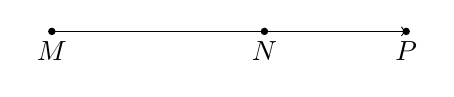
\begin{tikzpicture}[line join = round, line cap = round,scale=.9]
				\coordinate(M) at (0,0);
				\coordinate(N) at (3,0);
				\coordinate(P) at (5,0);
				\draw[->] (M)--(N) (N)--(P);
				\foreach \x in {M,N,P} \fill[black] (\x) circle (1.5pt);
				\path (M) node[below]{$M$};
				\path (N) node[below]{$N$};
				\path (P) node[below]{$P$};
			\end{tikzpicture}

		}
	}
\end{ex}
\begin{ex}%[Sỹ Trường, DỰ ÁN LaTeX hóa Đề cương HK1 - Lớp 10 của Nhóm Tác giả Lê Văn Đoàn]%[0H1Y1-3]
	Gọi $O$ là giao điểm hai đường chéo $AC$ và $BD$ của hình bình hành $ABCD.$ Mệnh đề nào sau đây \textbf{sai}?
	\choice
	{$\overrightarrow{CB}=\overrightarrow{DA}$}
	{$\overrightarrow{OB}=\overrightarrow{DO}$}
	{$\overrightarrow{AB}=\overrightarrow{DC}$}
	{\True $\overrightarrow{OA}=\overrightarrow{OC}$}
	\loigiai{
		\immini
		{
			Ta có $\overrightarrow{OA}=\overrightarrow{CO}$ nên $\overrightarrow{OA}=\overrightarrow{OC}$ là mệnh đề sai.
		}
		{
			\begin{tikzpicture}[line join = round, line cap = round,>=stealth,font=\footnotesize,scale=.6]
				\tkzDefPoints{0/0/D}
				\coordinate (C) at ($(D)+(5,0)$);
				\tkzDefShiftPoint[D](70:3){A}
				\coordinate (B) at ($(A)+(C)-(D)$);
				\coordinate (O) at ($(A)!0.5!(C)$);
				\pgfresetboundingbox
				\tkzDrawPolygon(A,B,C,D)
				\draw (A)--(C) (B)--(D);
				\tkzDrawPoints[fill=black](A,B,C,D,O)
				\tkzLabelPoints[above](A,B)
				\tkzLabelPoints[below](C,D,O)
			\end{tikzpicture}
		}
	}
\end{ex}
\begin{ex}%[Sỹ Trường, DỰ ÁN LaTeX hóa Đề cương HK1 - Lớp 10 của Nhóm Tác giả Lê Văn Đoàn]%[0H1B1-3]
	Cho hình chữ nhật $ABCD$ có $AB=3, AD=4$. Giá trị của $\left|\overrightarrow{AC}\right|$ bằng
	\choice
	{$6$}
	{$3$}
	{$4$}
	{\True $5$}
	\loigiai{
		\immini
		{
			Ta có $\left|\overrightarrow{AC}\right|=AC=\sqrt{AB^2+BC^2}=\sqrt{AB^2+AD^2}=5$.
		}
		{
			\begin{tikzpicture}[line join = round, line cap = round,>=stealth,font=\footnotesize,scale=.6]
				\tkzDefPoints{0/0/D}
				\coordinate (C) at ($(D)+(3,0)$);
				\coordinate (A) at ($(D)+(0,4)$);
				\coordinate (B) at ($(A)+(C)-(D)$);
				\pgfresetboundingbox
				\tkzDrawPolygon(A,B,C,D)
				\draw[->] (A)--(C);
				\tkzDrawPoints[fill=black](A,B,C,D)
				\tkzLabelPoints[above](A,B)
				\tkzLabelPoints[below](C,D)
			\end{tikzpicture}
		}
	}
\end{ex}
\begin{ex}%[Sỹ Trường, DỰ ÁN LaTeX hóa Đề cương HK1 - Lớp 10 của Nhóm Tác giả Lê Văn Đoàn]%[0H1B1-3]
	Cho tam giác $ABC$ vuông tại $A$ có $AB=3, BC=5$. Độ dài của vectơ $\overrightarrow{AC}$ bằng
	\choice
	{$6$}
	{$8$}
	{$13$}
	{\True $4$}
	\loigiai{
		\immini
		{
			Ta có $\left|\overrightarrow{AC}\right|=AC=\sqrt{BC^2-AB^2}=4$.
		}
		{
			\begin{tikzpicture}[line join = round, line cap = round, scale=.6]
				\coordinate[label = left:$A$] (A) at (0,0);
				\coordinate[label = right:$B$] (B) at ($(A)+(3,0)$);
				\coordinate[label = above:$C$] (C) at ($(A)+(0,4)$);
				\draw[fill = gray!50] ($(A)!5pt!(B)$)--($(A)!5pt!(B)+(A)!5pt!(C)-(A)$)--($(A)!5pt!(C)$)--(A)--cycle;
				\draw (A)--(B)--(C)--cycle;
				\foreach \x in {A,B,C} \fill[black] (\x) circle (1.5pt);
			\end{tikzpicture}

		}
	}
\end{ex}
\begin{ex}%[Sỹ Trường, DỰ ÁN LaTeX hóa Đề cương HK1 - Lớp 10 của Nhóm Tác giả Lê Văn Đoàn]%[0H1Y2-5]
	Gọi $M$ là trung điểm của đoạn $AB$. Khẳng định nào sau đây \textbf{sai}?
	\choice
	{\True $\overrightarrow{MA}=\overrightarrow{MB}$}
	{$\overrightarrow{AB}=2 \overrightarrow{MB}$}
	{$\overrightarrow{MA}+\overrightarrow{MB}=\overrightarrow{0}$}
	{$\overrightarrow{MA}=-\dfrac{1}{2} \overrightarrow{AB}$}
	\loigiai{
		\immini
		{
			Ta có $\overrightarrow{MA}=-\overrightarrow{MB}$.
		}
		{
			\begin{tikzpicture}[line join = round, line cap = round,>=stealth,font=\footnotesize,scale=1]
				\tkzDefPoints{0/0/A,4/0/B}
				\coordinate (M) at ($(A)!0.5!(B)$);
				\draw (A)--(B);
				\tkzDrawPoints[fill=black](A,B,M)
				\tkzLabelPoints[below](A,B,M)
			\end{tikzpicture}
		}
	}
\end{ex}
\begin{ex}%[Sỹ Trường, DỰ ÁN LaTeX hóa Đề cương HK1 - Lớp 10 của Nhóm Tác giả Lê Văn Đoàn]%[0H1B3-1]
	Cho tam giác đều $ABC$ với đường cao $AH$. Mệnh đề nào sau đây đúng?
	\choice
	{$\overrightarrow{AB}=\overrightarrow{AC}$}
	{$\left|\overrightarrow{AH}\right|=\dfrac{\sqrt{3}}{2}\left|\overrightarrow{HC}\right|$}
	{$\overrightarrow{HB}=\overrightarrow{HC}$}
	{\True $\left|\overrightarrow{AC}\right|=2\left|\overrightarrow{HC}\right|$}
	\loigiai{
		\immini
		{
			Ta có $2\left|\overrightarrow{HC}\right|=\left|\overrightarrow{BC}\right|=BC=AC=\left|\overrightarrow{AC}\right|$.
		}
		{
			\begin{tikzpicture}[line join = round, line cap = round, scale=1]
				\def \a{2.5};
				\coordinate (B) at (0,0);
				\coordinate (C) at ($(B)+(\a,0)$);
				\coordinate[ shift=(60:\a cm)] (A) at (B);
				\coordinate (H) at ($(B)!0.5!(C)$);
				\draw (A)--(B)--(C)--cycle (A)--(H);
				\foreach \x in {A,B,C,H} \fill[black] (\x) circle (1.2pt);
				\tkzLabelPoints[below](H)
				\tkzLabelPoints[above](A)
				\tkzLabelPoints[left](B)
				\tkzLabelPoints[right](C)
			\end{tikzpicture}

		}
	}
\end{ex}
\begin{ex}%[Sỹ Trường, DỰ ÁN LaTeX hóa Đề cương HK1 - Lớp 10 của Nhóm Tác giả Lê Văn Đoàn]%[0H1Y2-1]
	Cho tam giác $ABC$, trọng tâm $G$. Kết luận nào sau đây đúng?
	\choice
	{Không xác định được $\overrightarrow{GA}+\overrightarrow{GB}+\overrightarrow{GC}$}
	{$\overrightarrow{GA}=\overrightarrow{GB}=\overrightarrow{GC}$}
	{\True $\overrightarrow{GA}+\overrightarrow{GB}+\overrightarrow{GC}=\overrightarrow{0}$}
	{$\overrightarrow{GC}=\overrightarrow{GA}+\overrightarrow{GB}$}
	\loigiai{
		Theo quy tắc trọng tâm của tam giác thì $\overrightarrow{GA}+\overrightarrow{GB}+\overrightarrow{GC}=\overrightarrow{0}$.
	}
\end{ex}
\begin{ex}%[Sỹ Trường, DỰ ÁN LaTeX hóa Đề cương HK1 - Lớp 10 của Nhóm Tác giả Lê Văn Đoàn]%[0H1B1-3]
	Cho tam giác $MNP$ vuông tại $M$ và $MN=3\, \mathrm{cm}, MP=4\, \mathrm{cm}$. Độ dài của $\overrightarrow{NP}$ bằng
	\choice
	{$4\, \mathrm{cm}$}
	{\True $5\, \mathrm{cm}$}
	{$6\, \mathrm{cm}$}
	{$3\, \mathrm{cm}$}
	\loigiai{
		\immini
		{
			Ta có $\left|\overrightarrow{NP}\right|=NP=\sqrt{MN^2+MP^2}=5$.
		}
		{
			\begin{tikzpicture}[line join = round, line cap = round, scale=.6]
				\coordinate[label = left:$M$] (M) at (0,0);
				\coordinate[label = right:$N$] (N) at ($(M)+(3,0)$);
				\coordinate[label = above:$P$] (P) at ($(M)+(0,4)$);
				\draw[fill = gray!50] ($(M)!5pt!(N)$)--($(M)!5pt!(N)+(M)!5pt!(P)-(M)$)--($(M)!5pt!(P)$)--(M)--cycle;
				\draw (M)--(N)--(P)--cycle;
				\foreach \x in {M,N,P} \fill[black] (\x) circle (1.5pt);
			\end{tikzpicture}

		}
	}
\end{ex}
\begin{ex}%[Sỹ Trường, DỰ ÁN LaTeX hóa Đề cương HK1 - Lớp 10 của Nhóm Tác giả Lê Văn Đoàn]%[0H1B1-3]
	Cho hình thoi $ABCD$ tâm $O,$ cạnh bằng $a$ và góc $A$ bằng $60^{\circ}.$ Kết luận nào đúng?
	\choice
	{$|\overrightarrow{OA}|=|\overrightarrow{OB}|$}
	{$|\overrightarrow{OA}|=a$}
	{\True $|\overrightarrow{OA}|=\dfrac{a \sqrt{3}}{2}$}
	{$|\overrightarrow{OA}|=\dfrac{a \sqrt{2}}{2}$}
	\loigiai{
		\immini
		{
			Ta có $\triangle ABD$ là tam giác đều cạnh $a$ nên $|\overrightarrow{OA}|=OA=\dfrac{a \sqrt{3}}{2}$.
		}
		{
			\begin{tikzpicture}[line join = round, line cap = round,>=stealth,font=\footnotesize,scale=0.7]
				\tkzDefPoints{0/0/A}
				\pgfmathsetmacro \gocA{60}; %số đo góc A
				\pgfmathsetmacro \canh{3}; %độ dài cạnh
				\tkzDefShiftPoint[A](\gocA/2:\canh){B}
				\tkzDefShiftPoint[A](-\gocA/2:\canh){D}
				\coordinate (C) at ($(B)+(D)-(A)$);
				\coordinate (O) at ($(A)!0.5!(C)$);
				%
				\pgfresetboundingbox
				\tkzDrawPolygon(A,B,C,D)
				\draw (A)--(C) (B)--(D);
				\tkzDrawPoints[fill=black](A,B,D,C,O)
				\tkzLabelPoints[above](B)
				\tkzLabelPoints[below](D)
				\tkzLabelPoints[left](A)
				\tkzLabelPoints[right](C)
				\tkzLabelPoints[below right](O)

				%			\draw pic[draw,opacity=1.5,angle radius=3mm,angle eccentricity=2,"$60^\circ$"] {angle = D--A--B};

			\end{tikzpicture}
		}
	}
\end{ex}
\begin{ex}%[Sỹ Trường, DỰ ÁN LaTeX hóa Đề cương HK1 - Lớp 10 của Nhóm Tác giả Lê Văn Đoàn]%[0H1Y2-1]
	Cho hình bình hành $ABCD$. Mệnh đề nào sau đây đúng?
	\choice
	{$\overrightarrow{AB}+\overrightarrow{BC}=\overrightarrow{CA}$}
	{$\overrightarrow{BA}+\overrightarrow{AD}=\overrightarrow{AC}$}
	{\True $\overrightarrow{BC}+\overrightarrow{BA}=\overrightarrow{BD}$}
	{$\overrightarrow{AB}+\overrightarrow{AD}=\overrightarrow{CA}$}
	\loigiai{
		Theo quy tắc hình bình hành ta có $\overrightarrow{BC}+\overrightarrow{BA}=\overrightarrow{BD}$.
	}
\end{ex}
\begin{ex}%[Sỹ Trường, DỰ ÁN LaTeX hóa Đề cương HK1 - Lớp 10 của Nhóm Tác giả Lê Văn Đoàn]%[0H1Y1-3]
	Cho hình chữ nhật $ABCD$, gọi $O$ là giao điểm của $AC$ và $BD$. Mệnh đề nào sau đây đúng?
	\choice
	{$\overrightarrow{OA}=\overrightarrow{OB}=\overrightarrow{OC}=\overrightarrow{OD}$}
	{$\overrightarrow{AC}=\overrightarrow{BD}$}
	{$\left|\overrightarrow{OA}+\overrightarrow{OB}+\overrightarrow{OC}+\overrightarrow{OD}\right|=\overrightarrow{0}$}
	{\True $\overrightarrow{AC}-\overrightarrow{AD}=\overrightarrow{AB}$}
	\loigiai{
		\immini
		{
			Ta có $\overrightarrow{AC}-\overrightarrow{AD}=\overrightarrow{DC}=\overrightarrow{AB}$.
		}
		{
			\begin{tikzpicture}[line join = round, line cap = round,>=stealth,font=\footnotesize,scale=.6]
				\tkzDefPoints{0/0/D}
				\coordinate (C) at ($(D)+(5,0)$);
				\coordinate (A) at ($(D)+(0,3)$);
				\coordinate (B) at ($(A)+(C)-(D)$);
				\coordinate (O) at ($(A)!0.5!(C)$);
				\draw (A)--(C) (B)--(D);
				\pgfresetboundingbox
				\tkzDrawPolygon(A,B,C,D)
				\tkzDrawPoints[fill=black](A,B,C,D,O)
				\tkzLabelPoints[above](A,B)
				\tkzLabelPoints[below](C,D,O)
			\end{tikzpicture}
		}
	}
\end{ex}
\begin{ex}%[Sỹ Trường, DỰ ÁN LaTeX hóa Đề cương HK1 - Lớp 10 của Nhóm Tác giả Lê Văn Đoàn]%[0H1B2-5]
	Cho tam giác $ABC$ vuông tại $A$ có $AB=3, BC=5$. Tính $\left|\overrightarrow{AB}+\overrightarrow{BC}\right|$.
	\choice
	{\True $4$}
	{$5$}
	{$6$}
	{$3$}
	\loigiai{
		\immini
		{
			Ta có $\left|\overrightarrow{AB}+\overrightarrow{BC}\right|=\left|\overrightarrow{AC}\right|=AC=\sqrt{BC^2-AB^2}=4$.
		}
		{
			\begin{tikzpicture}[line join = round, line cap = round, scale=.6]
				\coordinate[label = left:$A$] (A) at (0,0);
				\coordinate[label = right:$B$] (B) at ($(A)+(3,0)$);
				\coordinate[label = above:$C$] (C) at ($(A)+(0,4)$);
				\draw[fill = gray!50] ($(A)!5pt!(B)$)--($(A)!5pt!(B)+(A)!5pt!(C)-(A)$)--($(A)!5pt!(C)$)--(A)--cycle;
				\draw (A)--(B)--(C)--cycle;
				\foreach \x in {A,B,C} \fill[black] (\x) circle (1.5pt);
			\end{tikzpicture}

		}
	}
\end{ex}
\begin{ex}%[Sỹ Trường, DỰ ÁN LaTeX hóa Đề cương HK1 - Lớp 10 của Nhóm Tác giả Lê Văn Đoàn]%[0H1Y2-1]
	Cho bốn điểm bất kỳ $A,B,C,O$. Mệnh đề nào sau đây là đúng?
	\choice
	{$\overrightarrow{OA}=\overrightarrow{OB}-\overrightarrow{BA}$}
	{$\overrightarrow{OA}=\overrightarrow{CA}+\overrightarrow{CO}$}
	{\True $\overrightarrow{BC}-\overrightarrow{AC}+\overrightarrow{AB}=\overrightarrow{0}$}
	{$\overrightarrow{BA}=\overrightarrow{OB}-\overrightarrow{OA}$}
	\loigiai{
		Ta có $\overrightarrow{BC}-\overrightarrow{AC}+\overrightarrow{AB}=\overrightarrow{AB}+\overrightarrow{BC}-\overrightarrow{AC}=\overrightarrow{AC}-\overrightarrow{AC}=\overrightarrow{0}$.
	}
\end{ex}
\begin{ex}%[Sỹ Trường, DỰ ÁN LaTeX hóa Đề cương HK1 - Lớp 10 của Nhóm Tác giả Lê Văn Đoàn]%[0H1Y2-1]
	Điều kiện cần và đủ để điểm $O$ là trung điểm của đoạn $AB$ là
	\choice
	{$OA=OB$}
	{$\overrightarrow{OA}=\overrightarrow{OB}$}
	{$\overrightarrow{AO}=\overrightarrow{BO}$}
	{\True $\overrightarrow{OA}+\overrightarrow{OB}=\overrightarrow{0}$}
	\loigiai{
		Điểm $O$ là trung điểm của đoạn $AB$ khi và chỉ khi $\overrightarrow{OA}+\overrightarrow{OB}=\overrightarrow{0}$.
	}
\end{ex}
\begin{ex}%[Sỹ Trường, DỰ ÁN LaTeX hóa Đề cương HK1 - Lớp 10 của Nhóm Tác giả Lê Văn Đoàn]%[0H1Y2-5]
	Cho tam giác $ABC$ đều có độ dài cạnh bằng $a$. Khi đó $\left|\overrightarrow{AB}+\overrightarrow{BC}\right|$ bằng
	\choice
	{$\dfrac{a \sqrt{3}}{2}$}
	{\True $a$}
	{$2a$}
	{$a \sqrt{3}$}
	\loigiai{
		Ta có $\left|\overrightarrow{AB}+\overrightarrow{BC}\right|=\left|\overrightarrow{AC}\right|=a$.
	}
\end{ex}
\begin{ex}%[Sỹ Trường, DỰ ÁN LaTeX hóa Đề cương HK1 - Lớp 10 của Nhóm Tác giả Lê Văn Đoàn]%[0H1B2-5]
	Cho tam giác $ABC$ vuông tại $A$ và $AB=3, AC=4$. Vectơ $\overrightarrow{CB}+\overrightarrow{AB}$ có độ dài bằng
	\choice
	{\True $2 \sqrt{13}$}
	{$2 \sqrt{3}$}
	{$\sqrt{3}$}
	{$\sqrt{13}$}
	\loigiai{
		\immini
		{
			Kẻ $\overrightarrow{BD}=\overrightarrow{AB}$, khi đó ta có $\overrightarrow{CB}+\overrightarrow{AB}=\overrightarrow{CB}+\overrightarrow{BD}=\overrightarrow{CD}$.\\
			Xét $\triangle ADC$ vuông tại $A$ có $CD=\sqrt{AD^2+AC^2}=\sqrt{6^2+4^2}=2\sqrt{13}.$\\
			Vậy $\left|\overrightarrow{CB}+\overrightarrow{AB}\right|=2\sqrt{13}$.
		}
		{
			\begin{tikzpicture}[line join = round, line cap = round, scale=.6]
				\coordinate[label = left:$A$] (A) at (0,0);
				\coordinate[label = below:$B$] (B) at ($(A)+(3,0)$);
				\coordinate[label = above:$C$] (C) at ($(A)+(0,4)$);
				\coordinate[label = right:$D$] (D) at ($(B)+(B)-(A)$);

				\draw[fill = gray!50] ($(A)!5pt!(B)$)--($(A)!5pt!(B)+(A)!5pt!(C)-(A)$)--($(A)!5pt!(C)$)--(A)--cycle;
				\draw (A)--(B)--(C)--cycle (B)--(D)--(C);
				\foreach \x in {A,B,C,D} \fill[black] (\x) circle (1.5pt);
			\end{tikzpicture}

		}
	}
\end{ex}
\begin{ex}%[Sỹ Trường, DỰ ÁN LaTeX hóa Đề cương HK1 - Lớp 10 của Nhóm Tác giả Lê Văn Đoàn]%[0H1Y2-5]
	Cho tam giác $ABC$ đều có độ dài cạnh bằng $2a$. Độ dài của $\overrightarrow{AB}+\overrightarrow{BC}$ bằng
	\choice
	{$a \sqrt{3}$}
	{\True $2a$}
	{$2a \sqrt{3}$}
	{$\dfrac{a \sqrt{3}}{2}$}
	\loigiai{
		Ta có $\overrightarrow{AB}+\overrightarrow{BC}=\overrightarrow{AC}$.\\
		Do đó $\left|\overrightarrow{AB}+\overrightarrow{BC}\right|=AC=2a$.
	}
\end{ex}
%10
\begin{ex}%Câu 21%[Huỳnh Đức Vũ, Dự án Tex hóa đề cương HK1-Lớp 10-Nhóm tác giả Lê Văn Đoàn]%[0H1Y2-1]
	Cho tam giác $ABC$. Gọi $M$, $N$, $P$ lần lượt là trung điểm các cạnh $AB$, $AC$, $BC$. Hỏi $\overrightarrow{MP}+\overrightarrow{NP}$ bằng vectơ nào?
	\choice
	{$\overrightarrow{PB}$}
	{\True $\overrightarrow{AP}$}
	{$\overrightarrow{MN}$}
	{$\overrightarrow{AM}$}
	\loigiai{
		\immini{
			Ta có $\overrightarrow{MP}+\overrightarrow{NP}=\overrightarrow{AN}+\overrightarrow{NP}=\overrightarrow{AP}$.
		}{
			\begin{tikzpicture}[scale=1, font=\footnotesize, line join=round, line cap=round, >=stealth]
				\path
				(0,2) coordinate(A)
				(2,0) coordinate(B)
				(-1,0) coordinate(C)
				($(A)!0.5!(B)$) coordinate(M)
				($(A)!0.5!(C)$) coordinate(N)
				($(C)!0.5!(B)$) coordinate(P)
				;
				\draw (A)--(B)--(C)--(A) (M)--(N)--(P)--(M);
				\foreach \x/\g in {A/90,B/-90,C/-90,M/45,N/135,P/-90}
				\fill[black] (\x) circle(1pt) ($(\x)+(\g:3mm)$) node{$\x$};
			\end{tikzpicture}
		}
	}
\end{ex}

\begin{ex}%Câu 22%[Huỳnh Đức Vũ, Dự án Tex hóa đề cương HK1-Lớp 10-Nhóm tác giả Lê Văn Đoàn]%[0H1Y2-1]
	Cho hình bình hành $ABCD$, giao điểm của hai đường chéo là $ O$. Tìm mệnh đề \textbf{sai}?
	\choice
	{$\overrightarrow{DA}-\overrightarrow{DB}=\overrightarrow{OD}-\overrightarrow{OC}$}
	{\True $\overrightarrow{DA}+\overrightarrow{DB}+\overrightarrow{DC}=\overrightarrow{0}$}
	{$\overrightarrow{CO}-\overrightarrow{OB}=\overrightarrow{BA}$}
	{$\overrightarrow{AB}-\overrightarrow{BC}=\overrightarrow{DB}$}
	\loigiai{\immini{
			Theo quy tắc hình bình hành, ta có $\overrightarrow{DA}+\overrightarrow{DC}=\overrightarrow{DB}$.\\
			Do đó $\overrightarrow{DA}+\overrightarrow{DB}+\overrightarrow{DC}=\overrightarrow{DB}+\overrightarrow{DB}=2\overrightarrow{DB}\ne \overrightarrow{0}$.\\
			Vậy mệnh đề: \lq \lq $\overrightarrow{DA}+\overrightarrow{DB}+\overrightarrow{DC}=\overrightarrow{0}$ \rq \rq \; là mệnh đề sai và dễ dàng kiểm tra được các mệnh đề còn lại là các mệnh đề đúng.

		}{\begin{tikzpicture}[scale=1, font=\footnotesize, line join=round, line cap=round, >=stealth]
				\path
				(3,2) coordinate(A)
				(2,0) coordinate(B)
				(-1,0) coordinate(C)
				($(A)!0.5!(C)$) coordinate(O);
				\coordinate (D) at ($(A)+(C)-(B)$);
				\draw (A)--(B)--(C)--(D)--(A)--(C)
				(B)--(D);
				\foreach \x/\g in {A/90,B/-90,C/-90,O/-90, D/90}
				\fill[black] (\x) circle(1pt) ($(\x)+(\g:3mm)$) node{$\x$};
	\end{tikzpicture}}}
\end{ex}

\begin{ex}%Câu 23%[Huỳnh Đức Vũ, Dự án Tex hóa đề cương HK1-Lớp 10-Nhóm tác giả Lê Văn Đoàn]%%[0H1B2-5]
	Cho tam giác $ABC$, trọng tâm $ G$. Phát biểu nào đúng?
	\choice
	{$\overrightarrow{AB}+\overrightarrow{BC}=\left|\overrightarrow{AC}\right|$}
	{$\left|\overrightarrow{GA}\right|+\left|\overrightarrow{GB}\right|+\left|\overrightarrow{GC}\right|=0$}
	{$\left|\overrightarrow{AB}+\overrightarrow{BC}\right|=\overrightarrow{AC}$}
	{\True $\left|\overrightarrow{GA}+\overrightarrow{GB}+\overrightarrow{GC}\right|=0$}
	\loigiai{\immini{
			Theo tính chất trọng tâm tam giác, ta có $$\overrightarrow{GA}+\overrightarrow{GB}+\overrightarrow{GC}=\overrightarrow{0}.$$
			Vậy  $\left|\overrightarrow{GA}+\overrightarrow{GB}+\overrightarrow{GC}\right|=0$.
		}{\begin{tikzpicture}[scale=1, font=\footnotesize, line join=round, line cap=round, >=stealth]
				\pgfmathsetmacro{\k}{2/3};
				\path
				(0,2) coordinate(A)
				(2,0) coordinate(B)
				(-1,0) coordinate(C)
				($(C)!0.5!(B)$) coordinate(M)
				($(A)!\k!(M)$) coordinate(G)
				;
				\draw (A)--(B)--(C)--(A)--(M) ;
				\foreach \x/\g in {A/90,B/-90,C/-90,M/-90, G/0}
				\fill[black] (\x) circle(1pt) ($(\x)+(\g:3mm)$) node{$\x$};
	\end{tikzpicture}}}
\end{ex}

\begin{ex}%Câu 24%[Huỳnh Đức Vũ, Dự án Tex hóa đề cương HK1-Lớp 10-Nhóm tác giả Lê Văn Đoàn]%[0H1Y2-1]
	Cho lục giác đều $ABCDEF$ và $ O$ là tâm của nó. Đẳng thức nào\textbf{ sai}?
	\choice
	{$\overrightarrow{OA}+\overrightarrow{OC}+\overrightarrow{OE}=\overrightarrow{0}$}
	{$\overrightarrow{BC}+\overrightarrow{FE}=\overrightarrow{AD}$}
	{$\overrightarrow{OA}+\overrightarrow{OB}+\overrightarrow{OC}=\overrightarrow{EB}$ }
	{\True $\overrightarrow{AB}+\overrightarrow{CD}+\overrightarrow{FE}=\overrightarrow{0}$}
	\loigiai{
		\immini{
			Ta có $$\overrightarrow{AB}+\overrightarrow{CD}+\overrightarrow{FE}=\overrightarrow{0}=\overrightarrow{AB}+\overrightarrow{BO}+\overrightarrow{OA}=\overrightarrow{0}.$$
		}{
			\begin{tikzpicture}[scale=0.8, font=\footnotesize, line join=round, line cap=round, >=stealth]
				\path
				(0:0) coordinate (O)
				(0:1.5) coordinate (A)
				(60:1.5) coordinate (B)
				(120:1.5) coordinate (C)
				(180:1.5) coordinate (D)
				(-120:1.5) coordinate (E)
				(-60:1.5) coordinate (F)
				;
				\draw (A)--(B)--(C)--(D)--(E)--(F)--(A)--(D) (B)--(E) (C)--(F);
				\foreach \x/\g in {A/0,B/60,C/120,D/180,E/-120,F/-60,O/90}
				\fill[black] (\x) circle(1pt) ($(\x)+(\g:3mm)$) node{$\x$};
			\end{tikzpicture}
		}
	}
\end{ex}

\begin{ex}%Câu 25%[Huỳnh Đức Vũ, Dự án Tex hóa đề cương HK1-Lớp 10-Nhóm tác giả Lê Văn Đoàn]%[0H1Y2-1]
	Cho bốn điểm $A$, $B$, $ C$, $ D$ phân biệt. Khi đó $\overrightarrow{AB}-\overrightarrow{DC}+\overrightarrow{BC}-\overrightarrow{AD}$ bằng
	\choice
	{$\overrightarrow{AC}$}
	{$ 2\overrightarrow{DC}$}
	{\True $\overrightarrow{0}$}
	{$\overrightarrow{BD}$}
	\loigiai{
		Ta có $\overrightarrow{AB}-\overrightarrow{DC}+\overrightarrow{BC}-\overrightarrow{AD}=\overrightarrow{AB}+\overrightarrow{BC}+\overrightarrow{CD}+\overrightarrow{DA}=\overrightarrow{AC}+\overrightarrow{CA}=\overrightarrow{0}$.
	}
\end{ex}

\begin{ex}%Câu 26%[Huỳnh Đức Vũ, Dự án Tex hóa đề cương HK1-Lớp 10-Nhóm tác giả Lê Văn Đoàn]%[0H1Y2-1]
	Cho ba điểm $A$, $B$, $ C$ phân biệt. Đẳng thức nào sau đây \textbf{sai}?
	\choice
	{$\overrightarrow{AB}+\overrightarrow{BC}=\overrightarrow{AC}$}
	{\True $\overrightarrow{CA}+\overrightarrow{AB}=\overrightarrow{BC}$}
	{$\overrightarrow{BA}+\overrightarrow{AC}=\overrightarrow{BC}$}
	{$\overrightarrow{AB}-\overrightarrow{AC}=\overrightarrow{CB}$}
	\loigiai{
		Ta có $\overrightarrow{CA}+\overrightarrow{AB}=\overrightarrow{CB}\ne \overrightarrow{BC}$.
	}
\end{ex}

\begin{ex}%Câu 27%[Huỳnh Đức Vũ, Dự án Tex hóa đề cương HK1-Lớp 10-Nhóm tác giả Lê Văn Đoàn]%[0H1Y2-5]
	Cho hình vuông $ABCD$ có cạnh bằng $a$. Khi đó $\left|\overrightarrow{AB}+\overrightarrow{AD}\right|$ bằng
	\choice
	{\True $a\sqrt{2}$}
	{$\dfrac{a\sqrt{2}}{2}$}
	{$ 2a$}
	{$a$}
	\loigiai{ \immini{
			Áp dụng tính chất hình bình hành ta có $\overrightarrow{AB}+\overrightarrow{AD}=\overrightarrow{AC}$.\\
			Do đó $\left|\overrightarrow{AB}+\overrightarrow{AD}\right|=\left|\overrightarrow{AC}\right|=a\sqrt{2}$.
		}{\begin{tikzpicture}[scale=1, font=\footnotesize, line join=round, line cap=round, >=stealth]
				\def\a{2.5}
				\path
				(0:0) coordinate (A)
				(0:\a) coordinate (B)
				(-90:\a) coordinate (D)
				($(B)+(-90:\a)$) coordinate (C)
				;
				\draw (A)--(D)--(C)--(B)--(A)
				(A)--(C);
				\foreach \x/\g in {A/90,B/90,C/-90,D/-90}
				\fill[black] (\x) circle(1pt) ($(\x)+(\g:3mm)$) node{$\x$};
				\foreach \x/\o/\y/\r in {A/D/C/2} \draw ($(\o)!\r mm!(\x)$)--($($(\o)!\r mm!(\x)$)+($(\o)!\r mm!(\y)$)-(\o)$)--($(\o)!\r mm!(\y)$);
				\draw (A)--(D)--(C);
	\end{tikzpicture}}}
\end{ex}

\begin{ex}%Câu 28%[Huỳnh Đức Vũ, Dự án Tex hóa đề cương HK1-Lớp 10-Nhóm tác giả Lê Văn Đoàn]%[0H1Y2-5]
	Cho hình vuông $ABCD$ có cạnh bằng $a$. Khi đó $\left|\overrightarrow{AB}+\overrightarrow{AC}\right|$ bằng
	\choice
	{\True $a\sqrt{5}$}
	{$a\sqrt{3}$}
	{$\dfrac{a\sqrt{3}}{3}$}
	{$\dfrac{a\sqrt{5}}{2}$}
	\loigiai{
		\immini{Gọi $E$ là đỉnh thứ tư của hình bình hành $ABEC$ và $F$ là hình chiếu của $E$ lên đường thẳng $AB$.\\
			Khi đó $\left|\overrightarrow{AB}+\overrightarrow{BC}\right|=\left|\overrightarrow{AE}\right|$.\\
			Xét tam giác $AEF$ vuông tại $F$, có $AF=2a$, $EF=a$, do đó $$AE=\sqrt{AF^2+EF^2}=\sqrt{4a^2+a^2}=a\sqrt{5}.$$}{
			\begin{tikzpicture}[scale=1, font=\footnotesize, line join=round, line cap=round, >=stealth]
				\def\r{1.5}
				\path
				(0:0) coordinate (A)
				(0:\r) coordinate (B)
				(-90:\r) coordinate (D)
				($(B)+(-90:\r)$) coordinate (C)
				(0:2*\r) coordinate (F)
				($(C)+(0:\r)$) coordinate (E)
				;
				\draw (A)--(D)--(C)--(B)--(A)--(E)--(F)--(B)(A)--(C)
				(B)--(E)
				(C)--(E);
				\foreach \x/\g in {A/90,B/90,C/-90,D/-90,E/-90,F/90}
				\fill[black] (\x) circle(1pt) ($(\x)+(\g:3mm)$) node{$\x$};
				\foreach \x/\o/\y/\r in {A/D/C/2} \draw ($(\o)!\r mm!(\x)$)--($($(\o)!\r mm!(\x)$)+($(\o)!\r mm!(\y)$)-(\o)$)--($(\o)!\r mm!(\y)$);
				\draw (A)--(D)--(C);
			\end{tikzpicture}
		}
	}
\end{ex}

\begin{ex}%Câu 29%[Huỳnh Đức Vũ, Dự án Tex hóa đề cương HK1-Lớp 10-Nhóm tác giả Lê Văn Đoàn]%[0H1Y2-5]
	Cho hình chữ nhật $ABCD$, biết $AB=4a$ và $AD=3a$. Tính độ dài của vectơ $\overrightarrow{AB}+\overrightarrow{AD}$.
	\choice
	{\True $ 5a$}
	{$ 6a$}
	{$ 2a\sqrt{3}$}
	{$ 7a$}
	\loigiai{
		\immini{
			Theo tính chất hình bình hành, ta có $$\left|\overrightarrow{AB}+\overrightarrow{AD}\right|=\left|\overrightarrow{AC}\right|=\sqrt{AB^2+AD^2}=\sqrt{16a^2+9a^2}=5a.$$}
		{\begin{tikzpicture}[scale=0.8, font=\footnotesize, line join=round, line cap=round, >=stealth]
				\def\a{0.8}
				\path
				(0:0) coordinate (A)
				(0:4*\a) coordinate (B)
				(-90:3*\a) coordinate (D)
				($(B)+(-90:3*\a)$) coordinate (C)
				;
				\draw (A)--(D)--(C)--(B)--(A)
				(A)--(C);
				\foreach \x/\g in {A/90,B/90,C/-90,D/-90}
				\fill[black] (\x) circle(1pt) ($(\x)+(\g:3mm)$) node{$\x$};
				\foreach \x/\o/\y/\r in {A/D/C/2} \draw ($(\o)!\r mm!(\x)$)--($($(\o)!\r mm!(\x)$)+($(\o)!\r mm!(\y)$)-(\o)$)--($(\o)!\r mm!(\y)$);
				\draw (A)--(D)--(C);
		\end{tikzpicture}}
	}
\end{ex}
\begin{ex}%Câu 30%[Huỳnh Đức Vũ, Dự án Tex hóa đề cương HK1-Lớp 10-Nhóm tác giả Lê Văn Đoàn]%[0H1Y3-1]
	Cho hình vuông $ABCD$ cạnh $a$. Giá trị của $\left|\overrightarrow{AB}+\overrightarrow{AC}+\overrightarrow{AD}\right|$ bằng
	\choice
	{$A\sqrt{2}$}
	{$ 2a$}
	{\True $ 2a\sqrt{2}$}
	{$ 3a$}
	\loigiai{\immini{
			Ta có $$\left|\overrightarrow{AB}+\overrightarrow{AC}+\overrightarrow{AD}\right|=\left|\overrightarrow{AC}+\overrightarrow{AC}\right|=2\left|\overrightarrow{AC}\right|=2AC=2a\sqrt{2}.$$}
		{\begin{tikzpicture}[scale=1, font=\footnotesize, line join=round, line cap=round, >=stealth]
				\def\a{2.5}
				\path
				(0:0) coordinate (A)
				(0:\a) coordinate (B)
				(-90:\a) coordinate (D)
				($(B)+(-90:\a)$) coordinate (C)
				;
				\draw (A)--(D)--(C)--(B)--(A)
				(A)--(C);
				\foreach \x/\g in {A/90,B/90,C/-90,D/-90}
				\fill[black] (\x) circle(1pt) ($(\x)+(\g:3mm)$) node{$\x$};
				\foreach \x/\o/\y/\r in {A/D/C/2} \draw ($(\o)!\r mm!(\x)$)--($($(\o)!\r mm!(\x)$)+($(\o)!\r mm!(\y)$)-(\o)$)--($(\o)!\r mm!(\y)$);
				\draw (A)--(D)--(C);
		\end{tikzpicture}}
	}
\end{ex}

\begin{ex}%Câu 31%[Huỳnh Đức Vũ, Dự án Tex hóa đề cương HK1-Lớp 10-Nhóm tác giả Lê Văn Đoàn]%[0H1Y3-1]
	Cho tam giác đều $ABC$ cạnh $ 4a$. Độ dài $\overrightarrow{AB}+\overrightarrow{AC}$ là
	\choice
	{$ 2a\sqrt{3}$}
	{$a\sqrt{5}$}
	{$a\sqrt{6}$}
	{\True $ 4a\sqrt{3}$}
	\loigiai{\immini{
			Gọi $M$ là trung điểm của $BC$ .\\
			Vì $AM$ là đường trung tuyến của tam giác đều cạnh $4a$ nên $$AM=\dfrac{4a\sqrt{3}}{2}=2a\sqrt{3}.$$
			Do đó $\left|\overrightarrow{AB}+\overrightarrow{AC}\right|=\left|2\overrightarrow{AM}\right|=2AM=4a\sqrt{3}$.
		}
		{	\begin{tikzpicture}[scale=0.8,>=stealth, font=\footnotesize, line join=round, line cap=round]
				\def\xmin{-4} \def\xmax{5}  \def\ymin{-0.3}  \def\ymax{4}
				\clip (\xmin,\ymin) rectangle (\xmax,\ymax);
				\def\a{3.5}
				\pgfmathsetmacro{\y}{\a*(sqrt(3)/2)};
				\coordinate (A) at (0,0);
				\coordinate (B) at (\a,0);
				\coordinate (C) at (\a/2,\y);
				\coordinate (M) at ($(C)!0.5!(B)$);
				\filldraw (A) circle(1pt) node[left]{$A$};
				\filldraw (B) circle(1pt) node[right]{$B$};
				\filldraw (C) circle(1pt) node[above]{$C$};
				\filldraw (M) circle(1pt) node[right]{$M$};
				\draw(A)--(B)--(C)--cycle
				(A)--(M);
				\foreach \x/\o/\y/\r in {A/M/B/2} \draw ($(\o)!\r mm!(\x)$)--($($(\o)!\r mm!(\x)$)+($(\o)!\r mm!(\y)$)-(\o)$)--($(\o)!\r mm!(\y)$);
				\draw (A)--(M)--(B);
	\end{tikzpicture}}}
\end{ex}

\begin{ex}%Câu 32[Huỳnh Đức Vũ, Dự án Tex hóa đề cương HK1-Lớp 10-Nhóm tác giả Lê Văn Đoàn]%[0H1B3-1]
	Cho ba lực $\overrightarrow{F_1}=\overrightarrow{MA}$, $\overrightarrow{F_2}=\overrightarrow{MB}$, $\overrightarrow{F_3}=\overrightarrow{MC}$ cùng tác động vào một vật tại điểm $M$ và vật đứng yên.
	\immini{Cho biết cường độ của $\overrightarrow{F_1}$, $\overrightarrow{F_2}$ đều bằng $ 100\,N$ và $\widehat{AMB}=60^\circ $. Khi đó cường độ lực của $\overrightarrow{F_3}$ bằng
		\choice
		{$ 50\sqrt{2}\,N$}
		{$ 50\sqrt{3}\,N$}
		{$ 25\sqrt{3}\,N$}
		{\True $ 100\sqrt{3}\,N$} }{
		\begin{tikzpicture}[scale=0.6, font=\footnotesize, line join=round, line cap=round, >=stealth]
			\path
			(0:0) coordinate (M)
			(30:2) coordinate (A)
			(-30:2) coordinate (B)
			(180:4) coordinate (C)
			($(M)!0.5!(A)$) coordinate (d)
			($(M)!0.5!(B)$) coordinate (e)
			($(M)!0.5!(C)$) coordinate (f)
			;
			\draw[->] (M)--(A);
			\draw[->] (M)--(B);
			\draw[->] (M)--(C);
			\fill[black] (M) circle(1pt) node[above]{$M$};
			\draw
			(A) node[above right]{$A$}
			(B) node[below right]{$B$}
			(C) node[left]{$C$}
			(d) node[above left]{$\overrightarrow{F_1}$}
			(e) node[below left]{$\overrightarrow{F_2}$}
			(f) node[above]{$\overrightarrow{F_3}$}
			;
		\end{tikzpicture}
	}
	\loigiai{\immini{
			Gọi $D$ là đỉnh thứ tư của hình bình hành $MADB$.\\ Khi đó hợp lực  $\overrightarrow{F_1}+\overrightarrow{F_2}=\overrightarrow{MA}+\overrightarrow{MB}=\overrightarrow{MD}$.\\
			$MD=2MO=2\cdot\dfrac{100\sqrt{3}}{2}=100\sqrt{3}$.\\
			Vậy hợp lực $\overrightarrow{F_1}+\overrightarrow{F_2}$ có độ lớn $100\sqrt{3}$.\\
			Vì điểm $M$ đứng yên nên độ lớn của lực $\overrightarrow{F_3}$ là $100\sqrt{3} N$.
		}
		{\begin{tikzpicture}[scale=0.8, font=\footnotesize, line join=round, line cap=round, >=stealth]
				\path
				(0:0) coordinate (M)
				(30:3) coordinate (A)
				(-30:3) coordinate (B)
				(180:3) coordinate (C)
				($(M)!0.5!(A)$) coordinate (d)
				($(M)!0.5!(B)$) coordinate (e)
				($(M)!0.5!(C)$) coordinate (f)
				($(A)!0.5!(B)$) coordinate (O);
				\coordinate (D) at ($(A)+(B)-(M)$);
				\draw[->] (M)--(A);
				\draw[->] (M)--(B);
				\draw[->] (M)--(C);
				\draw[->] (A)--(D);
				\draw[->] (B)--(D);
				\draw[->] (C)--(D);
				\draw (A)--(B);
				\fill[black] (M) circle(1pt) node[above]{$M$};
				\fill[black] (O) circle(1pt) node[below left]{$O$};
				\fill[black] (A) circle(1pt) node[above]{$A$};
				\fill[black] (B) circle(1pt) node[below]{$B$};
				\draw
				(C) node[left]{$C$}
				(D) node[right]{$D$}
				(d) node[above left]{$\overrightarrow{F_1}$}
				(e) node[below left]{$\overrightarrow{F_2}$}
				(f) node[above]{$\overrightarrow{F_3}$}
				;
				\foreach \x/\o/\y/\r in {D/O/A/2} \draw ($(\o)!\r mm!(\x)$)--($($(\o)!\r mm!(\x)$)+($(\o)!\r mm!(\y)$)-(\o)$)--($(\o)!\r mm!(\y)$);
				\draw (D)--(O)--(A);
				\draw[-] ($(M)!4mm!(B)$) to[bend right=45] node[pos=.1,right]{$60^\circ$} ($(M)!4mm!(A)$);
	\end{tikzpicture}}}

\end{ex}

\begin{ex}%Câu 33[Huỳnh Đức Vũ, Dự án Tex hóa đề cương HK1-Lớp 10-Nhóm tác giả Lê Văn Đoàn]%[0H1Y3-1]
	Cho hình thoi $ABCD$ cạnh $a$, tâm $O$ và $\widehat{BAD}=60^\circ$. Độ dài vectơ $\overrightarrow{OB}-\overrightarrow{CD}$ bằng
	\choice
	{\True $\dfrac{a\sqrt{7}}{2}$}
	{$\dfrac{a\sqrt{5}}{2}$}
	{$2a$}
	{$a\sqrt{3}$}
	\loigiai{
		\immini{
			Gọi $G$ là trung điểm của đoạn $OC$.\\
			Ta có $\left|\overrightarrow{OB}-\overrightarrow{CD}\right|=\left|\overrightarrow{DO}+\overrightarrow{DC}\right|=2\left|\overrightarrow{DG}\right|=2DG$.\\
			Tam giác $DOG$ vuông tại $O$ có $DO=\dfrac{a}{2}$, $OG=\dfrac{OC}{2}=\dfrac{a\sqrt{3}}{4}$ nên $$2DG=\sqrt{DO^2+OG^2}=2\sqrt{\left(\dfrac{a}{2}\right)^2+\left(\dfrac{a\sqrt{3}}{4}\right)^2}=\dfrac{a\sqrt{7}}{2}.$$
		}{
			\begin{tikzpicture}[scale=1, font=\footnotesize, line join=round, line cap=round, >=stealth]
				\def\r{2}
				\path
				(0:0) coordinate (B)
				(30:\r) coordinate (C)
				(90:\r) coordinate (D)
				(150:\r) coordinate (A)
				($(A)!0.5!(C)$) coordinate (O)
				($(O)!0.5!(C)$) coordinate (G)
				;
				\draw (A)--(B)--(C)--(D)--(A)--(C) (B)--(D)--(G);
				\foreach \x/\g in {A/-90,B/-90,C/-90,D/90,O/-45, G/-90}
				\fill[black] (\x) circle(1pt) ($(\x)+(\g:3mm)$) node{$\x$};
				\foreach \x/\o/\y/\r in {D/O/A/2} \draw ($(\o)!\r mm!(\x)$)--($($(\o)!\r mm!(\x)$)+($(\o)!\r mm!(\y)$)-(\o)$)--($(\o)!\r mm!(\y)$);
				\draw (D)--(O)--(A);
				\draw[-] ($(A)!4mm!(B)$) to[bend right=45] node[pos=.1,right]{$60^\circ$} ($(A)!4mm!(D)$);
			\end{tikzpicture}
		}
	}
\end{ex}


\begin{ex}%Câu 34%[Huỳnh Đức Vũ, Dự án Tex hóa đề cương HK1-Lớp 10-Nhóm tác giả Lê Văn Đoàn]%[0H1Y2-5]
	Cho hình vuông $ABCD$ cạnh $a$. Giá trị $\left|\overrightarrow{AB}-\overrightarrow{DA}\right|$ bằng
	\choice
	{\True $A\sqrt{2}$}
	{$ 2a$}
	{$ 0$}
	{$A$}
	\loigiai{ \immini{
			Ta có $$\left|\overrightarrow{AB}-\overrightarrow{DA}\right|=\left|\overrightarrow{AB}+\overrightarrow{AD}\right|=\left|\overrightarrow{AC}\right|=AC=a\sqrt{2}.$$
		}
		{\begin{tikzpicture}[scale=1, font=\footnotesize, line join=round, line cap=round, >=stealth]
				\def\a{2.5}
				\path
				(0:0) coordinate (A)
				(0:\a) coordinate (B)
				(-90:\a) coordinate (D)
				($(B)+(-90:\a)$) coordinate (C)
				;
				\draw (A)--(D)--(C)--(B)--(A)
				(A)--(C);
				\foreach \x/\g in {A/90,B/90,C/-90,D/-90}
				\fill[black] (\x) circle(1pt) ($(\x)+(\g:3mm)$) node{$\x$};
				\foreach \x/\o/\y/\r in {A/D/C/2} \draw ($(\o)!\r mm!(\x)$)--($($(\o)!\r mm!(\x)$)+($(\o)!\r mm!(\y)$)-(\o)$)--($(\o)!\r mm!(\y)$);
				\draw (A)--(D)--(C);
	\end{tikzpicture}}}
\end{ex}

\begin{ex}%Câu 35%[Huỳnh Đức Vũ, Dự án Tex hóa đề cương HK1-Lớp 10-Nhóm tác giả Lê Văn Đoàn]%[0H1Y2-5]
	Cho hình vuông $ABCD$ cạnh $a$, tâm $O$. Giá trị của $\left|\overrightarrow{OB}+\overrightarrow{OC}\right|$ bằng
	\choice
	{$a\sqrt{2}$}
	{\True $a$}
	{$\dfrac{a}{2}$}
	{$\dfrac{a\sqrt{2}}{2}$}
	\loigiai{ \immini{
			Ta có $$\left|\overrightarrow{OB}+\overrightarrow{OC}\right|=\left|\overrightarrow{DO}+\overrightarrow{OC}\right|=\left|\overrightarrow{DC}\right|=DC=a.$$}
		{\begin{tikzpicture}[scale=1, font=\footnotesize, line join=round, line cap=round, >=stealth]
				\def\a{2.5}
				\path
				(0:0) coordinate (A)
				(0:\a) coordinate (B)
				(-90:\a) coordinate (D)
				($(B)+(-90:\a)$) coordinate (C);
				\coordinate (O) at ($(A)!0.5!(C)$)
				;
				\draw (A)--(D)--(C)--(B)--(A)
				(A)--(C)
				(B)--(D);
				\foreach \x/\g in {A/90,B/90,C/-90,D/-90, O/-90}
				\fill[black] (\x) circle(1pt) ($(\x)+(\g:3mm)$) node{$\x$};
				\foreach \x/\o/\y/\r in {A/D/C/2} \draw ($(\o)!\r mm!(\x)$)--($($(\o)!\r mm!(\x)$)+($(\o)!\r mm!(\y)$)-(\o)$)--($(\o)!\r mm!(\y)$);
	\end{tikzpicture}}}
\end{ex}

\begin{ex}%Câu 36%[Huỳnh Đức Vũ, Dự án Tex hóa đề cương HK1-Lớp 10-Nhóm tác giả Lê Văn Đoàn]%[0H1B3-1]
	Cho hình thoi $ABCD$ có $AC=2a$, $BD=a$. Giá trị của $\left|\overrightarrow{AC}+\overrightarrow{BD}\right|$ bằng
	\choice
	{\True $a\sqrt{5}$}
	{$ 5a$}
	{$ 3a$}
	{$a\sqrt{3}$}
	\loigiai{
		\immini{
			Gọi $O$ là tâm của hình thoi.\\
			Khi đó ta có $\left|\overrightarrow{AC}+\overrightarrow{BD}\right|=\left|2\overrightarrow{AO}+2\overrightarrow{OD}\right|=\left|2\overrightarrow{AD}\right|=2AD$.\\
			Áp dụng định lý Pi-ta-go trong tam giác $AOD$ ta có $$AD=\sqrt{AO^2+OD^2}=\sqrt{a^2+\dfrac{a^2}{4}}=\dfrac{a\sqrt{5}}{2}.$$
			Do đó $\left|\overrightarrow{AC}+\overrightarrow{BD}\right|=2AD=a\sqrt{5}$.
		}
		{	\begin{tikzpicture}[scale=1, font=\footnotesize, line join=round, line cap=round, >=stealth]
				\def\r{2}
				\path
				(0:0) coordinate (B)
				(30:\r) coordinate (C)
				(90:\r) coordinate (D)
				(150:\r) coordinate (A)
				($(A)!0.5!(C)$) coordinate (O)
				;
				\draw (A)--(B)--(C)--(D)--(A)--(C) (B)--(D);
				\foreach \x/\g in {A/-90,B/-90,C/-90,D/90,O/-45}
				\fill[black] (\x) circle(1pt) ($(\x)+(\g:3mm)$) node{$\x$};
				\foreach \x/\o/\y/\r in {D/O/A/2} \draw ($(\o)!\r mm!(\x)$)--($($(\o)!\r mm!(\x)$)+($(\o)!\r mm!(\y)$)-(\o)$)--($(\o)!\r mm!(\y)$);
				\draw (D)--(O)--(A);
			\end{tikzpicture}
		}
	}
\end{ex}

\begin{ex}%Câu 37%[Huỳnh Đức Vũ, Dự án Tex hóa đề cương HK1-Lớp 10-Nhóm tác giả Lê Văn Đoàn]%[0H1B3-2]
	Cho tam giác $ABC$, $ E$ là điểm trên đoạn $BC$ sao cho $BE=\dfrac{1}{4}BC$. Tìm khẳng định đúng?
	\choice
	{\True $\overrightarrow{AE}=\dfrac{3}{4}\overrightarrow{AB}+\dfrac{1}{4}\overrightarrow{AC}$}
	{$\overrightarrow{AE}=\dfrac{1}{4}\overrightarrow{AB}+\dfrac{1}{4}\overrightarrow{AC}$}
	{$\overrightarrow{AE}=3\overrightarrow{AB}+4\overrightarrow{AC}$}
	{$\overrightarrow{AE}=\dfrac{1}{3}\overrightarrow{AB}-\dfrac{1}{5}\overrightarrow{AC}$}
	\loigiai{\immini{
			Vì $E$ nằm trên đoạn thẳng $BC$ nên hai vectơ $\overrightarrow{BE}$, $\overrightarrow{BC}$ cùng hướng.\\
			Do đó, từ $BE=\dfrac{1}{4}BC$ ta có $$\overrightarrow{BE}=\dfrac{1}{4}\overrightarrow{BC}\Leftrightarrow \overrightarrow{AE}-\overrightarrow{AB}=\dfrac{1}{4}\left(\overrightarrow{AC}-\overrightarrow{AB}\right)\Leftrightarrow \overrightarrow{AE}=\dfrac{3}{4}\overrightarrow{AB}-\dfrac{1}{4}\overrightarrow{AC}.$$
		}{\begin{tikzpicture}[scale=1, font=\footnotesize, line join=round, line cap=round, >=stealth]
				\path
				(0,2) coordinate(A)
				(2,0) coordinate(B)
				(-1,0) coordinate(C)
				($(C)!0.75!(B)$) coordinate(E)
				;
				\draw (A)--(B)--(C)--(A)--(E) ;
				\foreach \x/\g in {A/90,B/-90,C/-90,E/-90}
				\fill[black] (\x) circle(1pt) ($(\x)+(\g:3mm)$) node{$\x$};
		\end{tikzpicture}}
	}
\end{ex}
\begin{ex}%Câu 38%[Huỳnh Đức Vũ, Dự án Tex hóa đề cương HK1-Lớp 10-Nhóm tác giả Lê Văn Đoàn]%[0H1B3-2]
	Cho tam giác $ABC$ có trọng tâm $ G$. Biểu diễn Vectơ $\overrightarrow{AG}$ qua hai Vectơ $\overrightarrow{AB}$, $\overrightarrow{AC}$ là
	\choice
	{$\overrightarrow{AG}=\dfrac{1}{3}\left(\overrightarrow{AB}-\overrightarrow{AC}\right)$}
	{\True $\overrightarrow{AG}=\dfrac{1}{3}\left(\overrightarrow{AB}+\overrightarrow{AC}\right)$}
	{$\overrightarrow{AG}=\dfrac{1}{6}\left(\overrightarrow{AB}+\overrightarrow{AC}\right)$}
	{$\overrightarrow{AG}=\dfrac{1}{6}\left(\overrightarrow{AB}-\overrightarrow{AC}\right)$}
	\loigiai{\immini{
			Gọi $M$ là trung điểm của $BC$, ta có $$\overrightarrow{AG}=\dfrac{2}{3}\overrightarrow{AM}=\dfrac{2}{3}\left(\dfrac{1}{2}\left(\overrightarrow{AB}+\overrightarrow{AC}\right)\right)=\dfrac{1}{3}\left(\overrightarrow{AB}+\overrightarrow{AC}\right).$$
		}{\begin{tikzpicture}[scale=1, font=\footnotesize, line join=round, line cap=round, >=stealth]
				\pgfmathsetmacro{\k}{2/3};
				\path
				(0,2) coordinate(A)
				(2,0) coordinate(B)
				(-1,0) coordinate(C)
				($(C)!0.5!(B)$) coordinate(M)
				($(A)!\k!(M)$) coordinate(G)
				;
				\draw (A)--(B)--(C)--(A)--(M) ;
				\foreach \x/\g in {A/90,B/-90,C/-90,M/-90, G/0}
				\fill[black] (\x) circle(1pt) ($(\x)+(\g:3mm)$) node{$\x$};
	\end{tikzpicture}}}
\end{ex}

\begin{ex}%Câu 39%[Huỳnh Đức Vũ, Dự án Tex hóa đề cương HK1-Lớp 10-Nhóm tác giả Lê Văn Đoàn]%[0H1B3-1]
	Tam giác $ABC$ có $AB=AC=a$, $\widehat{ABC}=120^\circ $. Độ dài vectơ tổng $\overrightarrow{AB}+\overrightarrow{AC}$ bằng
	\choice
	{$2a$}
	{$a\sqrt{3}$}
	{\True $a$}
	{$ 3a$}
	\loigiai{\immini{Gọi $M$ là trung điểm của $BC$, ta có $$\overrightarrow{AB}+\overrightarrow{AC}=2\overrightarrow{AM}$$
			Tam giác $ABM$ vuông tại $M$, $\widehat{ABM}=30^\circ $ nên $AM=AB\cdot \sin 30^\circ=\dfrac{a}{2}$.
			Vậy $\left|\overrightarrow{AB}+\overrightarrow{AC}\right|=2AM=a$. }
		{\begin{tikzpicture}[scale=0.8,>=stealth, font=\footnotesize, line join=round, line cap=round]
				\def\xmin{-2} \def\xmax{7}  \def\ymin{-1}  \def\ymax{4}
				\clip (\xmin,\ymin) rectangle (\xmax,\ymax);
				\def\a{6}
				\pgfmathsetmacro{\y}{\a*(sqrt(3)/3)};
				\coordinate (B) at (0,0);
				\coordinate (C) at (\a,0);
				\coordinate (A) at (\a/2,\y/2);
				\coordinate (M) at ($(C)!0.5!(B)$);
				\filldraw (A) circle(1pt) node[above]{$A$};
				\filldraw (B) circle(1pt) node[below]{$B$};
				\filldraw (C) circle(1pt) node[below]{$C$};
				\filldraw (M) circle(1pt) node[below]{$M$};
				\draw(C)--(A)node[pos=.5,right]{$a$}--(B)node[pos=.5,above]{$a$}--(C)--cycle
				(A)--(M);
				\foreach \x/\o/\y/\r in {A/M/B/2} \draw ($(\o)!\r mm!(\x)$)--($($(\o)!\r mm!(\x)$)+($(\o)!\r mm!(\y)$)-(\o)$)--($(\o)!\r mm!(\y)$);
				\draw (A)--(M)--(B);
				\draw[-] ($(A)!5mm!(B)$) to[bend right=45] node[pos=.1,below]{$120^\circ$} ($(A)!5mm!(C)$);
				\draw[-] ($(B)!5mm!(M)$) to[bend right=45] node[pos=.8,right]{$30^\circ$} ($(B)!5mm!(A)$);
	\end{tikzpicture}}}
\end{ex}

\begin{ex}%Câu 40%[Huỳnh Đức Vũ, Dự án Tex hóa đề cương HK1-Lớp 10-Nhóm tác giả Lê Văn Đoàn]%[0H1B3-1]
	Cho tam giác $ABC$ đều cạnh $a$, $H$ là trung điểm của $BC$. Tính $\left|\overrightarrow{CA}-\overrightarrow{HC}\right|$ bằng
	\choice
	{$\dfrac{2\sqrt{3}a}{3}$}
	{\True $\dfrac{a\sqrt{7}}{2}$}
	{$\dfrac{a}{2}$}
	{$\dfrac{3a}{2}$}
	\loigiai{\immini{
			Gọi $K$ là trung điểm của $AH$.\\
			Khi đó $\left|\overrightarrow{CA}-\overrightarrow{HC}\right|=\left|\overrightarrow{CA}+\overrightarrow{CH}\right|=\left|2\overrightarrow{CK}\right|=2CK$.\\
			Xét tam giác $KHC$ vuông tại $H$ có $HC=\dfrac{a}{2}$, $KH=\dfrac{AH}{2}=\dfrac{a\sqrt{3}}{4}$.\\
			Do đó $$2CK=\sqrt{CH^2+HK^2}=2\sqrt{\left(\dfrac{a}{2}\right)^2+\left(\dfrac{a\sqrt{3}}{4}\right)^2}=\dfrac{a\sqrt{7}}{2}.$$
		}{\begin{tikzpicture}[scale=0.8,>=stealth, font=\footnotesize, line join=round, line cap=round]
				\def\xmin{-4} \def\xmax{5}  \def\ymin{-0.3}  \def\ymax{4}
				\clip (\xmin,\ymin) rectangle (\xmax,\ymax);
				\def\a{3.5}
				\pgfmathsetmacro{\y}{\a*(sqrt(3)/2)};
				\coordinate (A) at (0,0);
				\coordinate (B) at (\a,0);
				\coordinate (C) at (\a/2,\y);
				\coordinate (H) at ($(C)!0.5!(B)$);
				\coordinate (K) at ($(A)!0.5!(H)$);
				\filldraw (A) circle(1pt) node[left]{$A$};
				\filldraw (B) circle(1pt) node[right]{$B$};
				\filldraw (C) circle(1pt) node[above]{$C$};
				\filldraw (H) circle(1pt) node[right]{$H$};
				\filldraw (K) circle(1pt) node[below right]{$K$};
				\draw(A)--(B)--(C)--(K)
				(A)--(C)
				(A)--(H);
				\foreach \x/\o/\y/\r in {A/H/C/2} \draw ($(\o)!\r mm!(\x)$)--($($(\o)!\r mm!(\x)$)+($(\o)!\r mm!(\y)$)-(\o)$)--($(\o)!\r mm!(\y)$);
				\draw (A)--(H)--(C);
	\end{tikzpicture}}}
\end{ex}

\begin{ex}%Câu 41[Huỳnh Đức Vũ, Dự án Tex hóa đề cương HK1-Lớp 10-Nhóm tác giả Lê Văn Đoàn]%[0H1B3-2]
	Cho tứ giác $ABCD$. Gọi $M$, $N$ lần lượt là trung điểm của $AB$ và $ CD$. Khi đó $\overrightarrow{AC}+\overrightarrow{BD}$ bằng
	\choice
	{$-2\overrightarrow{MN}$}
	{$\overrightarrow{MN}$}
	{\True $ 2\overrightarrow{MN}$}
	{$ 3\overrightarrow{MN}$}
	\loigiai{\immini{
			Ta có
			\begin{eqnarray*} &&\overrightarrow{AC}=\overrightarrow{AM}+\overrightarrow{MN}+\overrightarrow{NC}.\\
				&&\overrightarrow{BD}=\overrightarrow{BM}+\overrightarrow{MN}+\overrightarrow{ND}.\\
			\end{eqnarray*}
			Cộng vế theo vế hai đẳng thức trên ta được $$\overrightarrow{AC}+\overrightarrow{BD}=\overrightarrow{AM}+\overrightarrow{MN}+\overrightarrow{NC}+\overrightarrow{BM}+\overrightarrow{MN}+\overrightarrow{ND}=2\overrightarrow{MN}.$$
		}{\begin{tikzpicture}[scale=1, font=\footnotesize, line join=round, line cap=round, >=stealth]
				\path
				(0,2) coordinate(A)
				(2,0) coordinate(B)
				(-0.5,-1) coordinate(C)
				(-2,1) coordinate(D)
				($(A)!0.5!(B)$) coordinate(M)
				($(D)!0.5!(C)$) coordinate(N);
				\draw[->] (A)--(C);
				\draw[->] (B)--(D);
				\draw[->] 	(M)--(N);
				\draw (A)--(B) (M)--(N)
				(C)--(A)--(D)--(C)--(B);
				\foreach \x/\g in {A/90,B/-90,C/-90,M/45,N/180,D/90}
				\fill[black] (\x) circle(1pt) ($(\x)+(\g:3mm)$) node{$\x$};
	\end{tikzpicture}}}
\end{ex}

\begin{ex}%Câu 42%[Huỳnh Đức Vũ, Dự án Tex hóa đề cương HK1-Lớp 10-Nhóm tác giả Lê Văn Đoàn]%[0H1B3-3]
	Cho tam giác $ABC$ và điểm $M$ thoả mãn $\overrightarrow{MB}+\overrightarrow{MC}=\overrightarrow{AB}$. Tìm vị trí điểm $M$.
	\choice
	{\True $M$ là trung điểm $AC$}
	{$M$ là trung điểm $AB$}
	{$M$ là trung điểm $BC$}
	{$M$ là điểm thứ tư của hình bình hành $ABCM$}
	\loigiai{\immini{
			Gọi $I$ là trung điểm của $BC$, ta có $$\overrightarrow{MB}+\overrightarrow{MC}=\overrightarrow{AB}\Leftrightarrow 2\overrightarrow{MI}=\overrightarrow{AB}\Leftrightarrow \overrightarrow{IM}=\dfrac{1}{2}\overrightarrow{BA}\Leftrightarrow M \;\text{là trung điểm của} \;AC.$$
		}{\begin{tikzpicture}[scale=1, font=\footnotesize, line join=round, line cap=round, >=stealth]
				\path
				(0,2) coordinate(A)
				(2,0) coordinate(B)
				(-1,0) coordinate(C)
				($(A)!0.5!(C)$) coordinate(M)
				($(C)!0.5!(B)$) coordinate(I)
				;
				\draw (A)--(B)--(C)--(A) (M)--(I);
				\foreach \x/\g in {A/90,B/-90,C/-90,M/180,I/-90}
				\fill[black] (\x) circle(1pt) ($(\x)+(\g:3mm)$) node{$\x$};
	\end{tikzpicture}}}
\end{ex}

\begin{ex}%Câu 43%[Huỳnh Đức Vũ, Dự án Tex hóa đề cương HK1-Lớp 10-Nhóm tác giả Lê Văn Đoàn]%[0H1B3-2]
	Cho hình bình hành $ABCD$ tâm $ O$ và điểm $M$ bất kì. Khẳng định nào sau đây đúng?
	\choice
	{$\overrightarrow{MA}+\overrightarrow{MB}+\overrightarrow{MC}+\overrightarrow{MD}=\overrightarrow{MO}$}
	{$\overrightarrow{MA}+\overrightarrow{MB}+\overrightarrow{MC}+\overrightarrow{MD}=2\overrightarrow{MO}$}
	{\True $\overrightarrow{MA}+\overrightarrow{MB}+\overrightarrow{MC}+\overrightarrow{MD}=3\overrightarrow{MO}$}
	{$\overrightarrow{MA}+\overrightarrow{MB}+\overrightarrow{MC}+\overrightarrow{MD}=4\overrightarrow{MO}$}
	\loigiai{\immini{
			Ta có
			\begin{eqnarray*}
				\overrightarrow{MA}+\overrightarrow{MB}+\overrightarrow{MC}+\overrightarrow{MD}&=&\left(\overrightarrow{MA}+\overrightarrow{MC}\right)+\left(\overrightarrow{MB}+\overrightarrow{MD}\right)\\&=&2\overrightarrow{MO}+2\overrightarrow{MO}\\&=&4\overrightarrow{MO}.
		\end{eqnarray*}}
		{\begin{tikzpicture}[scale=1, font=\footnotesize, line join=round, line cap=round, >=stealth]
				\path
				(3,2) coordinate(A)
				(2,0) coordinate(B)
				(-1,0) coordinate(C)
				($(A)!0.5!(C)$) coordinate(O);
				\coordinate (D) at ($(A)+(C)-(B)$);
				\draw (A)--(B)--(C)--(D)--(A)--(C)
				(B)--(D);
				\foreach \x/\g in {A/90,B/-90,C/-90,O/-90, D/90}
				\fill[black] (\x) circle(1pt) ($(\x)+(\g:3mm)$) node{$\x$};
	\end{tikzpicture}}}
\end{ex}

\begin{ex}%Câu 44%[Huỳnh Đức Vũ, Dự án Tex hóa đề cương HK1-Lớp 10-Nhóm tác giả Lê Văn Đoàn]%[0H1B3-2]
	Cho hình vuông $ABCD$ có tâm là $ O$. Tìm mệnh đề \textbf{sai}.
	\choice
	{$\overrightarrow{AB}+\overrightarrow{AD}=2\overrightarrow{AO}$}
	{\True $\overrightarrow{AC}+\overrightarrow{DB}=4\overrightarrow{AB}$}
	{$\overrightarrow{OA}+\overrightarrow{OB}=\dfrac{1}{2}\overrightarrow{CB}$}
	{$\overrightarrow{AD}+\overrightarrow{DO}=\dfrac{1}{2}\overrightarrow{CA}$}
	\loigiai{\immini{
			Ta có
			$\overrightarrow{AC}+\overrightarrow{DB}=2\overrightarrow{AO}+2\overrightarrow{OB}=2\overrightarrow{AB}$.
			Vậy khẳng định $\overrightarrow{AC}+\overrightarrow{DB}=4\overrightarrow{AB}$ là khẳng định sai và dễ dàng kiểm tra các khẳng định còn lại đều là khẳng định đúng.
		}{\begin{tikzpicture}[scale=1, font=\footnotesize, line join=round, line cap=round, >=stealth]
				\def\a{2.5}
				\path
				(0:0) coordinate (A)
				(0:\a) coordinate (B)
				(-90:\a) coordinate (D)
				($(B)+(-90:\a)$) coordinate (C);
				\coordinate (O) at ($(A)!0.5!(C)$)
				;
				\draw (A)--(D)--(C)--(B)--(A)
				(A)--(C)
				(B)--(D);
				\foreach \x/\g in {A/90,B/90,C/-90,D/-90, O/-90}
				\fill[black] (\x) circle(1pt) ($(\x)+(\g:3mm)$) node{$\x$};
				\foreach \x/\o/\y/\r in {A/D/C/2} \draw ($(\o)!\r mm!(\x)$)--($($(\o)!\r mm!(\x)$)+($(\o)!\r mm!(\y)$)-(\o)$)--($(\o)!\r mm!(\y)$);
	\end{tikzpicture}}}
\end{ex}

\begin{ex}%Câu 45%[Huỳnh Đức Vũ, Dự án Tex hóa đề cương HK1-Lớp 10-Nhóm tác giả Lê Văn Đoàn]%[0H1B3-3]
	Trên đường thẳng $MN$ lấy điểm $P$ sao cho $\overrightarrow{MN}=-3\overrightarrow{MP}$. Điểm $P$ được xác định đúng trong hình vẽ nào sau đây \\
	\\
	\begin{tikzpicture}[scale=0.8,>=stealth, font=\footnotesize, line join=round, line cap=round]
		\def\xmin{0} \def\xmax{8}  \def\ymin{0}  \def\ymax{0}
		\def\a{2}
		\coordinate (M) at (0,0);
		\coordinate (P) at (3*\a,0);
		\coordinate (N) at (5*\a,0);
		\draw (M)--(N);
		\foreach \x in {1,2,3,4,5}
		\fill[black] (\x*\a,0) circle(2pt);
		\foreach \x/\g in {M/-90,N/-90,P/-90}
		\fill[black] (\x) circle(1.5pt) ($(\x)+(\g:3mm)$) node{$\x$};
		\path (2.5*\a,-0.7)node{$\text{Hình 1}$};
	\end{tikzpicture}\\
	\\
	\begin{tikzpicture}[scale=0.8,>=stealth, font=\footnotesize, line join=round, line cap=round]
		\def\xmin{0} \def\xmax{8}  \def\ymin{0}  \def\ymax{0}
		%\draw[color=gray!50,dashed] (\xmin,\ymin) grid (\xmax,\ymax);
		\def\a{3.5}
		\coordinate (M) at (0,0);
		\coordinate (P) at (2*\a,0);
		\coordinate (N) at (-\a,0);
		\draw (P)--(N);
		\foreach \x in {1,2}
		\fill[black] (\x*\a,0) circle(2pt);
		\foreach \x/\g in {M/-90,N/-90,P/-90}
		\fill[black] (\x) circle(1.5pt) ($(\x)+(\g:3mm)$) node{$\x$};
		\path (1.5,-0.7)node{$\text{Hình 2}$};
	\end{tikzpicture}\\
	\\
	\begin{tikzpicture}[scale=0.8,>=stealth, font=\footnotesize, line join=round, line cap=round]
		\def\xmin{0} \def\xmax{8}  \def\ymin{0}  \def\ymax{0}
		%\draw[color=gray!50,dashed] (\xmin,\ymin) grid (\xmax,\ymax);
		\def\a{2.7}
		\def\b{3.5}
		\def\c{3.5}
		\def\d{3.5}
		\coordinate (M) at (0,0);
		\coordinate (P) at (\a,0);
		\coordinate (N) at (-3*\a,0);
		\draw (M)--(N)--(P);
		\foreach \x in {-1,-2,-3}
		\fill[black] (\x*\a,0) circle(2pt);
		\foreach \x/\g in {M/-90,N/-90,P/-90}
		\fill[black] (\x) circle(1.5pt) ($(\x)+(\g:3mm)$) node{$\x$};
		\path (-1.2*\a,-0.7)node{$\text{Hình 3}$};
	\end{tikzpicture}\\
	\\
	\begin{tikzpicture}[scale=0.8,>=stealth, font=\footnotesize, line join=round, line cap=round]
		\def\xmin{0} \def\xmax{8}  \def\ymin{0}  \def\ymax{0}
		\def\a{2.5}
		\coordinate (M) at (0,0);
		\coordinate (P) at (3*\a,0);
		\coordinate (N) at (4*\a,0);
		\draw (M)--(N);
		\foreach \x in {1,2,3,4}
		\fill[black] (\x*\a,0) circle(2pt);
		\foreach \x/\g in {M/-90,N/-90,P/-90}
		\fill[black] (\x) circle(1.5pt) ($(\x)+(\g:3mm)$) node{$\x$};
		\path (2.0*\a,-0.7)node{$\text{Hình 4}$};
	\end{tikzpicture}
	\choice
	{\True Hình 3}
	{Hình 4}
	{Hình 1}
	{Hình 2}
	\loigiai{Theo đề ta có $$\overrightarrow{MN}=-3\overrightarrow{MP} \Leftrightarrow \heva{&\overrightarrow{MN} \;\text{và}\;\overrightarrow{MP}\;\text{ngược hướng} \\& MN=3MP} \Leftrightarrow \heva{& M\;\text{nằm giữa} N \;\text{và}\;P\\&NP=3MP.}$$
		Vậy hình 3 thỏa mãn đề bài.}
\end{ex}


\begin{ex}%Câu 46[Huỳnh Đức Vũ, Dự án Tex hóa đề cương HK1-Lớp 10-Nhóm tác giả Lê Văn Đoàn]%[0H1B3-4]
	Cho tam giác $ABC$ và $ I$ thỏa $\overrightarrow{IA}=3\overrightarrow{IB}$. Đẳng thức nào sau đây đúng?
	\choice
	{$\overrightarrow{CI}=3\overrightarrow{CB}-\overrightarrow{CA}$	}
	{$\overrightarrow{CI}=\overrightarrow{CA}-3\overrightarrow{CB}$}
	{\True $ 2\overrightarrow{CI}=3\overrightarrow{CB}-\overrightarrow{CA}$	}
	{$ 2\overrightarrow{CI}=\overrightarrow{CA}-3\overrightarrow{CB}$}
	\loigiai{\immini{
			Ta có $$\overrightarrow{IA}=3\overrightarrow{IB}\Leftrightarrow \overrightarrow{CA}-\overrightarrow{CI}=3\overrightarrow{CB}-3\overrightarrow{CI}\Leftrightarrow 2\overrightarrow{CI}=3\overrightarrow{CB}-\overrightarrow{CA}.$$
		}{\begin{tikzpicture}[scale=1, font=\footnotesize, line join=round, line cap=round, >=stealth]
				\path
				(0,2) coordinate(A)
				(2,0) coordinate(B)
				(-1,0) coordinate(C)
				($(A)!3/4!(B)$) coordinate(I)
				($(A)!1/4!(B)$) coordinate(K)
				($(A)!2/4!(B)$) coordinate(L)
				;
				\draw (A)--(B)--(C)--(A) (C)--(I);
				\foreach \x/\g in {A/90,B/-90,C/-90,I/-90}
				\fill[black] (\x) circle(1pt) ($(\x)+(\g:3mm)$) node{$\x$};
				\foreach \x/\g in {K/-90,L/-90}
				\fill[black] (\x) circle(1pt);
	\end{tikzpicture}}}
\end{ex}

\begin{ex}%Câu 47[Huỳnh Đức Vũ, Dự án Tex hóa đề cương HK1-Lớp 10-Nhóm tác giả Lê Văn Đoàn]%[0H1K3-4]
	Cho tam giác $ABC$. Gọi $M$ là trung điểm của $BC$ và $N$ là trung điểm $AM$. Đường thẳng $BN$ cắt $AC$ tại $P$. Khi đó $\overrightarrow{AC}=x\overrightarrow{CP}$ thì giá trị của $ x$ bằng
	\choice
	{$-\dfrac{5}{3}$}
	{$-\dfrac{4}{3}$}
	{$-\dfrac{2}{3}$	}
	{\True $-\dfrac{3}{2}$}
	\loigiai{\immini{
			Ta có $$\overrightarrow{AC}=x\overrightarrow{CP}\Leftrightarrow \overrightarrow{BC}-\overrightarrow{BA}=x\left(\overrightarrow{BP}-\overrightarrow{BC}\right)\Leftrightarrow \overrightarrow{BP}=-\dfrac{1}{x}\overrightarrow{BA}+\dfrac{x+1}{x}\overrightarrow{BC}.$$
			Lại có $\overrightarrow{BN}=\dfrac{1}{2}\left(\overrightarrow{BA}+\overrightarrow{BC}\right)=\dfrac{1}{2}\overrightarrow{BA}+\dfrac{1}{4}\overrightarrow{BC}$.\\
			Ba điểm $B$, $N$, $P$ thẳng hàng  $\Leftrightarrow \overrightarrow{BN}$ và $\overrightarrow{BP}$ cùng phương  $\Leftrightarrow \exists k \in \mathbb{R} \colon\overrightarrow{BP}=k\overrightarrow{BN}$
			$$\overrightarrow{BP}=k\overrightarrow{BN} \Leftrightarrow -\dfrac{1}{x}\overrightarrow{BA}+\dfrac{x+1}{x}\overrightarrow{BC} =k\left(\dfrac{1}{2}\overrightarrow{BA}+\dfrac{1}{4}\overrightarrow{BC}\right) \Leftrightarrow \heva{& -\dfrac{1}{x}=\dfrac{k}{2} \\& \dfrac{x+1}{x}=\dfrac{k}{4}} \Leftrightarrow \heva{&x=-\dfrac{3}{2} \\&k=\dfrac{4}{3}.}$$

		}
		{\begin{tikzpicture}[scale=1, font=\footnotesize, line join=round, line cap=round, >=stealth]
				\path
				(0,2) coordinate(A)
				(2,0) coordinate(B)
				(-1,0) coordinate(C)
				($(C)!0.5!(B)$) coordinate(M)
				($(A)!0.5!(M)$) coordinate(N)
				($(A)!1/3!(C)$) coordinate(P)
				;
				\draw (A)--(B)--(C)--(A)--(M)
				(B)--(P);
				\foreach \x/\g in {A/90,B/-90,C/-90,M/-90, N/0, P/180}
				\fill[black] (\x) circle(1pt) ($(\x)+(\g:3mm)$) node{$\x$};
	\end{tikzpicture}}}
\end{ex}

\begin{ex}%Câu 48[Huỳnh Đức Vũ, Dự án Tex hóa đề cương HK1-Lớp 10-Nhóm tác giả Lê Văn Đoàn]%[0H1B3-4]
	Trên đường thẳng chứa cạnh $BC$ của tam giác $ABC$ lấy một điểm $M$ sao cho $\overrightarrow{MB}=3\overrightarrow{MC}$. Đẳng thức nào đúng?
	\choice
	{$2\overrightarrow{AM}=\overrightarrow{AB}+\overrightarrow{AC}$}
	{$\overrightarrow{AM}=2\overrightarrow{AB}+\overrightarrow{AC}$}
	{$\overrightarrow{AM}=\overrightarrow{AB}-\overrightarrow{AC}$}
	{\True $ 2\overrightarrow{AM}+\overrightarrow{AB}=3\overrightarrow{AC}$}
	\loigiai{
		\immini{
			Ta có $$\overrightarrow{MB}=3\overrightarrow{MC}\Leftrightarrow \overrightarrow{AB}-\overrightarrow{AM}=3\left(\overrightarrow{AC}-\overrightarrow{AM}\right) \Leftrightarrow 2\overrightarrow{AM}+\overrightarrow{AB}=3\overrightarrow{AC}.$$}
		{\begin{tikzpicture}[scale=1, font=\footnotesize, line join=round, line cap=round, >=stealth]
				\path
				(0,2) coordinate(A)
				(2,0) coordinate(B)
				(-1,0) coordinate(C)
				($(B)!1.5!(C)$) coordinate(M)
				($(B)!0.5!(C)$) coordinate(N)
				;
				\draw (A)--(B)--(C)--(A)--(M)--(C);
				\foreach \x/\g in {A/90,B/-90,C/-90,M/-90}
				\fill[black] (\x) circle(1pt) ($(\x)+(\g:3mm)$) node{$\x$};
				\fill[black] (N) circle(1pt);
	\end{tikzpicture}}}
\end{ex}

\begin{ex}%Câu 49[Huỳnh Đức Vũ, Dự án Tex hóa đề cương HK1-Lớp 10-Nhóm tác giả Lê Văn Đoàn]%[0H1B3-2]
	Phát biểu nào là \textbf{sai}?
	\choice
	{Nếu $\overrightarrow{AB}=\overrightarrow{AC}$ thì $\left|\overrightarrow{AB}\right|=\left|\overrightarrow{AC}\right|$ 	}
	{\True $\overrightarrow{AB}=\overrightarrow{CD}$ thì $A, B, C, D$ thẳng hàng}
	{$3\overrightarrow{AB}=\overrightarrow{AC}$ thì $A, B, C$ thẳng hàng}
	{$\overrightarrow{AB}-\overrightarrow{CD}=\overrightarrow{DC}-\overrightarrow{BA}$}
	\loigiai{Khi 4 điểm $A, B, C, D$ phân biệt thì từ đẳng thức $\overrightarrow{AB}=\overrightarrow{CD}$ ta có hai đường thẳng $AB$ và $CD$ song song hoặc trùng nhau. Do đó, không thể khẳng định các điểm $A, B, C, D$ thẳng hàng. \\
		Vậy khẳng định: \lq \lq $\overrightarrow{AB}=\overrightarrow{CD}$ thì $A, B, C, D$ thẳng hàng \rq \rq \;là khẳng định sai và dễ dàng kiểm tra được các khẳng định còn lại đều đúng. }
\end{ex}

\begin{ex}%Câu 50[Huỳnh Đức Vũ, Dự án Tex hóa đề cương HK1-Lớp 10-Nhóm tác giả Lê Văn Đoàn]%%[0H1K3-6]
	Cho tam giác đều $ABC$ cạnh $a$. Biết rằng tập hợp các điểm $M$ thỏa mãn đẳng thức \break $\left| 2\overrightarrow{MA}+3\overrightarrow{MB}+4\overrightarrow{MC} \right|=\left| \overrightarrow{MB}-\overrightarrow{MA} \right|$ là đường tròn cố định có bán kính $R$. Tính $R$ theo $a$.
	\choice
	{$R=\dfrac{a}{3}$ }
	{\True $R=\dfrac{a}{9}$}
	{$R=\dfrac{a}{2}$}
	{$R=\dfrac{a}{4}$}
	\loigiai{
		Gọi $I$ là điểm sao cho $$2\overrightarrow{IA}+3\overrightarrow{IB}+4\overrightarrow{IC}=\overrightarrow{0} \Leftrightarrow -2\overrightarrow{AI}+\left(3\overrightarrow{AB}-\overrightarrow{AI}\right)+4\left(\overrightarrow{AC}-\overrightarrow{AI}\right) \Leftrightarrow \overrightarrow{AI}=\dfrac{3\overrightarrow{AB}+4\overrightarrow{AC}}{9}. \quad(*)$$	Ta có $$2\overrightarrow{MA}+3\overrightarrow{MB}+4\overrightarrow{MC}=2\left( \overrightarrow{MI}+\overrightarrow{IA} \right)+3\left( \overrightarrow{MI}+\overrightarrow{IB} \right)+4\left( \overrightarrow{MI}+\overrightarrow{IC} \right)=9\overrightarrow{MI}+\left(2\overrightarrow{IA}+3\overrightarrow{IB}+4\overrightarrow{IC}\right)=9\overrightarrow{MI}.$$
		Do đó
		\allowdisplaybreaks
		\begin{eqnarray*}
			&&\left| 2\overrightarrow{MA}+3\overrightarrow{MB}+4\overrightarrow{MC} \right|=\left| \overrightarrow{MB}-\overrightarrow{MA} \right|\\
			&\Leftrightarrow&  \left| 9\overrightarrow{MI}+\left(2\overrightarrow{IA}+3\overrightarrow{IB}+4\overrightarrow{IC} \right)\right|=\left| \overrightarrow{AB} \right|\\
			&\Leftrightarrow& 9MI=AB\\
			&\Leftrightarrow& IM=\dfrac{1}{9}AB=\dfrac{a}{9}.
		\end{eqnarray*}
		Vì $I$ là điểm cố định thỏa mãn $\left( * \right)$ nên tập hợp các điểm $M$ cần tìm là đường tròn tâm $I$, bán kính $R=\dfrac{AB}{9}=\dfrac{a}{9}$.
	}
\end{ex}

\Closesolutionfile{ans}


